\chapter{Bodový odhad}

\section{Metody bodového odhadu}

Uvažujme náhodný výběr $X_1, ..., X_n$ z populace $f(\cdot, \theta)$, pro kterou známe typ pravděpodobnostního rozdělení, avšak neznáme vektor parametrů $\theta = (\theta_1, ..., \theta_k)$. Nechť $\overline{\underline{\Theta}}$ představuje tzv. prostor parametrů, tj. množinu všech hodnot, kterých může $\theta$ nabývat. Cílem je nalézt statistiku, která je funkcí $X_1, ..., X_n$ a kterou lze použít k odhadu $\theta_j$, kde $j = 1, ..., k$.

\begin{definition}[Odhad]
Statistiku\footnote{Připomeňme, že statistikou rozumíme funkci pozorovatelné náhodné veličiny a že tato statistika má sama o sobě povahu náhodné veličiny.}, jejíž hodnota je použita k odhadu $\tau(\theta)$, kde $\tau(\cdot)$ je funkcí $\theta$, nazýváme funkcí odhadu.
\end{definition}

Funkce odhadu je tak statistikou, která je zároveň funkcí a náhodnou veličinou. Uvažujme náhodný výběr $X_1, ..., X_n$ z populace $f(\cdot, \theta)$. Předpokládejme, že chceme odhadnout $\tau(\theta)$. Nechť $\mathfrak{t}(X_1, ..., X_n)$ představuje funkci odhadu pro $\tau{\theta}$. Na $\mathfrak{t}(X_1, ..., X_n)$ je tak možné pohlížet jako na náhodnou veličinu $T = \mathfrak{t}(X_1, ..., X_n)$ a zároveň jako na funkci $\mathfrak{t}(\cdot, ..., \cdot)$. V případě konkrétní hodnoty náhodné veličiny $T = t$ pak hovoříme o odhadu $\tau(\theta)$, kdežto v případe $\mathfrak{t}(\cdot, ..., \cdot)$ pak o funkci odhadu. Toto názvosloví ilustrujme na příkladu střední hodnoty náhodného výběru $\overline{X}_n = \frac{1}{n}\sum_{i = 1}^n X_i$. Hodnota $\overline{X}_n = \overline{x}_n$ získaná na základě konkrétního náhodného výběru je odhadem střední hodnoty populace $\mu$. V tomto případě představuje $\overline{X}_n$ náhodnou veličinu $T$ a $\overline{x}_n$ její konkrétní hodnotu $t$. Funkce odhadu $\mathfrak{t}{\cdot, ..., \cdot}$ je pak $\frac{1}{n}\sum (\cdot)$.

V případě odhadu se pak také velmi často používá označení $\hat{\theta}$ pro odhad $\theta$ a $\hat{\Theta}$ pro funkci odhadu. Právě nalezení konkrétní hodnoty popř. hodnot $\theta$ bude cílem následujícího textu.

\subsection{Momentová metoda}

Nechť $f(\cdot, \theta)$, kde $\theta = (\theta_1, ..., \theta_k)$, představuje pravděpodobnostní funkci náhodné veličiny $X$. Uvažujme $r$-tý obecný moment
\begin{equation*}
\mu'_r = E[X^r]
\end{equation*}
Obecný moment tak představuje známou funkci $k$ parametrů $\theta_1, ..., \theta_k$, a proto můžeme použít zápis
\begin{equation*}
\mu'_r = \mu'_r(\theta_1, ..., \theta_k)
\end{equation*}
Pro náhodný výběr $X_1, ..., X_n$ z populace $f(\cdot, \theta)$ je $r$-tý obecný výběrový moment definován jako
\begin{equation*}
M'_r = \frac{1}{n}\sum_{i = 1}^n X_i^r
\end{equation*}
Definujme $k$ rovnic
\begin{equation*}
M'_r = \mu'_r(\theta_1, ..., \theta_k), ~~~ j = 1, ..., k
\end{equation*}
a předpokládejme, že jejichž jedinečná řešení jsou $\hat{\Theta}_1, ..., \hat{\Theta}_k$. $(\hat{\Theta}_1, ..., \hat{\Theta}_k)$ tak představuje funkci odhadu pro $(\theta_1, ..., \theta_k)$. Momentová metoda je tak založena na nahrazení populačních momentů výběrovými momenty.

\begin{example}
Nechť $X_1, ..., X_n$ představuje náhodný výběr z Poissonova rozdělení s parametrem $\lambda$. Odhadněme tento parametr.

Protože máme pouze jeden parametr, vystačíme s jednou rovnicí a to
\begin{equation*}
M'_1 = \mu'_1 = \mu'_1(\theta) = \theta
\end{equation*}
Funkcí odhadu parametru $\lambda$ je tedy $M'_1 = \overline{X}$, na základě které je možné odhadnout střední hodnotu populace $\lambda$ pomocí střední hodnoty náhodného výběru $\overline{x}$.
\end{example}

\begin{example}
Nechť $X_1, ..., X_n$ představuje náhodný výběr z uniformního rozdělení nad intervalem $(\mu - \sqrt{3}\sigma, \mu + \sqrt{3} \sigma)$. V tomto případě máme dva neznámé parametry a to střední hodnotu populace $\mu$ a její směrodatnou odchylku $\sigma$. Odhadněme tyto parametry.

Pro odhad parametrů budeme potřebovat dvě rovnice a to
\begin{gather*}
M'_1 = \mu'_1 = \mu'_1(\mu, \sigma) = \mu\\
M'_2 = \mu'_2 = \mu'_2(\mu, \sigma) = \sigma^2 + \mu^2
\end{gather*}
Proto jsou funkce odhadu $\overline{X}$ pro $\mu$ a $\sqrt{\frac{1}{n}\sum X_i^2 - \overline{X}^2} = \sqrt{\frac{1}{n} \sum(X_i - \overline{X})^2}$ pro $\sigma$.
\end{example}

Momentová metoda není jednoznačná. V předchozím textu jsme vždy používali prvních $k$ obecných momentů. V zásadě je možné použít libovolných $k$ momentů. Navíc lze na místo obecných použít centrální momenty.

Pokud bychom namísto $(\theta_1, ..., \theta_k)$ potřebovali odhadnout $\tau_1(\theta_1, ..., \theta_k), ..., \tau_r(\theta_1, ..., \theta_k)$, můžeme postupovat několika způsoby. Prvním je získání odhadu $(\hat{\theta}_1, ..., \hat{\theta}_k)$ pro  $(\theta_1, ..., \theta_k)$ a následné použítí $\tau_j(\hat{\theta}_1, ..., \hat{\theta}_k)$ jako odhadu pro $\tau_j(\theta_1, ..., \theta_k)$ pro $j = 1, ..., r$. Dalším možným způsobem je definování rovnic
\begin{equation*}
M'_j = \mu'_j(\tau_1, ..., \tau_r) ~~~ j = 1, ..., r
\end{equation*}
a jejich následné řešení pro $\tau_1, ..., \tau_r$. V obou případech hovoříme o momentové metodě odhadu, avšak výsledky obou přístupů se nemusí shodovat.

\subsection{Metoda maximální věrohodnosti}

Uvažujme nádobu, která obsahuje černé a bílé míčky. Předpokládejme, že poměr míčků je 1/3, avšak nevíme, zda-li je tento poměr ve prospěch bílých nebo černých míčků. To znamená, že pravděpodobnost tažení černého míčku je buďto $\frac{1}{4}$ nebo $\frac{3}{4}$. Jestliže bude taženo $n$ míčků s vracením, pak náhodná veličina $X$ představující počet tažených černých míčků sleduje binomické rozdělení
\begin{equation*}
f(x, p) = \binom{n}{x} p^x q^{n - x} ~~~ x = 0, 1, ..., n
\end{equation*}
kde $q = 1 - p$ a $p = \frac{1}{4}$ popř. $p = \frac{3}{4}$. Předpokládejme, že budou taženy tři míčky. Možné výsledky shrnuje tabulka (\ref{max-likelihood-example}).

\begin{table}
\begin{center}
\begin{tabular}{| c | c | c | c | c |}
\hline
$x$ & 0 & 1 & 2 & 3\\
\hline
$f(x, \frac{3}{4})$ & $\frac{1}{64}$  & $\frac{9}{64}$ & $\frac{27}{64}$ & $\frac{27}{64}$\\
\hline
$f(x, \frac{1}{4})$ & $\frac{27}{64}$  & $\frac{27}{64}$ & $\frac{9}{64}$ & $\frac{3}{64}$\\
\hline
\end{tabular}
\caption{Nádoba s černými a bílými míčky}
\label{max-likelihood-example}
\end{center}
\end{table}
Je zřejmé, že budou-li v náhodném výběru převládat černé kuličky, budeme se spíše klonit k $p = \frac{3}{4}$ a k $p = \frac{1}{4}$ v opačném případě. Proto bude funkce odhadu parametru $p$ definována jako
\begin{equation*}
\hat{p} = \hat{p}(x) = 
\begin{cases}
0.25 ~~~ \textit{pro} ~ x = 0, 1\\
0.75 ~~~ \textit{pro} ~ x = 2, 3
\end{cases}
\end{equation*}
Funkce odhadu tak každému $x$ přiřadí takový odhad $\hat{p}$ parametru $p$, že pro všechna $p'$ platí
\begin{equation*}
f(x, \hat{p}) > f(x, p')
\end{equation*}
kde $p'$ představuje alternativní hodnotu pro $p$.

Pokud bychom vybrali 25 kuliček, z nich by šest bylo černých, pak
\begin{equation*}
f(6, p) = \binom{25}{6}p^6(1 - p)^{19} ~~~ 0 \le p \le 1
\end{equation*}
Hodnotu parametru $p$, která maximalizuje hodnotu $f(6,p)$ lze snadno nalézt pomocí první derivace dle $p$. Řešením
\begin{gather*}
\frac{d f(6, p)}{d p} = 0\\
\binom{25}{6}p^5(1 - p)^{18}[6(1 - p) - 19p] = 0
\end{gather*}
jsou $0, 1$ a $\frac{6}{25}$, přičemž první dva kořeny představují minimum funkce. Náš odhad je tak roven $\frac{6}{25}$ a splňuje podmínku
\begin{equation*}
f(6, \hat{p}) > f(6, p')
\end{equation*}
pro všechna $p'$ z intervalu $0$ až $1$.

\begin{definition}[Funkce věrohodnosti]
Funkce věrohodnosti náhodných veličin $X_1, ..., X_n$ je sdružená pravděpodobnostní funkce $f_{X_1, ..., X_n}(x_1, ..., x_n, \theta)$, která je funkcí $\theta$. Jestliže $X_1, ..., X_n$ představuje náhodný výběr z populace $f(x, \theta)$, pak má funkce věrohodnosti tvar $f(x_1, \theta) f(x_2, \theta) \cdots f(x_n, \theta)$.

Abychom zdůraznili, že pravděpodobnostní funkce je funkcí $\theta$, budeme ji v následujícím textu značit jako $L(\theta, x_1, ..., x_n)$ popř. jako $L(\cdot, x_1, ..., x_2)$.
\end{definition}

Hodnota pravděpodobnostní funkce $L(\theta, x_1, ..., x_n)$ tedy udává ``pravděpodobnost''\footnote{Pouze pro úplnost dodejme, že o pravděpodobnost v pravém slova smyslu se jedná pouze v případě nespojité sdružené náhodné veličiny.} realizace konkrétních hodnot $x_1, ..., x_n$. Tímto se dostáváme k následující definici.

\begin{definition}[Funkce maximální věrohodnosti]
Nechť $L(\theta) = L(\theta, x_1, ..., x_n)$ představuje funkci věrohodnosti pro náhodné veličiny $X_1, ..., X_n$ a $\hat{\theta} = \zeta(x_1, ..., x_n)$ je hodnota $\theta$ z $\overline{\underline{\Theta}}$, která maximalizuje $L(\theta)$. Pak $\hat{\Theta} = \zeta(X_1, ..., X_n)$ je funkce maximální věrohodnoti pro $\theta$ a $\hat{\theta} = \zeta(x_1, ..., x_n)$ je odhadem dle metody maximální věrohodnosti pro $\theta$ na základě pozorovaných hodnot $x_1, ..., x_n$.
\end{definition}

Nejčastějším případem je situace, kdy $X_1, ..., X_n$ představuje náhodný výběr z populace $f(x, \theta)$, což implikuje funkci maximální věrohodnosti ve tvaru
\begin{equation*}
L(\theta) = f(x_1, \theta) \cdots f(x_n, \theta)
\end{equation*}
Funkce $L(\theta)$ a $\ln\left(L(\theta)\right)$ mají maximum v téže hodnotě $\theta$. Jestliže tedy
\begin{equation*}
L(\theta) = \prod_{i = 1}^n f(x_i, \theta)
\end{equation*}
kde $\theta = (\theta_1, ..., \theta_k)$, pak lze odhad $\hat{\theta}$ parametru $\theta$ získat řešením soustavy $k$ rovnic
\begin{gather*}
\frac{\partial L(\theta_1, ..., \theta_k)}{\partial \theta_1} = 0\\
\cdots
\frac{\partial L(\theta_1, ..., \theta_k)}{\partial \theta_k} = 0
\end{gather*}
resp.
\begin{gather*}
\sum_{i = 1}^n \frac{\partial \ln \left(f(x_i, \theta_1, ..., \theta_k)\right)}{\partial \theta_1} = 0\\
\cdots
\sum_{i = 1}^n \frac{\partial \ln \left(f(x_i, \theta_1, ..., \theta_k)\right)}{\partial \theta_k} = 0
\end{gather*}

\begin{example}
Uvažujme náhodný výběr velikosti $n$ z Bernoulliho rozdělení $f(x, p) = p^x q^{1 - x}I_{\{0, 1\}}(x)$ pro $0 \le p \le 1$ a $q = 1 - p$. Pozorované hodnoty $x_1, ..., x_n$ tak budou sekvencí nul a jedniček. Odpovídající funkce věrohodnosti je tedy rovna
\begin{equation*}
L(p) = \prod_{i = 1}^n p^{x_i}q^{1 - x_i} = p^{\sum_{x_i}}q^{n - \sum x_i}
\end{equation*}
S využitím substituce $y = \sum x_i$ a následnou logaritmizací získáme
\begin{equation*}
\ln \left(L(p)\right) = y \ln(p) + (n - y)\ln(q)
\end{equation*}
Derivací dle $p$ pak tento vztah přejde do tvaru
\begin{equation*}
\frac{d \ln(p)}{d p} = \frac{y}{p} - \frac{n - y}{q}
\end{equation*}
Jestliže výše uvedený výraz položíme roven nule a řešíme pro $p$, získáme
\begin{equation*}
\hat{p} = \frac{y}{p} = \frac{1}{n}\sum x_i = \overline{x}
\end{equation*}
\end{example}

\begin{example}
Uvažujme náhodný výběr velikosti $n$ z normálního rozdělení se sdruženou pravděpodobnostní funkcí
\begin{equation*}
\prod_{i = 1}^n \frac{1}{\sqrt{2 \pi} \sigma} e^{-\frac{1}{2 \sigma^2}(x_i - \mu)^2} = \frac{1}{(2 \pi \sigma^2)^{\frac{n}{2}}} e^{-\frac{1}{2 \sigma^2} \sum_{i = 1}^n (x_i - \mu)^2}
\end{equation*}
Logaritmus funkce věrohodnosti je pak
\begin{equation*}
\ln(L) = - \frac{n}{2}\ln(2 \pi) - \frac{n}{2}(\sigma^2) - \frac{1}{2 \sigma^2}\sum_{i = 1}^n(x_i - \mu)^2
\end{equation*}
kde $\sigma > 0$ a $-\infty < \mu < \infty$. Maximum $\ln(L)$ nalezneme pomocí derivací
\begin{gather*}
\frac{\partial \ln(L)}{\partial \mu} = \frac{1}{\sigma^2}\sum_{i = 1}^n(x_i - \mu)\\
\frac{\partial \ln(L)}{\partial \sigma^2} = -\frac{n}{2} \frac{1}{\sigma^2} + \frac{1}{2 \sigma^4} \sum_{i = 1}^n (x_i - \mu)^2
\end{gather*}
položením těchto derivací do rovnosti nule a řešením takto získaných rovnic pro $\mu$ a $\sigma^2$, čímž získáme
\begin{gather*}
\hat{\mu} = \frac{1}{n}\sum_{i = 1}^n x_i = \overline{x}\\
\hat{\sigma^2} = \frac{1}{n}\sum_{i = 1}^n(x_i - \overline{x})^2
\end{gather*}
\end{example}

\begin{example}
Nechť náhodná veličina $X$ sleduje uniformní rozdělení s pravděpodobnostní funkcí $f(x, \theta) = I_{[\theta - \frac{1}{2}, \theta + \frac{1}{2}]}(x)$, kde $-\infty < \theta < \infty$. To znamená, že $\overline{\underline{\Theta}}$ představuje reálnou osu. Funkce věrohodnosti pro náhodný výběr velikosti $n$ má pak tvar
\begin{equation*}
L(\theta, x_1, ..., x_n) = \prod_{i = 1}^n f(x, \theta) = \prod_{i = 1}^n I_{[\theta - \frac{1}{2}, \theta + \frac{1}{2}]}(x) = I_{[y_n - \frac{1}{2}, y_1 + \frac{1}{2}]}
\end{equation*}
kde $y_1$ představuje nejmenší a $y_n$ největší pozorování. Poslední úprava výše uvedeného vztahu vychází ze skutečnosti, že $\prod_{i = 1}^n I_{[\theta - \frac{1}{2}, \theta + \frac{1}{2}]}(x_i)$ je rovno jedné, jsou-li všechna $x_1, ..., x_n$ v intervalu $[\theta - \frac{1}{2}, \theta + \frac{1}{2}]$. To je pravda, jestliže $\theta - \frac{1}{2} \le y_1$ a $y_n \le \theta + \frac{1}{2}$ neboli $y_n - \frac{1}{2} \le \theta \le y_1 + \frac{1}{2}$. Funkce věrohodnosti je tak rovna jedné pro $y_n - \frac{1}{2} \le \theta < y_1 + \frac{1}{2}$ nebo nule v ostatních případech. Proto libovolná statistika s hodnotou $\hat{\theta}$, která splňuje podmínku $y_n - \frac{1}{2} \le \hat{\theta} \le y_1 + \frac{1}{2}$, je odhadem dle metody maximální věrohodnosti. Příklady takovéhoto odhadu jsou $y_n - \frac{1}{2}, y_1 + \frac{1}{2}$ nebo $\frac{1}{2}(y_1 + y_n)$.
\end{example}

\begin{example}
Uvažujme náhodnou veličinu $X$ s uniformním rozdělení a pravděpodobnostní funkcí
\begin{equation*}
f(x, \theta) = f(x; \mu, \sigma) = \frac{1}{2 \sqrt{3} \sigma}I_{[\mu - \sqrt{3}\sigma, \mu + \sqrt{3}\sigma]}(x)
\end{equation*}
kde $-\infty < \mu < \infty$ a $\sigma > 0$. Věrohodnostní funkce náhodného výběru velikosti $n$ je
\begin{gather*}
L(\mu, \sigma, x_1, ..., x_n) = \left(\frac{1}{2 \sqrt{3} \sigma}\right)^n \prod_{i = 1}^n I_{[\mu - \sqrt{3} \sigma, \mu + \sqrt{3} \sigma]}(x_i)\\
= \left(\frac{1}{2 \sqrt{3}\sigma}\right)^n I_{[\mu - \sqrt{3} \sigma, y_n]}(y_1)I_{[y_1, \mu + \sqrt{3}\sigma]}(y_n)\\
= \left(\frac{1}{2 \sqrt{3} \sigma}\right)^n I_{[(\mu - y_1)/ \sqrt{3}, \infty)}(\sigma)I_{[(y_n - \mu)/\sqrt{3}, \infty)}(\sigma)I_{[y_1, \infty)}(y_n)
\end{gather*}
kde $y_1$ představuje nejmenší a $y_n$ největší pozorování. Pravděpodobnostní funkce nabývá hodnoty $(2 \sqrt{3} \sigma)^{-n}$ v šedivé části grafu (\ref{uniform-illustration}) a nulové hodnoty v jeho ostatních částech.

\begin{figure}[htp]
\centering
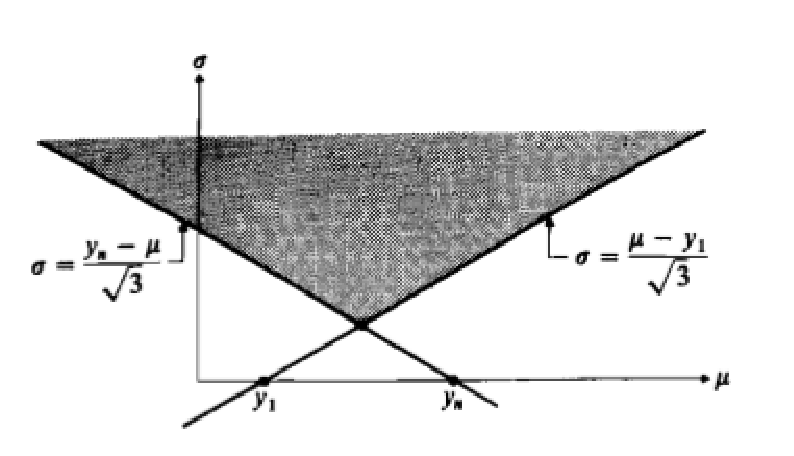
\includegraphics[scale = 0.5]{pictures/uniform_illustration.eps}
\caption{Konvergence k normálnímu rozdělení}
\label{uniform-illustration}
\end{figure}

Hodnota $(2 \sqrt{3} \sigma)^{-n}$ nabývá maxima pro minimální $\sigma$, které leží v průsečíku přímek $\mu - \sqrt{3} \sigma = y_1$ a $\mu + \sqrt{3} \sigma = y_n$. Proto odhady pro $\mu$ a $\sigma$ založené na funkci maximální věrohodnosti jsou
\begin{equation*}
\hat{\mu} = \frac{1}{2}(y_1 + y_n)
\end{equation*}
a
\begin{equation*}
\hat{\sigma} = \frac{1}{2 \sqrt{3}}(y_n - y_1)
\end{equation*}
\end{example}

\begin{theorem}[Invariance funkce odhadu metody maximální věrohodnosti]
Nechť $\hat{\Theta} = \zeta(X_1, ..., X_n)$ představuje funkci odhadu metody maximální věrohodnosti pro parametr $\theta$ pravděpodobnostní funkce $f(x, \theta)$. Předpokládejme, že $\theta$ je jednorozměrné. Dále uvažujme funkci $\tau(\cdot)$, k níž existuje jednorozměrná inverzní funkce. Pak platí, že funkce odhadu metody maximální věrohodnosti $\tau(\theta)$ je $\tau(\hat{\Theta})$.
\end{theorem}

\begin{example}
Uvažujme normální rozdělení s danou střední hodnotou $\mu_0$. Funkce odhadu parametru $\sigma^2$ je
\begin{equation*}
\hat{\Theta} = \frac{1}{n}\sum_{i = 1}^n (X_i - \mu_0)^2
\end{equation*}
Funkce odhadu parametru $\ln(\sigma^2)$ je pak
\begin{equation*}
\ln(\hat{\Theta}) = \ln\left(\frac{1}{n} \sum_{i = 1}^n (X_i - \mu_0)^2 \right)
\end{equation*}
\end{example}

Výše uvedenou větu lze dále zobecnit. Nechť $\theta = (\theta_1, ..., \theta_k)$ je $k$-rozměrný parametr a $\overline{\underline{\Theta}}$ představuje množinu všech možných $\theta$. Předmětem našeho zájmu je  odhad $\tau(\theta) = (\tau_1(\theta, ..., \tau_r(\theta))$, kde $1 \le r \le k$. Nechť $T$ představuje obor hodnot trasformace $\tau(\cdot) = (\tau_1(\cdot), ..., \tau_r(\cdot))$. To znamená, že $T$ je $r$-rozměrným prostorem. Definujme $M(\tau, x_1, ..., x_n) = \sup_{\{\theta: \tau(\theta) = \tau\}}L(\theta, x_1, ..., x_n)$\footnote{Označení $\sup$ v této knize má shodný význam jako v matematice. Čtenáři, kteří nejsou s tímto označením srozuměni, si namísto něj mohou dosadit pojmem $\max$.}. Tímto se dostáváme k následující větě.

\begin{theorem}
Uvažujme pravděpodobnostní funkci $f(\cdot, \theta_1, ..., \theta_k)$. Nechť $\hat{\Theta} = (\hat{\Theta}_1, ..., \hat{\Theta}_k)$, kde $\hat{\Theta}_j = \zeta_j(X_1, ..., X_n)$, je funkcí odhadu pro $\theta = (\theta_1, ..., \theta_k)$ dle metody maximální věrohodnosti. Nechť $\tau(\theta) = (\tau_1(\theta), ..., \tau_r(\theta))$ pro $1 \le r \le k$ představuje transformaci prostoru parametrů $\overline{\underline{\Theta}}$. Pak funkce odhadu pro $\tau(\theta) = (\tau_1(\theta), ..., \tau_r(\theta))$ dle metody maximální věrohodnosti má tvar $\tau(\hat{\Theta}) = (\tau_1(\hat{\Theta}), ..., \tau_r(\hat{\Theta}))$.
\end{theorem}

\begin{proof}
Nechť $\hat{\theta} = (\hat{\theta}_1, ..., \hat{\theta}_k)$ je odhadem pro $\theta = (\theta_1, ..., \theta_k)$. Stačí dokázat, že $M(\tau(\hat{\theta}), x_1, ..., x_n) \ge M(\tau, x_1, ..., x_n)$ pro libovolné $\tau \in T$. To vyplývá z nerovnosti $M(\tau, x_1, ..., x_n) = \sup_{\{\theta: \tau(\theta) = \tau \}}L(\theta, x_1, ..., x_n) \le \sup_{\theta \in \overline{\underline{\Theta}}} L(\theta, x_1, ..., x_n) = L(\hat{\theta}, x_1, ..., x_n) = \sup_{\{\theta: \tau(\theta) = \tau(\hat{\theta})\}}L(\theta, x_1, ..., x_n) = M(\tau(\hat{\theta}), x_1, ..., x_n)$.
\end{proof}

\begin{example}
Pro normální rozdělení platí $\theta = (\theta_1, \theta_2) = (\mu, \sigma^2)$. Uvažujme $\tau(\theta) = \mu + z_q\sigma$ kde $\phi(z_q) = q$ a $\tau(\theta)$ tak představuje $q$-tý kvantil. Dle výše uvedené věty je funkce odhadu pro $\tau(\theta)$ založená na metodě maximální věrohodnosti definována jako
\begin{equation*}
\overline{X} + z_q \sqrt{\frac{1}{n} \sum_{i = 1}^n (X_i - \overline{X})^2}
\end{equation*}
\end{example}

\subsection{Ostatní metody}

Existuje řada dalších metod bodového odhadu. Mezi tyto metody patří (a) metoda nejmenších čtverců, (b) Bayesova metoda, (c) chi-kvadrát metoda a (d) metoda nejmenší vzdálenosti. První dvě metody probereme později. V této kapitole se zaměříme na poslední dvě.

\subsubsection{Chi-kvadrát metoda}

Uvažujme náhodný výběr $X_1, ..., X_n$ z populace $f_X(x, \theta)$. Nechť $\mathscr{S}_1, ..., \mathscr{S}_k$ představuje rozpětí náhodné veličiny $X$ rozdělené na $k$ disjunktních intervalů. Pokusme se stanovit pravděpodobnost $p_j(\theta)$, s jakou pozorování připadne intervalu $\mathscr{S}_j$, kde $j = 1, ..., k$.

Jestliže je $f_X(x, \theta)$ pravděpodobnostní funkcí spojité náhodné veličiny, pak $p_j(\theta) = P[X ~ \textit{připadne intervalu} ~ \mathscr{S}_j] = \int_{\mathscr{S}_j}f_X(x, \theta) dx$. Z definice je zřejmé, že $\sum_{j = 1}^k p_j(\theta) = 1$. Nechť náhodná veličina $N_j$ představuje počet $X_i$ v náhodném výběru, která připadnou intervalu $\mathscr{S}_j$. Pak $\sum_{j = 1}^k N_j = n$, kde $n$ představuje velikost náhodného výběru. Definujme následující sumu
\begin{equation*}
\chi^2 = \sum_{j = 1}^k \frac{[n_j - n p_j(\theta)]^2}{n p_j(\theta)}
\end{equation*}
kde $n_j$ je hodnota náhodné veličiny $N_j$. Čitatel výše uvedené sumy je součtem kvadrátů rozdílu mezi skutečným a očekávaným počtem pozorování, která připadla intervalu $\mathscr{S}_j$. Odhad $\theta$ založený na chi-kvadrat metodě je takové $\hat{\theta}$, které minimalizuje $\chi^2$. Jedná se tedy o takové $\theta$ mezi všemi možnými $\theta$, pro které počet očekávaných pozorování ``nejbližší'' skutečnému počtu pozorování. Je zřejmé, že odhad $\hat{\theta}$ záleží na konkrétním výběru $\mathscr{S}_1, ..., \mathscr{S}_k$.

\begin{example}
Uvažujme náhodný výběr $X_1, ..., X_n$ z Bernoulliho rozdělení. Pravděpodobnostní funkce má tedy tvar $f_X(x, \theta) = \theta^x(1 - \theta)^{1 - x}$ pro $x = 0, 1$. Náhodná veličina $N_j$ představuje počet pozorování rovných $j = 0, 1$. Proto
\begin{gather*}
\chi^2 = \sum_{j = 0}^1 \frac{[n_j - n p_j(\theta)]^2}{n p_j(\theta)} = \frac{[n_0 - n(1 - \theta)]^2}{n(1 - \theta)} + \frac{(n_1 - n \theta)^2}{n \theta}\\
= \frac{[n - n_1 - n(1 - \theta)]^2}{n(1 - \theta)} + \frac{(n_1 - n \theta)^2}{n \theta} = \frac{(n_1 - n \theta)^2}{n} \frac{1}{\theta(1 - \theta)}
\end{gather*}
Minimum $\chi^2$ jako funkce $\theta$ nastavá v $\chi^2 = 0$ pro $\theta = \frac{n_1}{n}$. Proto $\hat{\theta} = \frac{n_1}{n}$.
\end{example}

Někdy je složité nalézt $\hat{\theta}$, které minimalizuje $\chi^2$. Proto bývá často $n p_j(\theta)$ ve jmenovateli nahrazeno $n_j$\footnote{Pokud $n_j = 0$, pak namísto $n_j$ použijeme 1.}. Pak hovoříme o tzv. modifikovaném $\chi^2$, které je definováno jako
\begin{equation*}
\chi^2_{mod} = \sum_{j = 1}^k \frac{[n_j - np_j(\theta)]^2}{n_j}
\end{equation*}
Tento modifikovaný odhad je opět založen na hodnotě $\hat{\theta}$, která minimalizuje $\chi^2_{mod}$.

\subsubsection{Metoda minimální vzdálenosti}

Nechť $X_1, ..., X_n$ představuje náhodný výběr z populace s kumulativní distribuční funkcí $F(X, \theta)$. Definujme funkci $d(F, G)$, která představuje vzdálenost mezi dvěma kumulativními distribučními funkcemi $F$ a $G$. Příkladem takovéto funkce může být $\sup_x|F(x) - G(x)|$, která představuje největší vertikální vzdálenost mezi funkcemi $F$ a $G$ a je ilustrována obrázkem (\ref{min-distance-function}).

\begin{figure}[htp]
\centering
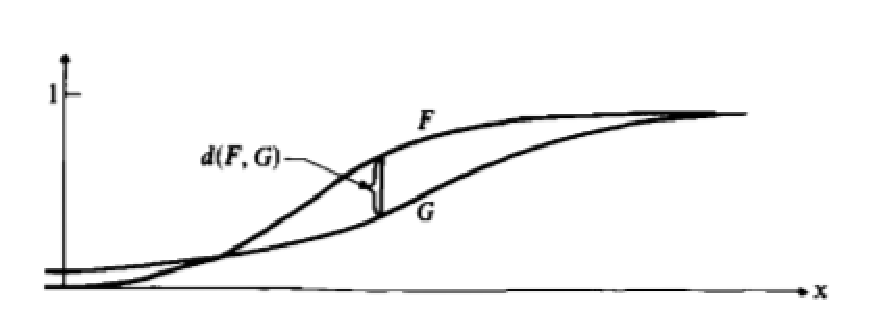
\includegraphics[scale = 0.5]{pictures/min_distance_function.eps}
\caption{Vzdálenost mezi dvěma kumulativními pravděpodobnostními funkcemi}
\label{min-distance-function}
\end{figure}

Odhad $\hat{\theta}$ parametru $\theta$ získaný pomocí metody minimální vzdálenosti je tedy představován takovou hodnotou, která minimalizuje $d(F(x, \theta), F_n(x))$, kde $F_n(x)$ je výběrovou kumulativní distribuční funkcí\footnote{Pouze připomeňme, že na základě teorie velkých čísel konverguje výběrová kumulativní distribuční funkce $F_n(x)$ ke kumulativní distribuční funkci $F(x)$ dané populace.}. Bohužel ne vždy je snadné určit hodnotu $\hat{\theta}$, která minimalizuje funkci vzdálenosti $d(F(x, \theta), F_n(x))$. Následující příklad je v tomto směru vyjímkou.

\begin{proof}
Nechť $X_1, ..., X_n$ představuje náhodný výběr z Bernoulliho rozdělení. Pak platí
\begin{equation*}
F(x, \theta) = (1 - \theta)I_{[0, 1)}(x) + I_{[1, \infty)}(x)
\end{equation*}
kde $0 \le \theta \le 1$. Dále nechť $n_j$ představuje počet pozorování rovných $j$, kde $j = 0, 1$. Pak zjevně platí
\begin{equation*}
F_n(x) = \frac{n_0}{n}I_{[0, 1)}(x) + I_{[1, \infty)}(x)
\end{equation*}
Jestliže použijeme funkci vzdálenosti $d(F,G) = \sup_x |F(x) - G(x)|$, pak tato funkce nabývá minima v bodě $1 - \theta = \frac{n_0}{n}$ neboli $\theta = \frac{n_1}{n} = \sum \frac{x_i}{n}$. Proto $\hat{\theta} = \overline{x}$.
\end{proof}.

\section{Vlastnosti funkcí odhadu}

V předchozím textu jsme ukázali několik metod bodového odhadu. Tímto vyvstává přirozená otázka, která z těchto metod je v dané situaci nejvhodnější.

\subsection{Blízkost funkce odhadu}

Uvažujme náhodný výběr $X_1, ..., X_n$ z populace $f(x, \theta)$. Funkce odhadu $\tau(\theta)$ je statistika, řekněme $\mathfrak{t}(X_1, ..., X_n)$, jejíž hodnota je použita jako odhad $\tau(\theta)$. V ideálním případě bychom chtěli, aby hodnota $\mathfrak{t}(X_1, ..., X_n)$ byla rovna hledané hodnotě $\tau(\theta)$. To však, s vyjímkou několika triviální případů, není možné.

\begin{example}
Uvažujme náhodný výběr z populace $f(x, \theta) = I_{(\theta - \frac{1}{2}, \theta + \frac{1}{2})}(x)$, kde $\theta$ je přirozené číslo. Je zřejmé, že $\theta$ je možné přesně odhadnout na základě jednoho pozorování $x_1$ a to tak, že $\mathfrak{t}(x_1)$ bude představovat hodnotu přirozeného čísla nejbližšího $x_1$.
\end{example}

Vzhledem k tomu, že $\mathfrak{t}(X_1, ..., X_n)$ není ve většině případů přesným odhadem $\tau(\theta)$, požadujeme, aby bylo alespoň ``blízkým'' odhadem. $T = \mathfrak{t}(X_1, ..., X_n)$ je statistika, která sleduje určité pravděpodobnostní rozdělení. Proto je logické požadovat, aby se hodnoty $t$ náhodné veličiny $T$ ``koncentrovaly'' poblíž $\tau(\theta)$.

\begin{definition}[Koncentrovaná a nejkoncentrovanější funkce odhadu]
Uvažujme dvě funkce odhadu $T = \mathfrak{t}(X_1, ..., X_n)$ a $T' = \mathfrak{t}'(X_1, ..., X_n)$ pro $\tau(\theta)$. Říkáme, že $T'$ je více koncentrované než $T$, jestliže
\begin{equation*}
P_{\theta}[\tau(\theta) - \lambda < T' \le \tau(\theta) + \lambda] \ge P_{\theta}[\tau(\theta) - \lambda < T \le \tau(\theta) + \lambda]
\end{equation*}
pro všechna $\lambda > 0$ a každé $\theta$ z $\overline{\underline{\Theta}}$. Funkci odhadu $T^* = \mathfrak{t}^*(X_1, ..., X_n)$ nazýváme nejkoncentrovanější funkcí odhadu, jestliže je více koncentrovaná než libovolná jiná funkce odhadu.
\end{definition}

Ve výše uvedené definici jsme použili značení $P_{\theta}[\cdot]$, abychom zdůraznili, že pravděpodobnost $P_{\theta}[\tau(\theta) - \lambda < T \le \tau(\theta) + \lambda]$ závisí na $\theta$ skrze pravděpodobnostní rozdělení $T$.

Vedle koncentrované a nejkoncentrovanější funkce odhadu existuje také obdobná Pitmanova definice blízké a nejbližší funkce odhadu.

\begin{definition}[Blízká a nejbližší funkce odhadu]
Uvažujme dvě funkce odhadu $T = \mathfrak{t}(X_1, ..., X_n)$ a $T' = \mathfrak{t}'(X_1, ..., X_n)$ pro $\tau(\theta)$. Říkáme, že $T'$ je více koncentrované než $T$, jestliže
\begin{equation*}
P_{\theta}[|T' - \tau(\theta)| < |T - \tau(\theta)|] \ge \frac{1}{2}
\end{equation*}
pro každé $\theta$ z $\overline{\underline{\Theta}}$. Funkci odhadu $T^* = \mathfrak{t}^*(X_1, ..., X_n)$ nazýváme nejbližší funkcí odhadu, jestliže je bližší než libovolná jiná funkce odhadu.
\end{definition}

Základní slabinou výše uvedených definic je skutečnost, že nejkoncentrovanější resp. nejbližší funkce odhadu existuje pouze ve vyjímečných případech. Důvodem je existence přílišného množství možných funkcí odhadu, než aby bylo možné některou z nich prohlásit za nejvhodnější. Navíc velmi často nelze ani tvrdit, že jedna funkce  odhadu je koncentrovanější resp. bližší než jiná, protože to se obvykle odvíjí od konkrétní hodnoty parametru $\theta$.

V předchozím textu jsme uvažovali fixní velikost náhodného výběru. Z pohledu ``blízkosti'' funkce odhadu je však také důležité, aby se přesnost odhadu zlepšovala s rostoucí velikostí náhodného výběru. V souvislosti s náhodným vzorkem dané velikosti hovoříme o vlastnostech funkce odhadu jako o vlastnostech malého výběru. O vlastnostech funkce odhadu, které jsou definované pro rostoucí velikost náhodného výběru, pak hovoříme jako o vlastnostech velkého výběru.

\subsection{Střední chyba čtverců}

\begin{definition}[MSE (mean-squared error) - střední chyba čtverců]
Nechť $T = \mathfrak{t}(X_1, ..., X_n)$ je funkcí odhadu pro $\tau(\theta)$. Pak $E_{\theta}[(T - \tau{\theta})^2]$ nazýváme MSE pro funkci odhadu $T = \mathfrak{t}(X_1, ..., X_n)$ a značíme ji jako $MSE_{\mathfrak{t}}(\theta)$.
\end{definition}

$\theta$ v případě $E_{\theta}[\cdot]$ indikuje pravděpodobnostní funkci, ze které pochází náhodný výběr. To znamená, že
\begin{gather*}
E_{\theta}[(T - \tau(\theta))^2] = E_{\theta}[(\mathfrak{t}(X_1, ..., X_n) - \tau(\theta))^2]\\
= \int \cdots \int (\mathfrak{t}(x_1, ..., x_n) - \tau(\theta))^2 f(x_1, \theta) \cdots f(x_n, \theta) dx_1 \cdots dx_n
\end{gather*}
kde $f(x, \theta)$ představuje pravděpodobnostní funkci populace.

Pokud porovnáváme funkce odhadu pomocí MSE, vybereme funkci s nejmenší MSE. Teoreticky je tak možné definovat funkci odhadu s nejmenší MSE, avšak stejně jako v předchozím případě, i zde je spíše vyjímkou, pokud takováto funkce existuje.

\begin{example}
Nechť $X_1, ..., X_n$ představuje náhodný výběr z $f(x, \theta)$, kde $\theta$ je reálné číslo. Předpokládejme, že předmětem zájmu je odhad parametru $\theta$, tj. $\tau(\theta) = \theta$.

Hledáme tedy funkci odhadu $T^* = \mathfrak{t}^*(X_1, ..., X_n)$ takovou, že $MSE_{\mathfrak{t}^*}(\theta) \le MSE_{\mathfrak{t}}(\theta)$ pro každé $\theta$ a libovolné $T = \mathfrak{t}(X_1, ..., X_n)$. Uvažujme rodinu funkcí odhadu $T_{\theta_0} = \mathfrak{t}_{\theta_0}(X_1, ..., X_n) \equiv \theta_0$ pro $\theta_0 \in \overline{\underline{\Theta}}$. Pro libovolné $\theta_0$ z $\overline{\underline{\Theta}}$ tedy funkce odhadu $T_{\theta_0}$ ``ignoruje'' pozorování a parametru $\theta$ přímo přiřadí hodnotu $\theta_0$. Všimněme si, že
\begin{equation*}
MSE_{\mathfrak{t}_{\theta_0}}(\theta) = E_{\theta}[(\mathfrak{t}(X_1, ..., X_n) - \theta)^2] = E_{\theta}[(\theta_0 - \theta)^2] = (\theta_0 - \theta)^2
\end{equation*}
Proto $MSE_{\mathfrak{t}_{\theta_0}}(\theta_0) = 0$. Má-li tedy existovat $T^* = \mathfrak{t}^*(X_1, ..., X_n)$, které splňuje $MSE_{\mathfrak{t}^*}(\theta) \le MSE_{\mathfrak{t}}(\theta)$ pro každé $\theta$ a funkci $\mathfrak{t}$, pak $MSE_{\mathfrak{t}^*} \equiv 0$. Aby funkce bodového odhadu $\mathfrak{t}^*$ měla MSE rovnu nule, musí parametr $\theta$ odhadnout vždy správně. To znamená, že musí být z náhodného výběru schopna vždy určit správnou hodnotu parametru $\theta$.
\end{example}

Jedním z důvodů, proč nejsme schopni nalézt funkci odhadu s nejmenší chybou čtverců je skutečnost, že počet potenciálních funkcí je příliš veliký. Tato množina pocentiálních funkcí také zahrnuje funkce, které jsou extrémně ``předpojaté'' ve prospěch určité konkrétní hodnoty parametru $\theta$\footnote{Jako ilustrace může posloužit funkce $\mathfrak{t}_{\theta_0}(X_1, ..., X_n)$ z předchozího příkladu, která byla ``předpojatá'' ve prospěch parametru $\theta_0$. Tato funkce totiž bez ohledu na reálný výsledek pozorování stanovila hodnotu parametru $\theta$ vždy rovnu $\theta_0$.}. Proto je vhodné množinu všech potencionálních funkcí odhadu omezit další podmínkou. Touto další podmínkou je podmínka nezkreslení.

\begin{definition}[Nezkreslená funkce odhadu]
O funkci odhadu $T = \mathfrak{t}(X_1, ..., X_n)$ říkáme, že je nezkreslená, tehdy a jen tehdy, jestliže
\begin{equation*}
E_{\theta}[T] = E_{\theta}[\mathfrak{t}(X_1, ..., X_n)] = \tau(\theta)
\end{equation*}
pro všechna $\theta = \overline{\underline{\Theta}}$.
\end{definition}

\begin{example}
Je tedy zřejmé, že funkce odhadu $\mathfrak{t}_{\theta_0}(X_1, ..., X_n)$ z předchozího příkladu není nezkreslenou funkcí odhadu parametru $\theta$, protože
\begin{equation*}
E_{\theta}[\mathfrak{t}_{\theta_0}(X_1, ..., X_n)] = E_{\theta}[\theta_0] = \theta_0 \neq \theta
\end{equation*}
\end{example}

\begin{corollary}
Jestliže je $T$ nezkreslenou funkcí odhadu pro $\tau(\theta)$, pak platí
\begin{equation*}
MSE_{\mathfrak{t}}(\theta) = D[T]
\end{equation*}
Toto tvrzení vyplývá ze vztahu
\begin{equation*}
MSE_{\mathfrak{t}}(\theta) = D[T] + (\tau(\theta) - E_{\theta}[T])^2
\end{equation*}
\end{corollary}

\begin{proof}
\begin{gather*}
MSE_{\mathfrak{t}}(\theta) = E_{\theta}[(T - \tau(\theta))^2] = E_{\theta}\left[\left((T - E_{\theta}[T]) - (\tau(\theta) - E_{\theta}[T])\right)^2 \right]\\
= E_{\theta}[(T - E_{\theta}[T])^2] - 2(\tau(\theta) - E_{\theta}[T])E_{\theta}[T - E_{\theta}[T]] + E_{\theta}[(\tau(\theta) - E_{\theta}[T])^2]\\
= D[T] + (\tau(\theta) - E_{\theta}[T])^2
\end{gather*}
\end{proof}

Člen $\tau(\theta) - E_{\theta}[T]$ nazýváme zkreslením funkce odhadu $T$. Tento člen může být kladný, záporný ale i nulový.

\begin{example}
Uvažujme náhodný výběr $X_1, ..., X_n$ z $f(x, \theta) = \phi_{\mu, \sigma^2}(x)$. Z příkladu (7.5) víme, že funkce odhadu dle metody maximální věrohodnosti pro parametr $\mu$ resp. $\sigma$ je $\overline{X}$ resp. $\frac{1}{n}\sum (X_i - \overline{X})^2$. Platí $E_{\theta}[\overline{X}] = \mu$, a proto je $\overline{X}$ nezkreslenou funkcí odhadu pro $\mu$. MSE funkce $\overline{X}$ je
\begin{equation*}
E_{\theta}[(\overline{X} - \mu)^2] = D[\overline{X}] = \frac{\sigma^2}{n}
\end{equation*}
Z předchozího textu také víme, že $E_{\theta}[S_n^2] = \sigma^2$, a proto
\begin{gather*}
E_{\theta}\left[\frac{1}{n} \sum_{i = 1}^n (X_i - \overline{X})^2 \right] = \frac{n - 1}{n}E_{\theta}\left[\frac{1}{n - 1} \sum_{i = 1}^n (X_i - \overline{X})^2 \right]\\
\frac{n - 1}{n}E[S_n^2] = \frac{n - 1}{n} \sigma^2
\end{gather*}
Funkce odhadu pro $\sigma$ tak je zkreslená. MSE pro $\frac{1}{n} \sum (X_i - \overline{X})^2$ lze s pomocí věty (6.2) vyjádřit jako
\begin{gather*}
E_{\theta}\left[\left(\frac{1}{n} \sum_{i = 1}^n (X_i - \overline{X})^2 - \sigma^2 \right)^2 \right] = D\left[\frac{1}{n} \sum_{i = 1}^n (X_i - \overline{X})^2 \right] + \left(\sigma^2 - E_{\theta}\left[\frac{1}{n} \sum_{i = 1}^n (X_i - \overline{X})^2 \right] \right)^2\\
= \frac{(n - 1)^2}{n^2}D[S_n^2] + \left(\sigma^2 - \frac{n - 1}{n} \sigma^2 \right)^2 = \frac{(n - 1)^2}{n^2}\frac{1}{n}\left(\mu_4 - \frac{n - 3}{n - 1}\sigma^4 \right) + \frac{\sigma^4}{n^2}
\end{gather*}
\end{example}

V následujícím textu bude MSE hlavním nástrojem pro posouzení funkce odhadu.

\subsection{Konzistentnost a BAN}

\begin{definition}[Konzistentnost ve smyslu MSE]
Nechť $T_1, ..., T_n$ představuje posloupnost funkcí odhadu pro $\tau(\theta)$, kde $T_n = \mathfrak{t}_n(X_1, ..., X_n)$ je definováno pro náhodný výběr velikosti $n$. Tuto posloupnost funkcí odhadu označujeme jako konzistentní ve smyslu MSE pouze tehdy a jen tehdy, jestliže
\begin{equation*}
\lim_{n \rightarrow \infty} E_{\theta}[(T_n - \tau(\theta))^2] = 0
\end{equation*}
pro všechna $\theta$ z $\overline{\underline{\Theta}}$.
\end{definition}

Konzistentnost ve smyslu MSE mimojiné znamená, že zkreslení a rozptyl $T_n$ se blíží nule s tím, jak se $n$ blíží nekonečnu, protože $E_{\theta}[(T_n - \tau(\theta))^2] = D[T_n] + (\tau(\theta) - E_{\theta}[T_n])^2$.

\begin{example}
Uvažujme náhodný výběr z pravděpodobnostního rozdělení se střední hodnotou $\mu$ a rozptylem $\sigma^2$. Nechť $\overline{X}_n = \frac{1}{n}\sum_{i = 1}^n X_i$ představuje posloupnost funkcí odhadu pro $\mu$ a $S_n^2 = \frac{1}{n - 1} \sum_{i = 1}^n (X_i - \overline{X}_n)$ pak posloupnost funkcí odhadu pro $\sigma^2$. Platí
\begin{equation*}
\lim_{n \rightarrow \infty} E[(\overline{X}_n - \mu)^2] = \lim_{n \rightarrow \infty} D[\overline{X}_n] = \lim_{n \rightarrow \infty} \frac{\sigma^2}{n} = 0
\end{equation*}
a proto je posloupnost $\{\overline{X}_n\}$ konzistení funkcí odhadu pro $\mu$. Dále platí
\begin{equation*}
\lim_{n \rightarrow \infty} E[(S_n^2 - \sigma^2)^2] = \lim_{n \rightarrow \infty} D[S_n^2] = \lim_{n \rightarrow \infty} \frac{1}{n} \left(\mu_4 - \frac{n - 3}{n - 1} \right) = 0
\end{equation*}
a proto také $\{S_n^2\}$ představuje konzistentní posloupnost funkcí odhadu pro $\sigma^2$. Všimněme si, že je-li $T_n = \frac{1}{n} \sum (X_i - \overline{X})^2$, pak je posloupnost $\{T_n\}$ konzistentní funkcí odhadu ve smyslu MSE nejen pro $\mu$ ale také pro $\sigma^2$.
\end{example}

Vedle výše uvedené definice existuje také ``slabší'' forma konzistence.

\begin{definition}[Slabší forma konzistence ve smyslu MSE]
Uvažujme posloupnost $T_1, ..., T_n$ funkcí odhadu pro $\tau(\theta)$, kde $T_n = \mathfrak{t}_n(X_1, ..., X_n)$. Posloupnost $\{T_n\}$ nazýváme ``slabě''  konzistentní ve smyslu MSE, jestliže je pro každé $\epsilon > 0$ a $\theta \in \overline{\underline{\Theta}}$ platí
\begin{equation*}
\lim_{n \rightarrow \infty} P_{\theta}[\tau(\theta) - \epsilon < T_n < \tau(\theta) + \epsilon] = 1
\end{equation*}
\end{definition}

\begin{proof}
S použitím Chebyshevovy nerovnosti lze dokázat
\begin{gather*}
P_{\theta}[\tau(\theta) - \epsilon < T_n < \tau(\theta) + \epsilon] = P[|T_n - \tau(\theta)| < \epsilon]\\
= P_{\theta}[(T_n - \tau(\theta))^2 < \epsilon^2] \ge 1 - \frac{E_{\theta}[(T_n - \tau(\theta))^2]}{\epsilon^2}
\end{gather*}
S tím, jak se $n$ blíží nekonečnu, se $E_{\theta}[(T_n - \tau(\theta))^2]$ blíží nule. Proto
\begin{equation*}
\lim_{n \rightarrow \infty} P_{\theta}[\tau(\theta) - \epsilon < T_n < \tau(\theta) + \epsilon] = 1
\end{equation*}
\end{proof}

Jestliže je funkce dhadu konzistentní, pak je také slabě konzistentní. Opačné tvrzení však neplatí.

\begin{definition}[BAN (best asymptotically normal) funkce odhadu]
Posloupnost funkcí bodového odhadu $T_1^*, ..., T_n^*$ pro $\tau(\theta)$ nazýváme BAN (best asymptotically normal), jestliže splňuje následující čtyři podmínky
\begin{enumerate}
\item Pravděpodobnostní rozdělení $\sqrt{n}[T_n^* - \tau(\theta)]$ se blíží normálnímu rozdělení s nulovou střední hodnotou a rozptylem $\sigma^{*2}(\theta)$ s tím, jak se $n$ blíží nekonečnu.
\item Pro každé $\epsilon > 0$ a každé $\theta \in \overline{\underline{\Theta}}$ platí
\begin{equation*}
\lim_{n \rightarrow \infty} P_{\theta}[|T^*_n - \tau(\theta)| > \epsilon] = 0
\end{equation*}
\item Nechť $\{T_n\}$ představuje libovolnou alternativní posloupnost slabě konzistentních funkcí odhadu s pravděpodobnostním rozdělením $\sqrt{n}[T_n - \tau(\theta)]$, které se blíží normálnímu rozdělení s nulovou střední hodnotou a rozptylem $\sigma^2(\theta)$.
\item $\sigma^2(\theta)$ není menší než $\sigma^{*2}(\theta)$ pro libovolný otevřený interval hodnot $\theta$.
\end{enumerate} 
\end{definition}

Namísto označení BAN se někdy používá CANE (consistent asymptotically normal efficient).

\begin{example}
Pro náhodné výběry z normálního rozdělení se střední hodnotou $\mu$ a rozptylem $\sigma^2$, je posloupnost $T^*_n = \frac{1}{n} \sum_{i = 1}^n X_i = \overline{X}_n$ je posloupností BAN pro $\mu$. Limitní pravděpodobnostní funkcí $\sqrt{n}(\overline{X}_n - \mu)$ je normální rozdělení s nulovou střední hodnotou a rozptylem $\sigma^2$. Žádná jiná funkce bodového odhadu nemůže mít menší rozptyl pro libovolný interval hodnot $\mu$. Nicméně existují i jiné BAN funkce bodového odhadu pro $\mu$, které mají shodné limitní normální rozdělení. Jako příklad uveďme
\begin{equation*}
T'_n = \frac{1}{n + 1} \sum_{i = 1}^n X_i
\end{equation*}
\end{example}

\subsection{Ztrátová a riziková funkce}

\begin{definition}[Ztrátová funkce]
Uvažujme odhad parametru $\tau(\theta)$. Nechť $t$ označuje hodnotu odhadu pro $\tau(\theta)$. Ztrátová funkce $\mathfrak{l}(t, \theta)$ je reálná funkce, která splňuje
\begin{enumerate}
\item $\mathfrak{l}(t, \theta) \ge 0$ pro všechny možné odhady $t$ a všechna $\theta \in \underline{\overline{\Theta}}$,
\item $\mathfrak{l}(t, \theta) = 0$ pro $t = \tau(\theta)$
\end{enumerate}
\end{definition}

Z logiky věci vyplývá, že ztrátová funkce by měla vracet  větší hodnoty pro větší odchylky $t$ od skutečné hodnoty $\tau(\theta)$ a naopak. Několik možných ztrátových funkcí je uvedeno v následujícím příkladu.

\begin{example}
~
\begin{enumerate}
\item $\mathit{l_1}(t, \theta) = (t - \tau(\theta))^2$
\item $\mathit{l_2}(t, \theta) = |t - \tau(\theta)|^2$
\item $\mathit{l_3}(t, \theta) = \begin{cases}A ~~~ \textit{pro} ~ |t - \tau{theta}| > \epsilon\\ 0 ~~~ \textit{pro} ~ |t - \tau{theta}| \le \epsilon \end{cases}$, kde $A > 0$
\item $\mathit{l_4}(t, \theta) = \rho(\theta)|t - \tau(\theta)|^r$ pro $\rho(\theta)$ a $r > 0$
\end{enumerate}
Funkce $\mathfrak{l}_1$ se nazývá ztrátová funkce chyby čtverců a funkce $\mathfrak{l}_2$ se nazývá ztrátová funkce absolutní chyby. Jak $\mathit{f}_1$ tak $\mathit{f}_2$ je rostoucí funkce chyby $t - \tau(\theta)$. Naproti tomu funkce $\mathfrak{l}_3$ nabývá pouze hodnot $A$ a 0 v závislosti na tom, zda-li se chyba $t- \tau(\theta)$ nachází v intervalu $\tau(\theta) \pm \epsilon$ či nikoliv. Konečně funkce $\mathfrak{l}_4$ je obecnou formou ztrátové funkce, která zahrnuje $\mathfrak{l}_1$ a $\mathfrak{l}_2$ jako specifické případy.
\end{example}

Při odhadu parametrů je naším cílem zvolit takovou funkci odhadu $T = \mathfrak{t}(X_1, ..., X_n)$, která bude minimalizovat ztrátovou funkci\footnote{Předpokládáme, že ztrátovou funkci známe. Volba vhodné ztrátové funkce však nemusí být tak jednoduchá, jak by se mohlo na první pohled zdát.}. Ztrátová funkce závisí na $t$, což je hodnota funkce bodového odhadu $T$. To znamená, že se hodnota ztrátové funkce odvíjí od konkrétního náhodného výběru $X_1 = x_1, ..., X_n = x_n$. Je zřejmé, že ztrátovou funkci nemůžeme minimalizovat pro každý možný náhodný výběr, avšak můžeme se ji pokusit minimalizovat v ``průměru''. Tímto se dostáváme k tzv. rizikové funkci.

\begin{definition}[Riziková funkce]
Pro danou ztrátovou funkci $\mathfrak{l}(t, \theta(t))$ a funkci bodového odhadu $T = \mathfrak{t}(X_1, ..., X_n)$ je riziková funkce definována jako
\begin{equation*}
\mathfrak{r}_t(\theta) = E_{\theta}[\mathfrak{t}(T, \theta)]
\end{equation*}
Riziková funkce tak představuje průměrnou hodnotu ztrátové funkce.
\end{definition}

Rizikovou funkci lze v zásadě vypočíst dvěma způsoby. Prvním z nich je pomocí sdružené pravděpodobnostní funkce náhodného výběru
\begin{gather*}
E_{\theta}[\mathfrak{l}(T, \theta)] = E_{\theta}[\mathfrak{l}(\mathfrak{t}(X_1, ..., X_n), \theta)]\\
= \int \cdots \int \mathfrak{l}(\mathfrak{t}(x_1, ..., x_n), \theta) \prod_{i = 1}^n f(x_i, \theta) d x_i
\end{gather*}
Druhý způsob se pak opírá o $T$ a její pravděpodobnostní funkci
\begin{gather*}
E_{\theta}[\mathfrak{l}(T, \theta)] = \int \mathfrak{l}(\cdot, \theta)f_T(t)dt
\end{gather*}

\begin{example}
Uvažujme ztrátové funkce z předchozího příkladu. Odpovídající rizikové funkce jsou
\begin{enumerate}
\item $E_{\theta}[(T - \tau(\theta))^2]$, což je již dříve uvedená MSE
\item $E_{\theta}[|T - \tau(\theta)|]$
\item $A \cdot P_{\theta}[|T - \tau(\theta)| > \epsilon]$
\item $\rho(\theta) E_{\theta}[|T - \tau(\theta)|^r]$
\end{enumerate}
\end{example}

\begin{definition}[Přijatelná funkce odhadu]
Uvažujme dvě funkce odhadu $T_1 = \mathit{t_1}(X_1, ..., X_n)$ a $T_2 = \mathit{t_2}(X_1, ..., X_n)$. Funkce odhadu $\mathfrak{t}_1$ je považována za nadřazenou funkci odhadu $\mathfrak{t}_2$ tehdy a jen tehdy, jestliže
\begin{equation*}
\mathit{R_{\mathfrak{t}_1}}(\theta) \ge \mathit{r_{\mathfrak{t}_2}}(\theta)
\end{equation*}
pro všechna $\theta \in \overline{\underline{\Theta}}$ a
\begin{equation*}
\mathit{R_{\mathfrak{t}_1}}(\theta) < \mathit{r_{\mathfrak{t}_2}}(\theta)
\end{equation*}
pro alespoň jedno $\theta \in \overline{\underline{\Theta}}$.
\end{definition}

Stejně jako v předchozích případech je také ztrátová funkce funkcí parametru $\theta$. Určení nejlepší funkce odhadu tak nemusí být jednoznačné. Částečným řešením tohoto problému je koncept tzv. minimaxu.

\begin{definition}[Minimax]
Funkci bodového odhadu $t^*$ nazýváme minimaxem tehdy a jen tehdy, jestliže
\begin{equation*}
\sup_{\theta} \mathfrak{r}(t^*)(\theta) \le \sup_{\theta} \mathfrak{r}_t(\theta)
\end{equation*}
pro každou alternativní funkci odhadu $\mathfrak{t}$.
\end{definition}

\section{Dostatečnost}

\subsection{Dostatečná statistika}

Uvažujme náhodný výběr $X_1, ..., X_n$ z populace $f(\cdot, \theta)$. Statistiku jsme definovali jako funkci náhodného výběru. Definičním oborem této funkce je množina všech hodnot, jichž může náhodný výběr $X_1, ..., X_n$ nabývat, a oborem hodnot je pak reálná osa. Na statistiku $T = \mathfrak{t}(X_1, ..., X_n)$ je také možno pohlížet jako na náhodnou veličinu. Funkce $\mathfrak{t}(\cdot, ..., \cdot)$ tedy transformuje $n$ náhodných veličin $X_1, ..., X_n$ do jedné náhodné veličiny. Předmětem našeho zájmu bude, zda-li při této transformaci dochází ke ztrátě informace či nikoliv.

Nechť $\mathfrak{X}$ označuje rozpětí hodnot, jichž může nabývat $(X_1, ..., X_n)$. Pomocí statistiky lze definovat segment prostoru $\mathfrak{X}$. Uvažujme statistiku $T = \mathfrak{t}(X_1, ..., X_n)$. Libovolná pozorování $(x_1, ..., x_n)$, pro která platí $t(x_1, ..., x_n) = t_0$, totiž představují segment prostoru $\mathfrak{X}$ definovaný hodnotou $T = t_0$.

\begin{example}
Uvažujme náhodný výběr $(X_1, X_2, X_3)$ z Bernoulliho rozdělení. Prostor $\mathfrak{X}$ se skládá z osmi bodů, a to $(0,0,0), (0,0,1), (0,1,0), (1,0,0), (0,1,1), (1,1,0), (1,0,1)$ a $(1,1,1)$. Definujme statistiku $T = X_1 + X_2 + X_3$. Tato statistika může nabývat čtyř hodnot, a proto rozděluje prostor $\mathfrak{X}$ na čtyři segmenty, a to  $\{(0,0,0)\}, \{(0,0,1), (0,1,0), (1,0,0) \}, \{(0,1,1), (1,1,0), (1,0,1)\}$ a $\{(1,1,1)\}$. Prostor $\mathfrak{X}$ by na shodné čtyři segmenty rozdělily také statistiky $T = 6(x_1 + x_2 + x_3)^2$ a $T = x_1^2 + x_2^2 + x_3^2$. Jestliže by tedy naším cílem bylo ``zredukovat'' prostor $\mathfrak{X}$, poskytly by nám všechny tyto tři statistiky stejnou službu.
\end{example}

\begin{definition}[Dostatečná statistika]
Uvažujme náhodný výběr $X_1, ..., X_n$ z populace $f(\cdot, \theta)$, kde $\theta$ může představovat jak skalár tak vektor. Předpokládejme, že funkční předpis $f(\cdot, \theta)$ je nám, s vyjímkou parametru $\theta$, znám. Statistika $S = \mathfrak{s}(X_1, ..., X_2)$ je dostatečná tehdy a jen tehdy, jestliže podmníněné pravděpodobnostní rozdělení $X_1, ..., X_n$ pro dané $S = s$ není funkcí $\theta$.
\end{definition}

Dostatečná statistika tedy zredukuje prostor $\mathfrak{X}$ takovým způsobem, že nedojde ke ztrátě informace o $\theta$. Ta je obsažena v náhodném výběru $X_1, ..., X_n$, což je důsledkem požadavku, aby podmíněné pravděpodobnostní rozdělení $X_1, ..., X_n$ nezáviselo na $\theta$. Nelze tedy očekávat, že získáme informaci o $\theta$ tím, že budeme provádět náhodný výběr z pravděpodobnostního rozdělení, které není funkcí $\theta$.

\begin{example}
Nechť $X_1, X_2, X_3$ představuje náhodný výběr z Bernoulliho rozdělení. Uvažujme dvě statistiky $S = \mathfrak{s}(X_1, X_2, X_3) = X_1 + X_2 + X_3$ a $T = \mathfrak{t}(X_1, X_2, X_3) = X_1X_2 + X_3$. Ukažme, že $S$ je na rozdíl od $T$ dostatečná statistika.
\begin{table}
\begin{center}
\begin{tabular}{| c | c | c | c | c |}
\hline
 & hodnoty $S$ & hodnoty $T$ & $f_{X_1, X_2, X_3|S}$ & $f_{X_1, X_2, X_3|T}$\\
\hline
$(0,0,0)$ & $0$ & $0$ & $1$ & $\frac{1 - p}{1 + p}$\\
\hline
$(0,0,1)$ & $1$ & $1$ & $\frac{1}{3}$ & $\frac{1 - p}{1 + 2p}$\\
\hline
$(0,1,0)$ & $1$ & $0$ & $\frac{1}{3}$ & $\frac{p}{1 + p}$\\
\hline
$(1,0,0)$ & $1$ & $0$ & $\frac{1}{3}$ & $\frac{p}{1 + p}$\\
\hline
$(0,1,1)$ & $2$ & $1$ & $\frac{1}{3}$ & $\frac{p}{1 + 2p}$\\
\hline
$(1,0,1)$ & $2$ & $1$ & $\frac{1}{3}$ & $\frac{p}{1 + 2p}$\\
\hline
$(1,1,0)$ & $2$ & $1$ & $\frac{1}{3}$ & $\frac{p}{1 + 2p}$\\
\hline
$(1,1,1)$ & $3$ & $2$ & $1$ & $1$\\
\hline
\end{tabular}
\caption{Dostatečná statistika}
\label{sufficient-statistics}
\end{center}
\end{table}

První sloupec tabulky (\ref{sufficient-statistics}) přestavuje prostor $\mathfrak{X}$. Podmíněné pravděpodobnosti lze vypočíst obvyklým způsobem. Jako příklad uveďme
\begin{gather*}
f_{X_1, X_2, X_3|S = 1}(0,1,0|1) = P[X_1 = 0, X_2 = 1, X_3 = 0 | S = 1]\\
= \frac{P[X_1 = 0, X_2 = 1, X_3 = 0, S = 1]}{P[S = 1]}\\
= \frac{(1 - p)p(1 - p)}{\binom{3}{1}p(1 - p)^2} = \frac{1}{3}
\end{gather*}
a
\begin{gather*}
f_{X_1, X_2, X_3|T = 0}(0, 1, 0 | 0) = \frac{P[X_1 = 0, X_2 = 1, X_3 = 0, T = 0]}{P[T = 0]}\\
= \frac{(1 - p)^2 p}{(1 - p)^3 + 2(1 - p)^2 p} = \frac{p}{1 - p + 2p} = \frac{p}{1 + p}
\end{gather*}
Podmíněná pravděpodobnostní funkce náhodného výběru pro danou hodnotu $S = s$ je nezávislá na parametru $p$, a proto je $S$ dostatečnou statistikou. Naproti tomu podmíněná pravděpodobnostní funkce náhodného výběru pro danou hodnotu $T = t$ je funkcí parametru $p$, a proto se o dostatečnou statistiku nejedná.

Všimněme si, že redukce prostoru $\mathfrak{X}$ pomocí statistiky $T$ je výraznější než pomocí statistiky $S$. Přirozenou otázkou je, zda-li existuje dostatečná statistika, která představuje větší redukci prostoru $\mathfrak{X}$ než $S$. Odpověď zní ``ne'' a lze ji dokázat zkoumáním množin všech segmentů prostoru $\mathfrak{X}$, které rozdělí tento prostor na tři a méně částí.
\end{example}

V případě náhodného výběru z pravděpodobnostní funkce spojité náhodné veličiny nemusí být význam pojmu ``podmíněné rozdělení $X_1, ..., X_n$ pro $S = s$'', který se objevuje v předchozí definici, na první pohled patrný, protože $P[S = s] = 0$. Existují dvě možné interpretace. První je založena na skutečnosti, že dostatečnost statistiky $S = \mathfrak{s}(X_1, ..., X_n)$ lze dokázat tím, že prokážeme nezávislost $P[X_1 \le x_1, ..., X_n \le x_n | S = s]$ na $\theta$, kde $P[X_1 \le x_1, ..., X_n \le x_n | S = s]$ je definováno ve smyslu $P[A|X = x] = \lim_{0 < h \rightarrow 0}P[A|x - h < X < x + h]$. Druhá interpretace je založena na transformaci jedna ku jedné z $X_1, ..., X_n$ na $S, Y_2, ..., Y_n$. Jestliže je pravděpodobnostní funkce $Y_2, ..., Y_n$ pro dané $S = s$ nezávislé na $\theta$, pak je $X_1, ..., X_n$ pro $S = s$ nezávislé na $\theta$, a $S$ tak představuje dostatečnou statistiku.

\begin{example}
Uvažujme náhodný výběr $X_1, X_2$ z populace $f(\cdot, \theta) = \phi_{\theta, 1}(\cdot)$ a statistiku $S = \mathfrak{s}(X_1, X_2) = X_1 + X_2$. Pokusme se dokázat, že $T$ je dostatečnou statistikou.

Začněme druhou z interpretací. Transformace z $(X_1, X_2)$ na $S, Y_2$, kde $S = X_1 + X_2$ a $Y_2 = X_2 - X_1$ je transformací jedna ku jedné, takže stačí dokázat, že $f_{Y_2|S}(y_2|s)$ je nezávislé na $\theta$. S využítím nezávislosti $X_1 + X_2$ a $X_2 - X_1$ lze dokázat, že
\begin{equation*}
f_{Y2|S}(y_2|s) = \frac{f_{Y_2, S}(y_2, s)}{f_S(s)} = \frac{f_{Y2}(y_2)f_S(s)}{f_S(s)} = f_{Y2}(y_2)
\end{equation*}
Zároveň však platí
\begin{equation*}
f_{Y_2}(y_2) = \frac{1}{\sqrt{2 \pi} \sqrt{2}}e^{-\frac{1}{2}\frac{y_2^2}{2}}
\end{equation*}
protože $Y_2 \sim N(0, 2)$. $f_{Y_2|S}(y_2|s)$ je tedy nezávislé na $\theta$ a $S$ je tak dostatečnou statistikou.

Důkaz pomocí druhé interpretace je poněkud složitější. V tomto případě musíme dokázat, že $P[X_1 \ge x_1, X_2 \ge x_2 | S = s]$ je nezávislé na $\theta$. Bez ztráty obecnosti můžeme předpokládat $x_1 \le x_2$ a rozlišovat tak tři základní případy
\begin{enumerate}
\item $s \le x_1$\\
\item $x_1 < s < x_2$\\
\item $x_2 < s$
\end{enumerate}
$P[X_1 \le x_1, X_2 \le x_2 | S = s]$ je pro třetí případ rovno nule a tudíž nezávislé na $\theta$. Důkaz dále ilustrujme pro první případ\footnote{Postup v druhém případě je analogický.}.
\begin{gather*}
P[X_1 \le x_1, X_2 \le x_2 | S = s] = \lim_{h \rightarrow 0}P[X_1 \le x_1, X_2 \le x_2 | s - h < S < s + h]\\
= \frac{\lim_{h \rightarrow 0} \frac{1}{2h} P[X_1 \le x_1, X_2 \le x_2, s - h < S < s + h]}{\lim_{h \rightarrow 0}\frac{1}{2h}P[s - h < S < s + h]}\\
= \frac{\lim_{h \rightarrow 0} \frac{1}{2h} P[X_1 \le x_1, X_2 \le x_2, s - h < S < s + h]}{f_S(s)}
\end{gather*}
Všimněme si, že
\begin{gather*}
\lim_{h \rightarrow 0} \frac{1}{2h} \int_{s + h - x_2}^{x_1} \int_{s - h - u}^{s + h - u} f_{X_1}(u)f_{X_2}(v)dv du\\
\le \lim_{h \rightarrow 0} \frac{1}{2h} P[X_1 \le x_1, X_2 \le x_2, s - h < X_1 + X_2 < s + h]\\
\le \lim_{h \rightarrow 0} \frac{1}{2h} \int_{s - h - x_2}^{x_1} \int_{s - h - u}^{s + h - u}f_{X_1}(u)f_{X_2}(v)dv du
\end{gather*}
a proto
\begin{gather*}
\lim_{h \rightarrow 0}\frac{1}{2h} P[X_1 \le x_1, X_2 \le x_2, s - h < X_1 + X_2 < s + h]\\
= \int_{s - x_2}^{x_1} f_{X_1}(u)f_{X_2}(s - u)du
\end{gather*}
Platí tedy
\begin{gather*}
P[X_1 \le x_1, X_2 \le x_2 | S = s] = \frac{\int_{s - x_2}^{x_1}f_{X_1}(u)f_{X_2}(s - u)du}{f_S(s)}\\
= \frac{\int_{s - x_2}^{x_1} \frac{1}{2 \pi} e^{-\frac{1}{2}[u^2 - 2u\theta + \theta^2 + (s - u)^2 - 2(s - u)\theta + \theta^2]}du}{\frac{1}{\sqrt{4 \pi}}e^{-\frac{1}{2}\left(\frac{s - 2\theta}{\sqrt{2}}\right)^2}}\\
= \frac{\frac{1}{\sqrt{2 \pi}} \int_{s - x_2}^{x_1} e^{-\frac{1}{2}[u^2 + (s - u)^2]}du}{\frac{1}{\sqrt{2}}e^{-\frac{1}{2}\frac{s^2}{2}}}
\end{gather*}
a podmíněná pravděpodobnost tak není funkcí $\theta$.
\end{example}

Výše uvedená definice dostatečné statistiky není v praxi příliš použitelná, protože vyžaduje odvození podmíněné pravděpodobobnostní funkce, což nemusí být vždy snadný úkol.

Následující definice je ekvivalentní s předcházející. Toto tvrzení však dokazovat nebudeme.

\begin{definition}[Dostatečná statistika]
Uvažujme náhodný výběr $X_1, ..., X_n$ z populace $f(\cdot, \theta)$. Statistika $S = s(X_1, ..., X_n)$ je dostatečnou statistikou tehdy a jen tehdy, jestliže podmíněná pravděpodobnost $T$ pro dané $S$ nezávisí na $\theta$ pro žádnou statistiku $T$.
\end{definition}

Tato definice je vhodná v situacích, kdy potřebujeme dokázat, že konkrétní statistika není dostatečná. Např. k dokázání toho, že $T' = \mathfrak{t}'(X_1, ..., X_n)$ není dostatečná, stačí nalézt jinou statistiku $T = \mathfrak{t}(X_1, ..., X_n)$, jejíž podmíněná pravděpodobnost pro dané $T'$ bude záviset na $\theta$.

V některých případech neexistuje dostatečná statistika. Vždy však existují sdruženě dostatečné statistiky.

\begin{definition}[Sdruženě dostatečné statistiky]
Uvažujme náhodný výběr $X_1, ..., X_n$ z populace $f(\cdot, \theta)$. Statistiky $S_1, ..., S_r$ jsou sdruženě dostatečné tehdy a jen tehdy, jestliže podmíněná pravděpodobnost $X_1, ..., X_n$ pro $S_1 = s_1, ..., S_r = s_r$ nezávisí na $\theta$.
\end{definition}

Náhodný výběr $X_1, ..., X_n$ je sám o sobě vždy sdruženě dostatečný, protože jeho podmíněná pravděpodobnost nezávisí na $\theta$\footnote{Podmíněná pravděpodobnost tohoto náhodného výběru je totiž podmíněna sama sebou. Je totiž zřejmé, že $P[X_1 = x_1, ..., X_n = x_n | X_1 = x_1, ..., X_n = x_n] = 1$.}. Také pořadové statistiky $Y_1, ..., Y_n$ jsou sdruženě dostatečné. Pro dané $Y_1 = y_1, ..., Y_n = y_n$ totiž $X_1, ..., X_n$ musí být některou z permutací $y_1, ..., y_n$. Vzhledem k tomu,že těchto permutací je $n!$ a vzhledem k tomu, že se jedná o náhodný výběr, je pravděpodobnost realizace jednotlivých permutací shodná, a proto $P[X_1 = x_1, ..., X_n = x_n | Y_1 = y_1, ..., Y_n = y_n] = \frac{1}{n!}$, což je nezávislé na $\theta$.

Připomeňme, že nejdůležitější úlohou dostatečné statistiky je rozdělit prostor $\mathfrak{X}$ a množinu segmentů. Hodnoty, kterých přitom nabývá, pravidla nejsou předmětem zájmu. Platnost následující věty je pak patrná.

\begin{definition}
Jestliže statistiky $S_1 = \mathit{s_1}(X_1, ..., X_n), ..., S_r = \mathit{s_r}(X_1, ..., X_n)$ jsou sdruženě dostatečné, pak je libovolný soubor jejich funkcí jedna ku jedné popř. transformací jedna ku jedné je taktéž sdruženě dostatečný.
\end{definition}

\begin{example}
Jsou-li $\sum X_i$ a $\sum X_i^2$ sdruženě dostatečné, pak $\overline{X}$ a $\sum (X_i - \overline{X})^2 = \sum X_i^2 - n\overline{X}$ jsou taktéž sdruženě dostatečné. Naproti tomu $\overline{X}^2$ a $\sum(X_i - \overline{X})^2$ nemusí být sdruženě dostatečné, protože se nejedná o funkce jedna ku jedné pro $\sum X_i$ a $\sum X_i^2$.
\end{example}

\subsection{Kritérium rozkladu}

\begin{theorem}[Kritérium rozkladu pro dostatečnou statistiku]
Uvažujme náhodný výběr $X_1, ..., X_n$ z populace $f(\cdot, \theta)$. Statistika $S = \mathfrak{s}(X_1, ..., X_n)$ je dostatečná právě tehdy a jen tehdy, jestliže sdruženou pravděpodobnost $X_1, ..., X_n$, která má tvar $\prod_{i = 1}^n f(x_i, \theta)$, lze vyjádřit pomocí rozkladu
\begin{gather*}
f_{X_1, ..., X_n}(x_1, ..., x_n, \theta) = g(\mathfrak{s}(x_1,..., x_n), \theta)h(x_1, ..., x_n)\\
= g(s, \theta)h(x_1, ..., x_n)
\end{gather*}
kde $h(x_1, ..., x_n)$ je nezáporná funkce, která neobsahuje $\theta$ a $g(\mathfrak{s}(x_1, ..., x_n), \theta)$ je nezáporná funkce, která závisí na $x_1, ..., x_n$ pouze skrze funkci $\mathfrak{s}(\cdot, ..., \cdot)$. 
\end{theorem}

\begin{theorem}[Kritérium rozkladu pro sdruženě dostatečné statistiky]
Uvažujme náhodný výběr $X_1, ..., X_n$ z populace $f(\cdot, \theta)$. Statistiky $S_1 = \mathit{s_1}(X_1, ..., X_n), ..., S_r = \mathit{s_r}(X_1, ..., X_n)$ jsou sdruženě dostatečné právě tehdy a jen tehdy, jestliže sdruženou pravděpodobnost $X_1, ..., X_n$ lze vyjádřit pomocí rozkladu
\begin{gather*}
f_{X_1, ..., X_n}(x_1, ..., x_n, \theta) = g(\mathfrak{s}_1(x_1,..., x_n), ..., \mathfrak{s}_r(x_1, ..., x_n), \theta)h(x_1, ..., x_n)\\
= g(s_1, ..., s_r, \theta)h(x_1, ..., x_n)
\end{gather*}
kde $h(x_1, ..., x_n)$ je nezáporná funkce, která neobsahuje $\theta$ a $g(\mathfrak{s}_1, ..., \mathfrak{s}_r, \theta)$ je nezáporná funkce, která závisí na $x_1, ..., x_n$ pouze skrze funkce $\mathfrak{s}_1, ..., \mathfrak{s}_r$.
\end{theorem}

Výše uvedené dvě věty získají intuitivní základ, pokud si uvědomíme následující. Jestliže lze provést rozklad sdružené pravděpodobnostní funkce, pak je funkce maximální věrohodnosti proporcionální funkci $g(s, \theta)$, která závisí na porozorováních $x_1, ..., x_n$ pouze skrze funkci $\mathfrak{s}$. Funkce $h(x_1, ..., x_n)$ vystupuje v rámci funkce maximální věrohodnosti jako konstanta. Funkce maximální věrohodnosti je tak pouze funkcí $\theta$. To znamená, že informace ohledně $\theta$, které funkce maximální věrohodnosti ``obsahuje'', je obsažena ve statistice $s(\cdot, ..., \cdot)$. 

\begin{example}
Uvažujme náhodný výběr $X_1, ..., X_n$ z Bernoulliho rozdělení s parametrem $\theta$, tj.
\begin{equation*}
f(x, \theta) = \theta^x (1 - \theta)^{1-x}I_{(0,1)}(x) ~~~ 0 \le \theta \le 1
\end{equation*}
Pak platí
\begin{equation*}
\prod_{i = 1}^n f(x_i, \theta) = \prod_{i = 1}^n \theta^{x_i}(1 - \theta)^{1 - x_i}I_{(0,1)}(x_i) = \theta^{\sum x_i}(1 - \theta)^{n - \sum x_i}\prod_{i = 1}^n I_{(0, 1)}(x_i)
\end{equation*}
Jestliže dosadíme $g(\mathfrak{s}(x_1, ..., x_n)) = \theta^{\sum x_i}(1 - \theta)^{n - \sum x_i}$, $h(x_1, ..., x_n) = \prod_{i = 1}^n I_{(0,1)}(x_i)$ a $\mathfrak{s}(x_1, ..., x_n) = \sum x_i$, pak je sdružená pravděpodobnostní funkce $X_1, ..., X_2$ dána větou (7.3), což znamená, že statistika $S = \mathfrak{s}(X_1, ..., X_n) = \sum X_i$ je dostatečná.
\end{example}

\begin{example}
Uvažujme náhodný výběr z populace $\phi_{\theta, 1}(\cdot)$. Sdružená pravděpodobnostní funkce je rovna
\begin{gather*}
f_{X_1, ..., X_n}(x_1, ..., x_n, \theta) = \prod_{i = 1}^n \phi_{\theta,1}(x_i) = \prod_{i = 1}^n \frac{1}{\sqrt{2 \pi}}e^{-\frac{1}{2}(x_i - \theta)^2}\\
= \frac{1}{(2 \pi)^{\frac{n}{2}}}e^{-\frac{1}{2}\sum_{i = 1}^n(x_i - \theta)^2} = \frac{1}{(2 \pi)^{\frac{n}{2}}}e^{-\frac{1}{2}(\sum x_i^2 - 2 \theta \sum x_i + n \theta^2)}\\
= \frac{1}{(2 \pi)^{\frac{n}{2}}}e^{\theta \sum x_i - \frac{n}{2}\theta^2}e^{-\frac{1}{2}\sum x_i^2}
\end{gather*}
Jestliže dosadíme $h(x_1, ..., x_n) = \frac{1}{(2 \pi)^{n/2}}e^{-1/2 \sum x_i^2}$, $g(\mathfrak{s}(x_1, ..., x_n), \theta) = e^{\theta \sum x_i - (n/2)\theta}$ a $\mathfrak{s}(x_1, ..., x_n) = \sum x_i$, pak je sdružená pravděpodobnostní funkce $X_1, ..., X_n$ dána větou (7.4), což znamená, že statistika $S = \mathfrak{s}(X_1, ..., X_n) = \sum X_i$ je dostatečná.

Připomeňme, že statistika $\overline{X}_n$ je taktéž dostatečná, protože libovolná funkce jedna ku jedné dostatečné statistiky je také dostatečná statistika. 
\end{example}

\begin{example}
Uvažujme náhodný výběr $X_1, ..., X_n$ z populace $\phi_{\mu, \sigma^2}$. V tomto případě je $\theta$ vektor dvou parametrů, tj. $\theta = (\mu, sigma)$. Sdružená pravděpodobnost $X_1, ..., X_n$ je dána
\begin{gather*}
f_{X_1, ..., X_n}(x_1, ..., x_n, \theta) = \prod_{i = 1}^n \phi_{\mu, \sigma^2}(x_i) = \prod_{i = 1}^n \frac{1}{\sqrt{2 \pi} \sigma} e^{-\frac{1}{2}\left(\frac{x_i - \mu}{\sigma}\right)^2}\\
= \frac{1}{(2 \pi)^{\frac{n}{2}}}\sigma^{-n}e^{-\frac{1}{2}\sum \left(\frac{x_i - \mu}{\sigma}\right)^2}\\
= \frac{1}{(2 \pi)^{\frac{n}{2}}}\sigma^{-n}e^{-\frac{1}{2 \sigma^2}\left(\sum x_i^2 - 2 \mu \sum x_i + n \mu^2 \right)}
\end{gather*}
Sdružená pravděpodobnostní funkce tak závisí na pozorováních $x_1, ..., x_n$ pouze skrze statistiky $\mathfrak{s}_1(x_1, ..., x_n) = \sum x_i$ a $\textit{s}_2(x_1, ..., x_n) = \sum x_i^2$ a je dána větou (7.5), kde $h(x_1, ..., x_n) = 1$. Statistiky $\sum X_i$ a $\sum X_i^2$ jsou tak sdruženě dostatečné.

Vzhledem k tomu, že $\overline{X}_n$ a $S_n^2 = \frac{1}{n - 1}\sum (X_i - \overline{X}_n)^2$ jsou funkcemi jedna ku jedné sdruženě dostatečných statistik $\sum X_i$ a $\sum X_i^2$, jsou také $\overline{X}_n$ a $S_n^2$ sdruženě dostatečné.
\end{example}

\begin{example}
Uvažujme náhodný výběr $X_1, ..., X_n$ z uniformního rozdělení nad intervalem $[\theta_1, \theta_2]$, tj. $\theta = (\theta_1, \theta_2)$. Sdružená pravděpodobnostní funkce $X_1, ..., X_n$ je dána
\begin{gather*}
f_{X_1, ..., X_n}(x_1, ..., x_n, \theta) = \prod_{i = 1}^n \frac{1}{\theta_2 - \theta_1}I_{[\theta_1, \theta_2]}(x_i)\\
= \frac{1}{(\theta_2 - \theta_1)^n} \prod_{i = 1}^n I_{[\theta_1, \theta_2]}(x_i) = \frac{1}{(\theta_2 - \theta_1)^n}I_{[\theta_1, y_n]}(y_1)I_{[y_1, \theta_2]}(y_n)
\end{gather*}
kde $y_1 = \min(x_1, ..., x_n)$ a $y_n = \max(x_1, ..., x_n)$. Sdružená pravděpodobnost tak závisí na $x_1, ..., x_n$ pouze skrze $y_1$ a $y_n$, a její rozklad je dán větou (7.5), kde $h(x_1, ..., x_n) = 1$. Statistiky $Y_1$ a $Y_n$ jsou sdruženě dostatečné.

Všimněme si, že pro $\theta_1 = \theta^*$ a $\theta_2 = \theta^* + 1$, jsou $Y_1$ a $Y_n$ stále sdruženě dostatečné. Jestliže však $\theta_1 = 0$ a $\theta_2 = \theta^*$, pak se náš rozklad změní na
\begin{equation*}
f_{X_1, ..., X_n}(x_1, ..., x_n, \theta^*) = \frac{1}{\theta^{*n}} \prod_{i = 1}^n I_{[0, \theta^*]}(x_i) = \frac{1}{\theta^{*n}}I_{[0, \theta]}(y_n)I_{[0, y_n]}(y_1)
\end{equation*}
Jestliže dosadíme $g(\mathfrak{s}(x_1, ..., x_n), \theta) = \frac{1}{\theta^{*n}}I_{[0, \theta]}(y_n)$ a $h(x_1, ..., x_n) = I_{[0, y_n]}(y_1)$ a $h(x_1, ..., x_n) = I_{[0, y_n]}(y_1)$, je zřejmé, že statistika $Y_n$ je dostatečná sama o sobě.
\end{example}

\begin{theorem}
Funkce (popř. soubor funkcí) maximální věrohodnosti závisí na náhodném výběru skrze libovolný soubor sdruženě dostatečných statistik.
\end{theorem}

\begin{proof}
Jestliže $S_1 = \mathfrak{s}_1(X_1, ..., X_n), ..., S_k = \mathfrak{s}_k(X_1, ..., X_n)$ jsou sdruženě dostatečné statistiky, pak lze funkci maximální věrohodnosti zapsat ve tvaru
\begin{gather*}
L(\theta, x_1, ..., x_2) = \prod_{i = 1}^n f(x_i, \theta)\\
= g(\mathfrak{s}_1(x_1, ..., x_n), ..., \mathfrak{s}_k(x_1, ..., x_n), \theta)h(x_1, ..., x_n)
\end{gather*}
Funkce maximální věrohodnosti tedy má maximum ve stejném bodě jako funkce $g(s_1, ..., s_k)$. Maximum funkce $g(\cdot, ..., \cdot)$ může být ovlivněno hodnotami $s_1, ..., s_k$, které jsou však dány pozorováními $x_1, ..., x_n$.
\end{proof}

\subsection{Minimální dostatečná statistika}

Hlavní myšlenkou dostatečné statistiky je redukce dat bez ztráty informace o parametrech výběrové populace. Z předchozího textu je zřejmé, že existuje více než jedna dostatečná statistika popř. více než jeden soubor sdruženě dostatečných statistik. V případě normálního rozdělení s neznámou střední hodnotou a rozptylem mohou roli dostatečných sdružených statistik plnit (a) samotný náhodný výběr $X_1, ..., X_n$, (b) jeho pořadová statistika $Y_1, ..., Y_n$ a (c) statistiky $\overline{X}_n$ a $S_n^2$. Logicky preferujeme sdruženě dostatečné statistiky $\overline{X}_n$ a $S_n^2$, protože míra, s kterou redukují původní data $X_1, ..., X_n$, je větší než u prvních dvou příkladů. Přirozenou otázkou je, zda-li existuje nějaký jiný soubor dostatečných statistik, které redukují data více než $\overline{X}_n$ a $S_n^2$. Odpověď zní nikoliv, avšak nemáme (a ve zbytku knihy a ani nebudeme mít) aparát, s jehož pomocí bysme toto tvrzení dokázali. Nicméně tyto úvahy nás přivedly k pojmu minimální dostatečná statistika.

Jak jsme již dříve zmínili, každá statistika odpovídá určitému regionu v prostoru $\mathfrak{X}$. Zjednodušeně řečeno platí, že míra redukce dat dané statistiky je dána počtem podmnožin v tomto regionu. Minimální dostatečná statistika je pak taková statistika, které má v daném regionu menší počet podmnožin než jakákoliv jiná alternativní statistika. Analogické tvrzení platí pro soubor statistik.

\begin{theorem}[Minimální dostatečná statistika]
Soubor sdruženě dostatečných statistik je minimálně dostatečný tehdy a jen tehdy, jestliže se jedná o funkci všech ostatních souborů dostatečných statistik.
\end{theorem}

Výše uvedená definice nám bohužel není příliš nápomocná při hledání sdruženě minimálních dostatečných statistik. Ty je možné nalézt vhodným rozkladem jejich sdružené pravděpodobností funkce. Konkrétní postup však přesahuje rámec této knihy.

\subsection{Rodina exponenciálních rozdělení}

\begin{definition}[Rodina jednoparametrických exponenciálních rozdělení]
Je-li $\theta$ skalárem, pak pravděpodobnostní funkce $f(\cdot, \theta)$ spojité náhodné veličiny, kterou lze pro $-\infty < x < \infty$, všechna $\theta \in \overline{\underline{\Theta}}$ a vhodně zvolené funkce $a(\cdot), b(\cdot), c(\cdot), d(\cdot)$ vyjádřit ve tvaru
\begin{equation*}
f(x, \theta) = a(\theta)b(x)e^{c(\theta) d(x)}
\end{equation*}
patří do rodiny exponenciálních rozdělení.
\end{definition}

\begin{example}
Je-li $f(x, \theta) = \theta e^{- \theta x}I_{(0, \theta)}(x)$, pak $f(x, \theta)$ náleží do rodiny exponenciálních funkcí, protože $a(\theta) = \theta, b(x) = I_{(0, \infty)}(x), c(\theta) = - \theta$ a $d(x) = x$.
\end{example}

\begin{example}
Je-li $f(x, \theta) = f(x, \lambda)$ Poissonovo rozdělení, pak
\begin{equation*}
f(x, \lambda) = \frac{e^{-\lambda}\lambda^x}{x!}I_{\{0, 1, ... \}}(x) = e^{-\lambda}\left(\frac{1}{x!}I_{\{0, 1, ...\}}(x)\right)e^{x~ln(\lambda)}
\end{equation*}
Poissonovo rozdělení tak náleží do rodiny exponenciální rozdělení, protože $a(\lambda) = e^{-\lambda}, b(x) = \frac{1}{x!}I_{\{0, 1, ...\}}(x), c(\lambda) = \ln(\lambda)$ a $d(x) = x$.
\end{example}

Jestliže $f(x, \theta) = a(\theta)b(x)e^{c(\theta)d(x)}$, pak
\begin{equation*}
\prod_{i = 1}^n f(x, \theta) = a^n(\theta)\left[\prod_{i = 1}^n b(x_i) \right]e^{c(\theta) \sum_{i = 1}^n d(x_i)}
\end{equation*}
a proto je $\sum d(X_i)$ dostatečnou statistikou. To znamená, že náleží-li pravděpodobnostní rozdělení do rodiny jednoparametrických exponenciálních rozdělení, pak vždy existuje dostatečná statistika. Lze dokázat, že takto získaná dostatečná statistika je zároveň minimální.

\begin{definition}[Rodina víceparametrických exponenciálních rozdělení]
Pravděpodobnostní rozdělení $f(\cdot, \theta_1, ..., \theta_k)$ spojitých náhodných veličin, které lze pro vhodně zvolené funkce $a(\cdot, ..., \cdot), b(\cdot), c_j(\cdot, ..., \cdot)$ a $d_j(\cdot)$ vyjádřit ve tvaru
\begin{equation*}
f(x, \theta, ..., \theta_k) = a(\theta_1, ..., \theta_k)b(x)e^{\sum_{j = 1}^k c_j(\theta_1, ..., \theta_k)d_j(x)}
\end{equation*}
náleží do rodiny exponenciálních rozdělení.
\end{definition}
 
\begin{example}
Je-li $f(x, \theta_1, \theta_2) = \phi_{\mu, \sigma^2}(x)$, kde $(\theta_1, \theta_2) = (\mu, \sigma)$, pak $f(x; \theta_1, \theta_2)$ náleží do rodiny exponenciálních rozdělení.
\begin{gather*}
f(x;\theta_1, \theta_2) = \frac{1}{\sqrt{2 \pi} \sigma} e^{-\frac{1}{2}\left(\frac{x - \mu}{\sigma}\right)^2}\\
= \frac{1}{\sqrt{2 \pi} \sigma} e^{-\frac{1}{2}\frac{\mu^2}{\sigma^2}}e^{-\frac{1}{2 \sigma^2}x^2 + \frac{\mu}{\sigma^2}x}
\end{gather*}
protože $a(\mu, \sigma) = \frac{1}{\sqrt{2 \pi}\sigma}e^{-1/2\mu^2/\sigma^2}, b(x) = 1, c_1(\mu, \sigma) = -1/2\sigma^2, c_2(\mu, \sigma) = \mu^2/\sigma^2, d_1(x) = x^2$ a $d_2(x) = x$.
\end{example}

\begin{example}
Jestliže
\begin{equation*}
f(x; \theta_1, \theta_2) = \frac{1}{B(\theta_1, \theta_2)}x^{\theta_1 - 1}(1 - x)^{\theta_2 - 1}I_{(0, 1)}(x)
\end{equation*}
pak
\begin{equation*}
f(x; \theta_1, \theta_2) = \frac{1}{B(\theta_1, \theta_2)}I_{(0, 1)}(x)e^{(\theta_1 - 1)\ln(x) + (\theta_2 - 1)\ln(1 - x)}
\end{equation*}
kde $a(\theta_1, \theta_2) = \frac{1}{B(\theta_1, \theta_2)}, b(x) = I_{(0, 1)}(x), c_1(\theta) = \theta_1 - 1, c_2(\theta_1, \theta_2) = \theta_1 - 1, c_2(\theta_1, \theta_2) = \theta_2 - 1, d_1(x) \ln(x)$ a $d_2(x) = \ln(1 - x)$.
\end{example}

Uvažujme náhodný výběr z populace
\begin{equation*}
f(x; \theta_1, ..., \theta_k) = a(\theta_1, ..., \theta_k)b(x)e^{\sum_{j = 1}^k c_j(\theta_1, ..., \theta_k)d_j(x)}
\end{equation*}
pak platí
\begin{equation*}
\prod_{i = 1}^n f(x_i; \theta_1, ..., \theta_k) = a^n(\theta_1, ..., \theta_k)\left[\prod_{i = 1}^n b(x_i)\right]e^{\sum_{j = 1}^k c_j(\theta_1, ..., \theta_k) \sum_{i = 1}^n d_j(x_i)}
\end{equation*}
a proto $\sum_{i = 1}^n d_1(X_i), ..., \sum_{i = 1}^n d_k(X_i)$ představuje soubor sdruženě dostatečných statistik. Zároveň se jedná o minimální sdruženě dostatečné statistiky.

\begin{example}
Pro výše uvedený příklad náhodného výběru z beta rozdělení jsou statistiky $\sum_{i = 1}^n \ln (X_i)$ a $\sum_{i = 1}^n \ln(1 - X_i)$ minimální sdruženě dostatečné statistiky.
\end{example}

\section{Nezkreslený odhad}
 
Připomeňme, že dle tvrzení (7.1) platí
\begin{equation*}
E_{\theta}[(T - \tau(\theta))^2] = D_{\theta}[T] + (\tau(\theta) - E_{\theta}[T])^2
\end{equation*}
Jestliže je tedy $T$ nezkreslenou funkcí odhadu pro $\tau(\theta)$, pak $E_{\theta}[T] = \tau(\theta)$, a proto $E_{\theta}[(T - \tau(\theta))^2] = D_{\theta}[T]$.

\begin{definition}[UMVUE (uniformly minimum variance unbiased estimator)]
Uvažujme náhodný výběr $X_1, ..., X_n$ z populace $f(\cdot, \theta)$. Funkce odhadu $T^* = \mathfrak{t}^*(X_1, ..., X_n)$ pro $\tau(\theta)$ je UMVUE (uniformly minimum-variance unbiased estimator) pro $\tau(\theta)$ tehdy a jen tehdy, jestliže
\begin{enumerate}
\item $E_{\theta}[T^*] = \tau(\theta)$, tj. $T^*$ je nezkreslenou funkcí odhadu
\item $D_{\theta}[T^*] \le D_{\theta}[T]$ pro libovolnou alternativní funkci odhadu $T = \mathfrak{t}(X_1, ..., X_n)$, která splňuje $E_{\theta}[T] = \tau(\theta)$.
\end{enumerate}
\end{definition}

\subsection{Dolní mez rozptylu}

Uvažujme náhodný výběr $X_1, ..., X_n$ z populace $f(\cdot, \theta)$, kde $\theta \in \overline{\underline{\Theta}}$. Předpokládejme, že $\overline{\underline{\Theta}}$ je podmnožinou reálné osy a že $T = \mathfrak{t}(X_1, ..., X_n)$ je nezkreslená funkce odhadu pro $\tau(\theta)$. V následujícím textu je $f(\cdot, \theta)$ pravděpodobnostní funkcí spojité náhodné veličiny; v případě nespojité náhodné veličiny je postup analogický. Předpokládejme, že jsou splněny tzv. podmínky regularity.
\begin{enumerate}
\item Pro všechna $x$ a $\theta$ existuje
\begin{equation*}
\frac{\partial}{\partial \theta} \ln(f(x,\theta))
\end{equation*}
\item
\begin{gather*}
\frac{\partial}{\partial \theta} \int \cdots \int \prod_{i = 1}f(x_i, \theta)dx_1 \cdots dx_n\\
= \int \cdots \int \frac{\partial}{\partial \theta} \prod_{i = 1}^n f(x_i, \theta)dx_1 \cdots dx_n
\end{gather*}
\item
\begin{equation*}
\frac{\partial}{\partial \theta} \int \cdots \int \mathfrak{t}(x_1, ..., x_n) \prod_{i = 1}^n f(x_i, \theta)dx_1 \cdots dx_n = \int \cdots \int \mathfrak{t}(x_1, ..., x_n) \frac{\partial}{\partial \theta} \prod_{i = 1}^n f(x_i, \theta)dx_1 \cdots dx_n
\end{equation*}
\item Pro všechna $\theta \in \overline{\underline{\Theta}}$ platí
\begin{gather*}
0 < E_{\theta}\left[\left(\frac{\partial}{\partial \theta} \ln(f(X, \theta))\right)^2\right] < \infty
\end{gather*}
\end{enumerate}

\begin{theorem}[Cramér-Raova nerovnost]
Při splnění výše uvedených čtyř podmínek regularity platí
\begin{equation*}
D_{\theta}[T] \ge \frac{[\tau'(\theta)]^2}{n E_{\theta}\left[\left(\frac{\partial}{\partial \theta} \ln(f(X, \theta))\right)^2\right]}
\end{equation*}
kde $T = \mathfrak{t}(X_1, ..., X_n)$ je nezkreslenou funkcí odhadu pro $\tau(\theta)$. Rovnost ve výše uvedeném vztahu nastane tehdy a jen tehdy, jestliže existuje funkce $K(\theta, n)$ taková, že
\begin{equation*}
K(\theta, n)[\mathfrak{t}(x_1, ..., x_n) - \tau(\theta)] = \sum_{i = 1}^n \frac{\partial}{\partial \theta}\ln(f(x_i, \theta))
\end{equation*}
Nerovnost uvedená v této větě je tzv. Cramér-Raovou nerovností a její pravá strana se nazývá Cramér-Raovou dolní hranicí rozptylu nezkreslené funkce odhadu pro $\tau(\theta)$.
\end{theorem}

\begin{proof}
\begin{gather*}
\tau'(\theta) = \frac{\partial}{\partial \theta} \tau(\theta) = \frac{\partial}{\partial \theta} \int \cdots \int \mathfrak{t}(x_1, ..., x_2) \prod_{i = 1}^n f(x_i, \theta) dx_1 \cdots dx_n\\
= \int \cdots \int \mathfrak{t}{x_1, ..., x_n}\frac{\partial}{\partial \theta}\left[\prod_{i = 1}^n f(x_i, \theta) \right] dx_1 \cdots dx_n - \tau(\theta)\frac{\partial}{\partial \theta} \int \cdots \int \prod_{i = 1}^n [f(x_i, \theta)dx_i]\\
= \int \cdots \int \mathfrak{t}{x_1, ..., x_n}\frac{\partial}{\partial \theta}\left[\prod_{i = 1}^n f(x_i, \theta) \right] dx_1 \cdots dx_n - \tau(\theta) \int \cdots \int \frac{\partial}{\partial \theta}\left[\prod_{i = 1}^n f(x_i, \theta)\right]dx_1 \cdots dx_n\\
= \int \cdots \int[\mathfrak{t}(x_1, ..., x_n) - \tau(\theta)]\frac{\partial}{\partial \theta}\left[\prod_{i = 1}^n f(x_i, \theta)\right]dx_1 \cdots dx_n\\
= \int \cdots \int[\mathfrak{t}(x_1, ..., x_n) - \tau(\theta)]\left[\frac{\partial}{\partial \theta}\ln \left(\prod_{i = 1}^n f(x_i, \theta)\right)\right] \times \prod_{i = 1}^n f(x_i, \theta) dx_1 \cdots dx_n\\
= E_{\theta}\left[[\mathfrak{t}(X_1, ..., X_n) - \tau(\theta)]\left[\frac{\partial}{\partial \theta} \ln \left(\prod_{i = 1}^n f(x_i, \theta)\right)\right]\right]
\end{gather*}
S využitím Cauchy-Schwarzovy nerovnosti platí
\begin{equation*}
[\tau'(\theta)]^2 \le E_{\theta}[(\mathfrak{t}(X_1, ..., X_n) - \tau(\theta))^2]E_{\theta}\left[\left(\frac{\partial}{\partial \theta}\ln \left(\prod_{i = 1}^n f(X_i, \theta) \right)\right)^2\right]
\end{equation*}
neboli
\begin{equation*}
D_{\theta}[T] \ge \frac{[\tau'(\theta)]^2}{E_{\theta}\left[\left(\frac{\partial}{\partial \theta}\ln \left(\prod_{i = 1}^n f(x_i, \theta) \right) \right)^2 \right]}
\end{equation*}
Zároveň však, s využitím nezávislosti $X_i$ a $X_j$ a vztahu
\begin{gather*}
E_{\theta} \left[\frac{\partial}{\partial \theta} \ln \left(f(X, \theta)\right)\right] = \int\left(\frac{\partial}{\partial \theta} \ln \left(f(x, \theta)\right)\right)f(x, \theta)dx\\
= \int \frac{\partial}{\partial \theta} f(x, \theta)dx = \frac{\partial}{\partial \theta}\int f(x, \theta)dx = \frac{\partial}{\partial \theta}(1) = 0
\end{gather*}
lze dokázat
\begin{gather*}
E_{\theta}\left[\left(\frac{\partial}{\partial \theta}\ln \left(\prod_{i = 1}^n f(X_i, \theta)\right) \right)^2 \right] = E_{\theta}\left[\left(\sum_{i = 1}^n \frac{\partial}{\partial \theta} \ln \left(f(X_i, \theta)\right) \right)^2\right]\\
= \sum_i \sum_j E_{\theta}\left[\left(\frac{\partial}{\partial \theta} \ln \left(f(X_i, \theta) \right)\right)\left(\frac{\partial}{\partial \theta} \ln \left(f(X_i, \theta) \right)\right)\right] = n E_{\theta}\left[\left(\frac{\partial}{\partial \theta} \ln \left(f(X, \theta)\right)\right)^2\right]
\end{gather*}

Cauchy-Schwarzova nerovnost se stane rovností tehdy a jen tehdy, jestliže je jedna funkce násobkem druhé. To v našem případě znamená, že $\frac{\partial}{\partial \theta} \ln \left(\prod_{i = 1}^n f(x_i, \theta) \right)$ je násobkem $\mathfrak{t}(x_1, ..., x_n) - \tau(\theta)$. Jinými slovy musí existovat taková funkce $K(\theta, n)$, aby platilo
\begin{equation*}
\frac{\partial}{\partial \theta} \ln \left(\prod_{i = 1}^n f(x_i, \theta) \right) = K(\theta, n)[\mathfrak{t}(x_1, ..., x_n) - \tau(\theta)]
\end{equation*}
\end{proof}

V případě nespojitých náhodných veličin, je třeba modifikovat podmínky regularity, věta o Cramér-Raově nerovnosti však zůstává beze změny.

Z Cramér-Raovy nerovnosti vyplývá, že pokud má daná funkce odhadu rozptyl, který odpovídá dolní hranici rozptylu dle této nerovnosti, pak se jedná jedná o UMVUE. Jestliže existuje $T^* = \mathfrak{t}^*(X_1, ..., X_n)$ taková, že
\begin{equation*}
\sum_{i = 1}^n \frac{\partial}{\partial \theta} \ln \left(f(x_i, \theta)\right) = K(\theta, n)[\mathfrak{t}^*(x_1, ..., x_n) - \tau^*(\theta)]
\end{equation*}
pro vhodně zvolenou funkci $K(\theta, n)$ a $\tau^*(\theta)$, pak je $T^*$ je UMVUE pro $\tau^*(\theta)$.

\begin{example}
Uvažujme náhodný výběr $X_1, ..., X_n$ z populace $f(x, \theta) = \theta e^{-\theta x}I_{(0, \infty)}(x)$. Lze dokázat, že pro uvažovanou pravděpodobnostní funkci jsou splněny podmínky regularity.

Nechť $\tau(\theta) = \theta$. Protože $\tau'(\theta) = 1$ platí
\begin{equation*}
D_{\theta}[T] \ge \frac{1}{nE_{\theta}\left[\left(\frac{\partial}{\partial \theta} \ln \left(f(X, \theta)\right)\right)^2\right]}
\end{equation*}
Všimněme si, že $\frac{\partial}{\partial \theta} \ln \left(f(x, \theta) \right) = \frac{\partial}{\partial \theta}(\ln(\theta) - \theta x) = \frac{1}{\theta} - x$, a proto
\begin{equation*}
E_{\theta}[\left(\frac{\partial}{\partial \theta} \ln \left(f(X, \theta)\right)\right)^2] = E_{\theta}\left[\left(\frac{1}{\theta} - X\right)^2\right] = D[X] = \frac{1}{\theta^2}
\end{equation*}
Cramér-Raova dolní hranice rozptylu nezkreslené funkce odhadu pro $\theta$ je tak
\begin{equation*}
D_{\theta}[T] \ge \frac{1}{n(1 / \theta^2)} = \frac{\theta^2}{n}
\end{equation*}

Nechť $\tau(\theta) = 1/\theta$. Cramér-Raova dolní hranice rozptylu nezkreslené funkce odhadu je dána
\begin{equation*}
D_{\theta}[T] \ge \frac{[\tau'(\theta)]^2}{n(1/\theta^2)} = \frac{1}{n \theta^2}
\end{equation*}
Levá strana druhé rovnice věty (7.7) je
\begin{equation*}
\sum_{i = 1}^n \frac{\partial}{\partial \theta}\ln \left(f(x_i, \theta) \right) = \sum_{i = 1}^n \frac{\partial}{\partial \theta}\left(\ln(\theta) - \theta x_i \right) = \sum_{i = 1}^n \left(\frac{1}{\theta} - x_i \right) = -n \left(\overline{x}_n - \frac{1}{\theta}\right)
\end{equation*}
Vzhledem k tomu, že $K(\theta, n) = -n$, je $\overline{X}$ UMVUE pro $1/\theta$, protože se její rozptyl shoduje s Cramér-Raovou dolní hranicí rozptylu.
\end{example}

\begin{example}
Uvažujme náhodný výběr $X_1, ..., X_n$ z populace $f(x, \theta) = f(x, \lambda) = e^{-\lambda}\lambda^x / x!$ pro $x = 0, 1, 2, ...$. Platí
\begin{gather*}
\frac{\partial}{\partial \lambda} \ln \left(f(x, \lambda)\right) = \frac{\partial}{\partial \lambda} \ln \left(\frac{e^{-\lambda}\lambda^x}{x!}\right)\\
= \frac{\partial}{\partial \lambda}(-\lambda + x \ln(\lambda) - \ln(x!)) = -1 + \frac{x}{\lambda} 
\end{gather*}
Proto
\begin{gather*}
E\left[\left(\frac{\partial}{\partial \lambda} \ln\left(f(X, \lambda)\right)\right)^2\right] = E\left[\left(\frac{X}{\lambda} - 1\right)^2\right] = \frac{1}{\lambda^2}E[(X - \lambda)^2]\\
= \frac{1}{\lambda^2}D[X] = \frac{1}{\lambda^2}{\lambda} = \frac{1}{\lambda}
\end{gather*}
Jmenovatel Cramér-Raovy nerovnosti je tedy $n/\lambda$. Jestliže $\tau(\lambda) = e^{-\lambda} = P[X = 0]$, pak je Craméer-Raova dolní hranice rozptylu pro nezkreslenou funkci odhadu dána
\begin{equation*}
D[T] \ge \frac{\lambda e^{-2 \lambda}}{n}
\end{equation*}
Statistika $T = \frac{1}{n}\sum_{i = 1}^n I_{\{0\}}(X_i)$ je nezkresleným odhadem $\tau(\lambda) = e^{-\lambda}$, protože 
\begin{equation*}
E[T] = \frac{1}{n}\sum_{i = 1}^n E[I_{\{0\}}(X_i)] = \frac{1}{n}\sum_{i = 1}^n e^{-\lambda} = e^{-\lambda}
\end{equation*}
Jestliže $X_i = 0$, pak $I_{\{0\}}(X_i) = 1$; v ostatních případech je $I_{\{0\}}(X_i)$ rovno nule. Proto $E[I_{\{0\}}(X_i)] = 1 \cdot P[X_i = 0] + 0 \cdot P[X_i \neq 0] = e^{-\lambda}$. $T$ tak představuje relativní podíl pozorování rovných nule. Pro její rozptyl platí
\begin{equation*}
D[T] = \frac{1}{n}e^{-\lambda}(1 - e^{-\lambda})
\end{equation*}
Odpovídající Cramér-Raova dolní mez prozptylu je $\frac{1}{n}\lambda e^{-2 \lambda}$. Všimněme si, že skutečně platí
\begin{equation*}
\frac{1}{n}e^{-\lambda}(1 - e^{-\lambda}) \ge \frac{1}{n}\lambda e^{-2 \lambda}
\end{equation*}
Dále platí
\begin{equation*}
\sum_{i = 1}^n \frac{\partial}{\partial \lambda} \ln \left(f(x, \lambda)\right) = \sum_{i = 1}^n \left(-1 + \frac{x_i}{\lambda}\right) = \frac{n}{\lambda}(\overline{x} - \lambda)
\end{equation*}
a proto je $\overline{X}$ UMVUE pro $\lambda$.
\end{example}

Za určitých předpokladů zahrnujících existenci druhých derivací a zaměnitelnosti pořadí pro vybrané integrace a derivace platí
\begin{equation*}
E_{\theta}\left[\left(\frac{\partial}{\partial \theta} ln \left(f(X, \theta)\right)\right)^2\right] = - E_{\theta}\left[\frac{\partial^2}{\partial^2}\ln\left(f(X, \theta)\right)\right]
\end{equation*}
Tento vztah může být užitečný v případě, kde je složitější vypočíst střední hodnotu na levé straně rovnosti než střední hodnotu na pravé straně rovnosti.

\begin{theorem}
Jestliže je odhad $\hat{\theta} = \hat{\zeta}(x_1, ..., x_n)$ parametru $\theta$ získaný metodou maximální věrohodnoti dán řešením rovnice
\begin{equation*}
\frac{\partial}{\partial \theta}\ln\left(L(\theta, x_1, ..., x_n)\right) \equiv \frac{\partial}{\partial \theta}\ln \left(\prod_{i = 1}^n f(x_i, \theta) \right) = 0
\end{equation*}
a jestliže $T^* = \mathfrak{t}^*(X_1, ..., X_n)$ je nezkreslenou funkcí odhadu pro $\tau^*(\theta)$ a její rozptyl se shoduje s Cramér-Raovou dolní mezí rozptylu, pak $\mathfrak{t}^*(x_1, ..., x_n) = \tau^*(\hat{\zeta}(x_1, ..., x_n))$.
\end{theorem}

\begin{proof}
S využitím druhé rovnice věty (7.7) lze dokázat
\begin{equation*}
0 = \frac{\partial}{\partial \theta}\ln \left(\prod_{i = 1}^n f(x_i, \theta)\right)\Big|_{\theta = \hat{\theta}} = K(\theta, n)[\mathfrak{t}^*(x_1, ..., x_n) - \tau^*(\theta)]\Big|_{\theta = \hat{\theta}}
\end{equation*}
\end{proof}

Výše uvedená věta nám tedy říká, že při splnění zde uvedených podmínek je funkce odhadu získaná metodou maximální věrohodnosti UMVUE.

Následující tvrzení ponecháme bez důkazu. Uvažujme pravděpodobnostní funkci $f(\cdot, \theta)$. Nechť je $T^* = \mathfrak{t}^*(X_1, ..., X_n)$ nezkreslenou funkcí odhadu pro $\tau^*(\theta)$, jejíž rozptyl se shoduje s Cramér-Raovou dolní mezí rozptylu. Pak je $f(\cdot, \theta)$ členem rodiny exponenciálních rozdělení. Toto tvrzení platí také naopak. Je-li $f(\cdot, \theta)$ členem rodiny exponenciálních rozdělení, pak existuje nezkreslená funkce odhadu $T^*$ pro $\tau^*(\theta)$, jejíž rozptyl se shoduje s Cramér-Raovou dolní mezí rozptylu. Bohužel nám toto tvrzení také nepřímo říká, že statistiku, jejíž rozptyl se shoduje s Cramér-Raovou dolní mezí rozptylu, jsme schopni nalézt pouze v případě, že pravděpodobnostní funkce populace náleží do rodiny exponenciálních rozdělení. Cramér-Raova dolní mez rozptylu je tak užitečná pro nalezení UMVUE pouze, jestliže náhodný výběr pochází z rodiny exponenciálních rozdělení s jedním parametrem. V takovém případě navíc existuje pouze jedna jediná funkce (kromě lineárních funkcí této funkce) tohoto parametru, pro kterou existuje nezkreslená funkce odhadu a jejíž rozptyl se shoduje s Cramér-Raovou dolní mezí rozptylu. Proto je třeba při identifikaci UMVUE aplikovat jiný postup.

\subsection{Dostatečnost a kompletnost}

\begin{theorem}[Rao-Blackwellova]
Uvažujme náhodný výběr $X_1, ..., X_n$ z populace $f(\cdot, \theta)$. Nechť $S_1 = {s_1}(X_1, ..., X_n), ..., S_k = \mathfrak{s}_k(X_1, ..., X_n)$ jsou sdruženě dostatečné statistiky a $T = \mathfrak{t}(X_1, ..., X_n)$ představuje nezkreslenou funkci odhadu pro $\tau(\theta)$. Definujme $T' = E[T|S_1, ..., S_k]$. Pak
\begin{enumerate}
\item $T'$ je statistikou a jedná se o funkci sdruženě dostatečných statistik $S_1, ..., S_k$. Proto $T' = \mathit{t'}(S_1, ..., S_k)$.
\item $E_{\theta}[T'] = \tau(\theta)$, což znamená, že $T'$ je nezkreslenou funkcí odhadu pro $\tau(\theta)$.
\item $D_{\theta}[T'] \le D_{\theta}[T]$ pro každé $\theta$ a  $D_{\theta}[T'] < D_{\theta}[T]$ pro alespoň některá $\theta$, pokud není $T$ rovno $T'$ s pravděpodobností 1.
\end{enumerate}
\end{theorem}

\begin{proof}
~
\begin{enumerate}
\item $S_1, ..., S_k$ jsou sdruženě dostatečné statistiky. Pro daná $S_1, ..., S_k$ je tak statistika $T$ nezávislá na $\theta$. Proto je $T' = E[T|S_1, ..., S_k]$ taktéž nezávislé na $\theta$ a $T'$ lze tedy chápat jako stastistiku, která je funkcí $S_1, ..., S_k$.
\item S pomocí věty (4.11) lze dokázat
\begin{equation*}
E_{\theta}[T'] = E_{\theta}[E[T|S_1, ..., S_k]] = E[T] = \tau(\theta)
\end{equation*}
\item Rozptyl statistiky $T$ lze vyjádřit jako
\begin{gather*}
D_{\theta}[T] = E_{\theta}[(T - E_{\theta}[T'])^2] = E_{\theta}[(T - T' + T' - E_{\theta}[T'])^2]\\
= E_{\theta}[(T - T')^2] + 2 E_{\theta}[(T - T')(T' - E_{\theta}[T'])] + D_{\theta}[T']
\end{gather*}
Zároveň však platí
\begin{equation*}
E_{\theta}[(T - T')(T' - E_{\theta}[T'])] = E_{\theta}[E[(T - T')(T' - E_{\theta}[T'])|S_1, ..., S_k]]
\end{equation*}
a
\begin{gather*}
E[(T - T')(T' - E_{\theta}[T'])|S_1 = s_1, ..., S_k = s_k]\\
= \left(\mathfrak{t}'(s_1, ..., s_k) - E_{\theta}[T']\right)E[(T - T')|S_1 = s_1, ..., S_k = s_k]\\
= \left(\mathfrak{t}'(s_1, ..., s_k) - E_{\theta}[T']\right)\left(E[T|S_1 = s_1, ..., S_k = s_k] - E[T'|S_1 = s_1, ..., S_k = s_k]\right)\\
= \left(\mathfrak{t}'(s_1, ..., s_k) - E_{\theta}[T']\right)\left(\mathfrak{t}'(s_1, ..., s_k) - \mathfrak{t}'(s_1, ..., s_k)\right) = 0
\end{gather*}
a proto
\begin{equation*}
D_{\theta}[T] = E_{\theta}[(T - T')^2] + D_{\theta}[T'] \ge D_{\theta}[T']
\end{equation*}
Všimněme si, že $D_{\theta}[T] > D_{\theta}[T']$ pokud se $T$ nerovná $T'$ s pravděpodobností 1.
\end{enumerate}
\end{proof}

\begin{example}
Uvažujme náhodný výběr $X_1, ..., X_n$ z Bernoulliho rozdělení $f(x, \theta) = \theta^x(1 - \theta)^{1 - \theta}$ pro $x = 0, 1$. $X_1$ je nezkreslená funkce odhadu pro $\tau(\theta) = \theta$. Použijme $X_1$ jako $T = \mathfrak{t}(X_1, ..., X_n)$. Vzhledem k tomu, že $\sum X_i$ je dostatečná statistika, použijme $S = \sum X_i$ jako dostatečnou statistiku. Dle výše uvedené věty je $T' = E[T|S] = E[X_1|\sum X_i]$ nezkreslenou funkcí odhadu pro $\theta$ s rozptylem ne větším než má statistika $T = X_1$. Pokusme se vypočíst $E[T|S]$.

V prvním kroku je třeba vypočíst podmíněnou pravděpodobnost $X_1$ pro $\sum X_i = s$. Připomeňme, že $X_1$ může nabývat pouze hodnot 0 a 1.
\begin{gather*}
P[X_1 = 0 | \sum_{i = 0}^n X_1 = s] = \frac{P\left[X_1 = 0, \sum_{i = 1}^n X_i = s\right]}{P\left[\sum_{i = 1}^n X_i = s\right]} = \frac{P\left[X_i = 0, \sum_{i = 2}^n X_i = s\right]}{P\left[\sum_{i = 1}^n X_i = s\right]}\\
= \frac{P[X_1 = 0] \cdot P\left[\sum_{i = 2}^n X_i = s \right]}{P\left[\sum_{i = 1}^n X_i = s\right]} = \frac{(1 -\theta)\binom{n - 1}{s}\theta^s(1 - \theta)^{n - 1 - s}}{\binom{n}{s}\theta^s(1 - \theta)^{n - s}} = \frac{n - s}{n}
\end{gather*}
\begin{gather*}
P\left[X_1 = 1 | \sum_{i = 1}^n X_i = s \right] = \frac{P\left[X_1 = 1, \sum_{i = 1}^n X_i = s \right]}{P\left[\sum_{i = 1}^n X_i = s \right]} = \frac{P\left[X_1 = 1, \sum_{i = 2}^n X_i = s - 1\right]}{P\left[\sum_{i = 1}^n X_i = s \right]}\\
= \frac{P[X_1 = 1]\cdot P\left[\sum_{i = 2}^n X_i = s - 1 \right]}{P\left[\sum_{i = 1}^n X_i = s \right]} = \frac{\theta \binom{n - 1}{s - 1}\theta^{s - 1}(1 - \theta)^{n - 1 - s + 1}}{\binom{n}{s}\theta^s(1 - \theta)^{n - s}} = \frac{s}{n}
\end{gather*}
Podmíněná pravděpodobnost $X_1$ pro dané $\sum X_i = s$ je nezávislá na $\theta$. Definujme
\begin{equation*}
T' = \frac{\sum_{i = 1}^n X_i}{n}
\end{equation*}
Rozptyl $X_1$ je $\theta(1 - \theta)$ a rozptyl $T'$ je $\frac{\theta(1 - \theta)}{n}$. Pro $n > 2$ je tak rozptyl $T'$ menší než rozptyl $T = X_1$.
\end{example}

Jestliže je funkce odhadu $T$ již pouze funkcí $S_1, ..., S_k$, pak bude odvozená statistika $T'$ totožná s $T$. Ačkoliv $S_1, ..., S_k$ představuje libovolný soubor sdruženě dostatečných statistik, přirozeně preferujeme minimální sdruženě dostatečné statistiky.

\begin{definition}[Kompletní rodina rozdělení]
Uvažujme náhodný výběr $X_1, ..., X_n$ z populace $f(\cdot, \theta)$ a statistiku $T = \mathfrak{t}(X_1, ..., X_n)$. Rodina pravděpodobnostních rozdělení statistiky $T$ je kompletní tehdy a jen tehdy, jestliže $E_{\theta}[\mathit{z}(T)] \equiv 0$ pro všechna $\theta \in \overline{\underline{\Theta}}$ implikuje $P_{\theta}[\mathit{z}z(T) = 0] \equiv 1$ pro všechna $\theta \in \overline{\underline{\Theta}}$, pro která je $\mathit{z}(T)$ statistikou. O statistice $T$ říkáme, že je kompletní tehdy a jen tehdy, jestliže je její rodina pravděpodobnostních rozdělení kompletní.
\end{definition}

\begin{example}
Uvažujme náhodný výběr $X_1, ..., X_n$ z Bernoulliho rozdělení.

Statistika $T = X_1 - X_2$ není kompletní, protože $E_{\theta}[X_1 - X_2] = 0$, ale $X_1 - X_2$ není rovno nule s pravděpodobností 1.

Uvažujme statistiku $T = \sum_{i = 1}^n X_i$. Nechť $\mathit{z}(T)$ je libovolná statistika, která je funkcí $T$ a pro kterou platí $E_{\theta}[z(T)] \equiv 0$ pro všechna $0 \le \theta \le 1$. Abychom dokázali, že je $T$ kompletní, musíme dokázat, že $\mathit{z}(T) = 0$ pro všechna $t = 0, 1, ..., n$. Pro střední hodnotu $\mathit{z}(T)$ platí
\begin{equation*}
E_{\theta}[z(T)] = \sum_{t = 0}^n z(t) \binom{n}{t}\theta^t(1 - \theta)^{n - t} = (1 - \theta)^n \sum_{t = 0}^n z(t)\binom{n}{t}\left(\frac{\theta}{1 - \theta}\right)^t
\end{equation*}
$E_{\theta}[\mathit{z}(T)] \equiv 0$ tak pro všechna $0 \le \theta \le 1$ implikuje
\begin{equation*}
\sum_{t = 0}^n \mathit{z}(t) \binom{n}{t} \left(\frac{\theta}{1 - \theta}\right)^t \equiv 0
\end{equation*}
neboli
\begin{equation*}
\sum_{t = 0}^n \mathit{z}(t) \binom{n}{t} \alpha^t \equiv 0
\end{equation*}
pro všechna $\alpha$, kde $\alpha = \frac{\theta}{1 - \theta}$. Aby byl polynom $\sum_{t = 0}^n \mathit{z}(t) \binom{n}{t} \alpha^t \equiv 0$ roven nule pro $t = 0, ..., n$, musí $\mathit{z}(t)\binom{n}{t} = 0$ pro $t = 0, ..., n$. Zároveň však platí $\binom{n}{t} \neq 0$, a proto musí platit $\mathit{z}(t) = 0$ pro $t = 0, ..., n$. Statistika $T = \sum X_i$ je tedy kompletní.
\end{example}

\begin{example}
Uvažujme náhodný výběr $X_1, ..., X_n$ z uniformního rozdělení nad intervalem $(0, \theta)$, kde $\overline{\underline{\Theta}} = \{\theta: \theta > 0\}$. Pokusme se dokázat, že statistika $Y_n$ je kompletní.

Musíme dokázat, že $E_{\theta}[\mathit{z}(Y_n)] \equiv 0$ pro všechna $\theta > 0$ implikuje $P_{\theta}[\mathit{z}(Y_n) = 0] \equiv 1$ pro všechna $\theta > 0$. Střední hodnota $\mathit{z}(Y_n)$ je
\begin{equation*}
E_{\theta}[\mathit{z}(Y_n)] = \int \mathit{z}(y)f_{Y_n}(y)dy = \int_0^{\theta}\mathit{z}(y)\theta^{-n}ny^{n - 1}dy
\end{equation*}
a $E_{\theta}[\mathit{z}(Y_n)] \equiv 0$ pro všechna $\theta > 0$ tehdy a jen tehdy, jestliže
\begin{equation*}
\frac{n}{\theta^n}\int_0^{\theta}\mathit{z}(y)y^{n - 1}dy \equiv 0 ~~~ \textit{pro všechna}~\theta > 0
\end{equation*}
neboli
\begin{equation*}
\int_0^{\theta}\mathit{z}(y)y^{n - 1}dy \equiv 0 ~~~\textit{pro všechna}~\theta > 0
\end{equation*}
Derivací obou stran poslední identity vzhledem k $\theta$ pak získáme $\mathit{z}(\theta)\theta^{n - 1} \equiv 0$, což implikuje $\mathit{z} \equiv 0$ pro všechna $\theta > 0$.
\end{example}

Následující větu prezentujeme bez důkazu.

\begin{theorem}
Uvažujme náhodný výběr $X_1, ..., X_n$ z populace $f(\cdot, \theta)$, $\theta \in \overline{\underline{\Theta}}$, kde $\overline{\underline{\Theta}}$ představuje interval (a to i nekonečný). Jestliže má pravděpodobnostní funkce tvar
\begin{equation*}
f(x, \theta) = a(\theta)b(x)e^{c(\theta)d(x)}
\end{equation*}
tj. je členem jedno parametrické rodiny exponenciálních rozdělení, pak $\sum d(X_i)$ představuje kompletní minimální dostatečnou statistiku.
\end{theorem}

\begin{theorem}[Lehmann-Schefféova]
Uvažujme náhodný výběr $X_1, ..., X_n$ z populace $f(\cdot, \theta)$. Jestliže $S = \mathfrak{s}(X_1, ..., X_n)$ je kompletní dostatečná statistika a je-li $T^* = \mathfrak{t}^*(S)$ nezkreslenou funkcí odhadu pro $\tau(\theta)$, pak $T^*$ je UMVUE pro $\tau(\theta)$.
\end{theorem}

\begin{proof}
Uvažujme nezkreslenou funkci odhadu $T' = \mathfrak{t}'(S)$ pro $\tau(\theta)$. Pak $E_{\theta}[T^* - T'] \equiv 0$ pro všechna $\theta \in \overline{\underline{\Theta}}$ a $T^* - T'$ je funkcí $S$. Z kompletnosti statistiky $S$ tedy vyplývá $P_{\theta}[\mathfrak{t}^*(S) = \mathfrak{t}'(S)] \equiv 1$ pro všechna $\theta \in \overline{\underline{\Theta}}$. Proto existuje pouze jedna nezkreslená funkce odhadu pro $\tau(\theta)$, která je funkcí $S$. Nechť $T$ představuje libovolnou nezkreslenou funkci odhadu pro $\tau(\theta)$. $T^*$ musí být rovno $E[T|S]$, protože $E[T|S]$ je nezkreslenou funkcí odhadu pro $\tau(\theta)$ zavisející na $S$. Na základě věty (7.9) platí $D_{\theta}[T^*] \le D_{\theta}[T]$ pro všechna $\theta \in \overline{\underline{\Theta}}$. Proto je $T^*$ UMVUE.
\end{proof}

Výše uvedená věta tedy říká, že
\begin{enumerate}
\item jestliže existuje kompletní dostatečná statistika $S$ a nezkreslená funkce odhadu pro $\tau(\theta)$, pak existuje také UMVUE pro $\tau(\theta)$ a
\item tato UMVUE je jedinečná nezkreslená funkce odhadu pro $\tau(\theta)$, která je funkcí $S$.
\end{enumerate}

Nezkreslenou funkci odhadu pro $\tau(\theta)$, která je sama funkcí $S$, lze nalézt několika způsoby. Prvním z nich je kvalifikovaný odhad možného tvaru nezkreslené funkce odhadu. Druhý způsob spočívá v nalezení libovolné nezkreslené funkce odhadu pro $\tau(\theta)$ a následném výpočtu její podmníněné pravděpodobnosti pro dané $S$. Třetí způsob je založen na vyjádření $\mathfrak{t}^*$ z rovnice $E_{\theta}[\mathfrak{s}^*] \equiv \tau(\theta)$.

\begin{example}
Uvažujme náhodný výběr $X_1, ..., X_n$ z Poissonova rozdělení
\begin{equation*}
f(x, \lambda) = \frac{e^{-\lambda}\lambda^x}{x!} ~~~ x = 0, 1, ...
\end{equation*}
V příkladu (7.27) jsme ukázali, že $f(x, \lambda)$ patří do rodiny exponenciální pravděpodobnostních rozdělení s $d(x) = x$. S ohledem na větu (7.10) je tak statistika $\sum X_i$ kompletní a dostatečná. Abychom nalezli UMVUE pro $\lambda$, stačí odhadnout funkci této statistiky tak, aby střední hodnota této funkce byla $\lambda$. Vzhledem k tomu, že $\lambda$ přestavuje střední hodnotu populace, je $\frac{1}{n}\sum X_i$ zřejmou volbou. Statistika $\frac{1}{n}\sum X_i$ je tak UMVUE pro $\lambda$.

Pokusme se nyní odhadnout $\tau(\theta) = e^{-\lambda} = P[X_i = 0]$\footnote{Viz. příklad (7.32).} pomocí třetího z výše jmenovaných postupů. Nejprve je třeba nalézt libovolnou nezkreslenou funkci odhadu pro $e^{-\lambda}$. Zvolme si např. $I_{\{0\}}(X_1)$. Na základě věty (7.11) je $E[I_{\{0\}}(X_1)| \sum X_i]$ UMVUE pro $e^{-\lambda}$. Abychom odvodili požadovanou podmíněnou pravděpodobnost, musíme nejprve nalézt podmíněnou pravděpodobnost $X_1$ pro $\sum X_i$.
\begin{gather*}
P\left[X_1 = 0 | \sum_{i = 1}^n X_i = s \right] = \frac{P\left[X_1 = 0, \sum_{i = 1}^n X_i = s\right]}{P \left[\sum_{i = 1}^n X_i = s \right]} = \frac{P \left[X_1 = 0, \sum_{i = 2}^n X_i = s \right]}{P \left[\sum_{i = 1}^n X_i = s \right]}\\
= \frac{P[X_1 = 0]P\left[\sum_{i = 2}^n X_i = s \right]}{P \left[\sum_{i = 1}^n X_i = s \right]} = \frac{e^{-\lambda}e^{-(n - 1)\lambda}[(n - 1) \lambda]^s / s!}{e^{-n \lambda}(n \lambda)/s!} = \left(\frac{n - 1}{n}\right)^s ~~~ \textit{pro} ~ n > 1
\end{gather*}
Proto platí
\begin{equation*}
E[I_{\{0\}}(X_1)|\sum_{i = 1}^n X_i = s] = P[X_1 = 0 | \sum_{i = 1}^n X_i = s] = \left(\frac{n - 1}{n}\right)^s
\end{equation*}
a
\begin{equation*}
\left(\frac{n - 1}{n}\right)^{\sum_{i = 1}^n X_i}
\end{equation*}
tak představuje UMVUE pro $e^{-\lambda}$ pro $n > 1$. Pro $n = 1$ je $I_{\{0\}}(X_1)$ nezkreslenou funkcí odhadu založenou na dostatečné statistice $X_1$, a proto je $I_{\{0\}}(X_1)$ UMVUE pro $e^{-\lambda}$.
\end{example}

\begin{example}
Uvažujme náhodný výběr $X_1, ..., X_n$ z populace $f(x, \theta) = \theta e^{-\theta x}I_{(0, \infty)}(x)$. Pokusme se nalézt UMVUE pro každou z následujících funkcí - $\theta, 1 / \theta$ a $e^{-K \theta} = P[X > K]$ pro dané $K$.

Vzhledem k tomu, že $\theta e^{-\theta x}I_{(0, \infty)}(x)$ náleží do rodiny exponenciálních rozdělení\footnote{Viz. příklad (7.26).}, je statistika $S = \sum_{i = 1}^n X_i$ kompletní a dostatečná.

Statistika $\overline{X} = \frac{1}{n}\sum_{i = 1}^n X_i$, která je funkcí kompletní dostatečné statistiky $S = \sum_{i = 1}^n X_i$, je nezkreslenou funkcí podhadu pro $1/\theta$, a proto je $\overline{X}_n$ na základě věty (7.11) UMVUE pro $1/\theta$.

Abychom nalezli UMVUE pro $\theta$, zaměřme pozornost na funkci odhadu ve tvaru $\frac{c}{\sum_{i = 1}^n X_i}$, kde $c$ představuje konstantu, která může záviset na $n$.
\begin{gather*}
E_{\theta}\left[\frac{c}{\sum X_i}\right] = c E_{\theta}\left[\frac{1}{S}\right] = c \int_0^{\infty} \frac{1}{s}f_S(s)ds = c \int_0^{\infty} \frac{1}{s} \frac{1}{\Gamma(n)}\theta^n s^{n-1}e^{-\theta s}ds\\
= \frac{c}{\Gamma(n)}\int_0^{\infty} \theta^n s^{n - 2}e^{-\theta s}ds = \frac{c \theta}{\Gamma(n)}\int_0^{\infty}u^{n - 2}e^{-u}du = \frac{c \theta}{\Gamma(n)}\Gamma(n - 1) = \frac{c \theta}{n - 1}
\end{gather*}
pro $n > 1$. Pro $c = n - 1$ platí $E_{\theta}\left[\frac{c}{\sum X_i}\right] = \theta$ a $\frac{n - 1}{\sum X_i}$ je tak pro $n > 1$ UMVUE pro $\theta$.

Uvažujme $I_{(K, \infty)}(X_1)$ jako jednoduchou funkci odhadu pro $e^{-K \theta}$. Z vět (7.9) a (7.11) vyplývá, že $E_{\theta}[I_{(K,  \infty)}(X_1)|S]$ je UMVUE pro $e^{-K \theta}$. Platí $E_{\theta}[I_{(K, \infty)}(X_1)|S = s] = P[I_{(K, \infty)}(X_1) = 1|S = s] = P[X_1 > K | S = s]$. Abychom získali $P[X_1 > K | S = s]$, je třeba nejprve nalézt podmíněné pravděpodobnostní rozdělení $X_1$ pro dané $S = s$.
\begin{gather*}
f_{X_1|S = s}(x_1|s)\Delta x_1 = \frac{f_{X_1, S}(x_1, s)\Delta x_1 \Delta s}{f_S(s)\Delta s}\\
\approx \frac{P \left[x_1 < X_1 < x_1 + \Delta x_1, s < \sum_{i = 1}^n X_i < s + \Delta s \right]}{\frac{1}{\Gamma(n)}\theta^n s^{n-1}e^{-\theta s}\Delta s}\\
\approx \frac{P \left[x_1 < X_1 < x_1 + \Delta x_1, s - x_1 < \sum_{i = 2}^n X_i < s - x_1 + \Delta s \right]}{\frac{1}{\Gamma(n)}\theta^n s^{n-1}e^{-\theta s}\Delta s}\\
= \frac{P[x_1 < X_1 < x_1 + \Delta x_1]P\left[s - x_1 < \sum_{i = 2}^n X_i < s - x_1 + \Delta s \right]}{\frac{1}{\Gamma(n)}\theta^n s^{n-1}e^{-\theta s}\Delta s}\\
\approx \frac{\theta e^{-\theta x_1}\frac{1}{\Gamma(n - 1)}\theta^{n - 1}(s - x_1)^{n - 2}e^{-\lambda(s - x_1)}\Delta x_1 \Delta s}{\frac{1}{\Gamma(n)}\theta^n s^{n-1}e^{-\theta s}\Delta s}\\
= \frac{\Gamma(n)}{\Gamma(n - 1)}\frac{(s - x_1)^{n - 2}}{s^{n - 1}}\Delta x_1
\end{gather*}
pro $x_1 < s$ a $n > 1$.
\begin{gather*}
E_{\theta}[I_{(K, \infty)}(X_1)|S = s] = P[X_1 > K | S = s] = \int_K^{\infty} f_{X_1|S = s} = \int_K^{\infty}f_{X_1|S = s}(x_1|s)dx_1\\
= \int_K^s \frac{\Gamma(n)}{\Gamma(n - 1)} \frac{(s - x_1)^{n - 2}}{s^{n - 1}}d x_1 = \frac{n - 1}{s^{n - 1}} \int_K^s (s - x_1)^{n - 2} d x_1 = \frac{n - 1}{s^{n - 1}}\int_{s - K}^0 y^{n - 2}(-dy)\\
= \frac{n - 1}{s^{n - 1}}\frac{y^{n - 1}}{n - 1}\Big|_0^{s - K} = \left(\frac{s - K}{s}\right)^{n - 1}
\end{gather*}
pro $s > K$ a $n > 1$ a kde jsme využili substituci $y = s - x_1$. Statistika $\left(\frac{\sum X_i - K}{\sum X_i}\right)^{n - 1}I_{(K, \infty)}\left(\sum X_i\right)$ je tak pro $n > 1$ UMVUE pro $e^{-K \theta}$. Pro kontrolu proveďme výpočet střední hodnoty
\begin{gather*}
E_{\theta}\left[\left(\frac{\sum X_i - K}{\sum X_i}\right)^{n - 1}I_{(K, \infty)}\left(\sum X_i\right)\right] = \int_K^{\infty}\left(\frac{s - K}{s}\right)^{n - 1}f_S(s)ds\\
= \int_K^{\infty}\left(\frac{s - K}{s}\right)^{n - 1}\frac{1}{\Gamma(n)}\theta^n s^{n-1}e^{-\theta s}ds = \int_0^{\infty}u^{n - 1}\frac{1}{\Gamma(n)}\theta^n e^{-\theta(u + K)}du = e^{-\theta K}
\end{gather*}
kde jsme využili substituce $u = s - K$.
\end{example}

Pro některé funkce daného parametru neexistuje nezkreslená funkce odhadu. Např. pro náhodný výběr o jednom prvku z binomického rozdělení neexistuje nezkreslená funkce odhadu pro $1/\theta$. Předpokládejme, že by taková funkce existovala a označme ji $T = \mathfrak{t}(X)$. Pak by platilo $E_{\theta}[T] = \sum_{x = 0}^n \mathfrak{t}(x)\binom{n}{x} \theta^x(1 - \theta)^{n - x} \equiv 1/\theta$, neboli polynom $n$-tého řádu v $\theta$ by byl indentický s $1/\theta$, což není možné.

V některých případech existuje nezkreslená statistika, avšak neexistuje UMVUE. Pro ilustraci uvádíme následující příklad.

\begin{example}
Uvažujme náhodný výběr $X_1, ..., X_n$ z uniformního rozdělení nad intervalem $(\theta, \theta + 1]$. Předpokládejme, že chceme odhadnout $\theta$.

Např. $\overline{X}_n - \frac{1}{2}$ a $\frac{Y_1 + Y_n}{2} - \frac{1}{2}$ představují nezkreslené funkce odhadu $\theta$, avšak neexistuje UMVUE pro $\theta$. Pro fixní $0 \le p < 1$ uvažujme funkci odhadu $g(X_1 - p) + p$, kde funkce $g(y)$ představuje nejvyšší celé číslo větší než $y$. Platí
\begin{gather*}
E[g(X_1 - p) + p] = \int_{\theta}^{\theta + 1}g(x_1 + p)d x_1 + p = \int_{\theta - p}^{\theta + 1 - p}g(y)dy + p
\end{gather*}
Pro fixní $\theta$ a $p$ existuje celé číslo $N = N(\theta, p)$, které splňuje podmínku $\theta - p < N \theta + 1 - p$. Proto
\begin{gather*}
E[g(X_1 - p) + p] = \int_{\theta - p}^{\theta + 1 - p}g(y)dy + p = \int_{\theta - p}^N(N - 1)dy + \int_N^{\theta + 1 - p}Ndy + p = \theta
\end{gather*}
Funkce $g(X_1 - p) + p$ je tak nezkreslenou funkcí odhadu pro $\theta$. Navíc, je-li $\theta + 1 - p$ celé číslo, řekněme $J$, pak $g(x_1 - p) = J - 1$ pro všechna $x_1$ splňující podmínku $\theta - p < x_1 - p \le \theta + 1 - p$.  Proto $g(x_1 - p) + p = J - 1 + p = \theta + 1 - p - 1 + p = \theta$ pro všechna $\theta < x_1 \le \theta + 1$. To znamená, že $g(X_1 - p) + p$ odhaduje $\theta$ bezchybně, a proto má nulový rozptyl, je-li $\theta + 1 - p$ celé číslo. Nicméně $0 \le p < 1$ je arbitrární a tak pro libovolné fixní $\theta = \theta_0$ lze nalézt nezkreslenou funkci odhadu pro $\theta$ s nulovým rozptylem. Aby tak některá funkce odhadu byla  UMVUE pro $\theta$, musela by mít nulový rozptyl pro všechna $\theta$\footnote{To znamená, že by musela odhadnout všechna $\theta$ zcela bez chyby.}. Je zřejmé, že takováto funkce odhadu neexistuje.
\end{example}

\section{Invariance}

\subsection{Lokační invariance}

\begin{definition}[Lokační invariance]
Funkce odhadu $T = \mathfrak{t}(X_1, ..., X_n)$ je lokačně invariantní tehdy a jen tehdy, jestliže $\mathfrak{t}(x_1 + c, ..., x_n + c) = \mathfrak{t}(x_1, ..., x_n) + c$ pro všechny hodnoty $x_1, ..., x_n$ a všechna $c$.
\end{definition}

\begin{example}
Řada statistik, na které jsme již narazili, jsou lokačně invariantní - např. $\overline{X}_n$ a $\frac{Y_1 + Y_n}{2}$. Na druhou stranu existuje velké množství statistik, které lokačně invariantních nejsou - např. $S_n^2$ nebo $Y_n - Y_1$.
\end{example}

Naše využití lokační invariance bude podobné jako v případě nezkreslenosti statistiky, tj. při hledání vhodné funkce odhadu se omezíme pouze na ty statistiky, které jsou lokačně invariantní, a z nich s pokusíme vybrat tu s nejmenším rozptylem.

\begin{definition}[Lokační parametr]
Nechť $\{f(\cdot, \theta), \theta \in \overline{\underline{\Theta}}\}$ je rodina pravděpodobnostních rozdělení indexovaných parametrem $\theta$, kde $\overline{\underline{\Theta}}$ je representováno reálnou osou. Parametr $\theta$ je lokačním parametrem tehdy a jen tehdy, jestliže pravděpodobnostní rozdělení $f(x, \theta)$ lze zapsat jako funkci parametru $x - \theta$, tj. $f(x, \theta) = h(x - \theta)$. Ekvivalentně, $\theta$ je lokačním parametrem pro pravděpodobnostní rozdělení $f(x, \theta)$  náhodné veličiny $X$ pouze tehdy a jen tehdy, jestliže pravděpodobnostní rozdělení náhodné veličiny $X - \theta$ není funkcí $\theta$.

Všimněme si, že je-li $\theta$ lokační parametr pro rodinu pravděpodobnostních rozdělení $\{f(\cdot, \theta), \theta \in \overline{\underline{\Theta}}\}$, pak je funkce $h(\cdot)$ pravděpodobnostní funkcí definovanou jako $h(\cdot) = f(\cdot, 0)$.
\end{definition}

\begin{example}
Je-li $f(x, \theta) = \phi_{\theta, 1}(x)$, pak je $\theta$ lokačním parametrem, protože
\begin{equation*}
\phi_{\theta, 1}(x) = \frac{1}{\sqrt{2 \pi}} e^{-\frac{1}{2}(x - \theta)^2} = \phi_{0,1}(x - \theta)
\end{equation*}

Je-li $f(x, \theta) = I_{(\theta - \frac{1}{2}, \theta + \frac{1}{2})}(x)$, pak je $\theta$ lokační parametr, protože
\begin{equation*}
I_{(\theta - \frac{1}{2}, \theta + \frac{1}{2})}(x) = I_{(-\frac{1}{2}, \frac{1}{2})}(x - \theta)
\end{equation*}
je funkcí $x - \theta$.

Je-li $f(x, \alpha) = \frac{1}{\pi [1 + (x - \alpha)^2]}$, pak je $\alpha$ lokačním parametrem, protože $f(x, \alpha)$ je funkcí $x - \alpha$.
\end{example}

Větu, kterou nyní uvedeme bez důkazu, lze použít k nalezení funkce odhadu s nejmenším rozptylem pro lokačně invariantní parametr. Hledaná funkce odhadu je vybrána z lokačně invariantních statistik.

\begin{theorem}[Pitmannova funkce odhadu]
Uvažujme náhodný výběr $X_1, ..., X_n$ z populace $f(\cdot, \theta)$, kde $\theta$ je lokační parametr a $\overline{\underline{\Theta}}$ je reálná osa. Funkce odhadu
\begin{equation*}
\mathfrak{t}(X_1, ..., X_n) = \frac{\int \theta \prod_{i = 1}^n f(X_i, \theta)d\theta}{\int \prod_{i = 1}^n f(X_i, \theta)d\theta}
\end{equation*}
je funkcí odhadu pro $\theta$ s nejmenším rozptylem v rámci všech lokačně invariantních statistik.
\end{theorem}

\begin{example}
Uvažujme náhodný výběr $X_1, ..., X_n$ z normálního rozdělení se střední hodnotou $\theta$ a jednotkovým rozptylem. V předchozím textu jsme ukázali, že $\theta$ je lokační parametr. Pokusme se nalézt Pitmannovu funkci odhadu pro $\theta$.
V následujícím odvození probíhá současně krácení a vkládání členů jak v čitateli tak ve jmenovateli.
\begin{gather*}
\frac{\int \theta \prod_{i = 1}^n \phi_{\theta, 1}(X_i)d \theta}{\int \prod_{i = 1}^n \phi_{\theta, 1}(X_i) d \theta} = \frac{\int \theta (1 / \sqrt{2 \pi})^n e^{-\frac{1}{2} \sum (X_i - \theta)^2}d \theta}{\int (1 / \sqrt{2 \pi})^n e^{-\frac{1}{2}\sum(X_i - \theta)^2} d \theta}\\
= \frac{\int \theta e^{-\frac{n}{2}\theta^2 + \theta \sum X_i}d\theta}{\int e^{-\frac{n}{2}\theta^2 + \theta \sum X_i}d \theta} = \frac{\int \theta e^{-\frac{n}{2}(\theta - \overline{X}_n)^2} d \theta}{\int e^{-\frac{n}{2}(\theta - \overline{X}_n)^2} d \theta}\\
= \frac{\int \theta[1/\sqrt{2 \pi}(1 / \sqrt{n})]e^{-\frac{1}{2}[(\theta - \overline{X}_n)/(1 / \sqrt{n})]^2} d \theta}{\int [1/\sqrt{2 \pi}(1/\sqrt{n})]e^{-\frac{1}{2}[(\theta - \overline{X_n})/(1/\sqrt{n})]^2} d \theta} = \overline{X}_n
\end{gather*}
Při poslední úpravě jsme využili dvou skutečností. Jmenovatel představuje integrál normálního rozdělení se střední hodnotou $\overline{X}_n$ a rozptylem $1/n$ a tudíž je roven jedné. Podobně čitatel představuje střední hodnotu tohoto normálního rozdělení, a proto je roven $\overline{X}_n$.
\end{example}

\begin{example}
Uvažujme náhodný výběr $X_1, ..., X_n$ z uniformního rozdělení nad intervalem $(\theta - \frac{1}{2}, \theta - \frac{1}{2})$. V předchozím textu jsme ukázali, že $\theta$ je lokační parametr. Pitmannova funkce odhadu pro $\theta$ je
\begin{gather*}
\frac{\int \theta \prod_{i = 1}^n I_{\theta - \frac{1}{2}, \theta + \frac{1}{2}}(X_i) d \theta}{\int \prod_{i = 1}^n I_{\theta - \frac{1}{2}, \theta + \frac{1}{2}}(X_i) d \theta} = \frac{\int \theta \prod_{i = 1}^n I_{X_i - \frac{1}{2}, X_i + \frac{1}{2}}(\theta) d \theta}{\int \prod_{i = 1}^n I_{X_i - \frac{1}{2}, X_i + \frac{1}{2}}(\theta) d \theta}\\
= \frac{\int_{Y_n - \frac{1}{2}}^{Y_1 + \frac{1}{2}}\theta d \theta}{\int_{Y_n - \frac{1}{2}}^{Y_1 + \frac{1}{2}} d \theta} = \frac{1}{2} \frac{(Y_1 + \frac{1}{2})^2 - (Y_n - \frac{1}{2})^2}{(Y_1 + \frac{1}{2}) - (Y_n - \frac{1}{2})} = \frac{Y_1 + Y_n}{2}
\end{gather*}
\end{example}

\begin{theorem}
Pitmannova fukce odhadu je funkcí dostatečné statistiky.
\end{theorem}

\begin{proof}
Jestliže je $S_1 = \mathfrak{s}_1(X_1, ..., X_n), ..., S_k = \mathit{s_k}(X_1, ..., X_n)$ soubor dostatečných statistik, pak dle pravidla rozkladu platí $\prod_{i = 1}^n f(x_i, \theta) = g(s_1, ..., s_k, \theta)h(x_1, ..., x_n)$. Pitmannova funkce odhadu tak může být vyjádřena jako
\begin{gather*}
\frac{\int \theta \prod_{i = 1}^n f(X_i, \theta)d \theta}{\int \prod_{i = 1}^n f(X_i, \theta) d \theta} = \frac{\int \theta g(S_1, ..., S_k, \theta)h(X_1, ..., X_n)d \theta}{\int g(S_1, ..., S_k, \theta)h(X_1, ..., X_n)d \theta} = \frac{\int \theta g(S_1, ..., S_k, \theta)d \theta}{\int g(S_1, ..., S_k, \theta)d \theta}
\end{gather*}
což je funkce dostatečných statistik $S_1, ..., S_k$.
\end{proof}

\subsection{Škálovací invariance}

\begin{definition}[Škálovací invariance]
Funkce odhadu $T = \mathfrak{t}(X_1, ..., X_n)$ je škálově invariantní právě tehdy a jen tehdy, jestliže $\mathfrak{t}(cx_1, ..., cx_n) = c\mathfrak{t}(x_1, ..., x_n)$ pro všechny hodnoty $x_1, ..., x_n$ a všechna $c > 0$.
\end{definition}

\begin{example}
Mezi škálově invariantní funkce odhadu patří např. $\overline{X}_n, \sqrt{S_n^2}, \frac{Y_1 + Y_n}{2}$ a $Y_n - Y_1$.
\end{example}

\begin{definition}[Škálovací parametr]
Uvažujme rodinu pravděpodobnostních funkcí $\{f(\cdot, \theta), \theta > 0 \}$ indexovaných reálným parametrem $\theta$. Parametr $\theta$ je škálovací právě tehdy a jen tehdy, jestliže je možné pravděpodobnostní funkci $f(x, \theta)$ zapsat ve tvaru $\frac{1}{\theta}h\left(\frac{x}{\theta}\right)$, kde $h(\cdot)$ představuje pravděpodobnostní funkci. Ekvivalentně, $\theta$ je škálovací parametr pravděpodobnostní funkce $f(x, \theta)$ náhodné veličiny $X$ právě tehdy a jen tehdy, jestliže je pravděpodobnostní funkce náhodné veličiny $\frac{X}{\theta}$ nezávislá na $\theta$.

Všimněme si, že je-li $\theta$ škálovací parametr pro rodinu pravděpodobnostních funkcí $\{f(\cdot, \theta), \theta > 0\}$, pak je pravděpodobnostní funkce $h(\cdot)$ dána vztahem $h(x) = f(x, 1)$.
\end{definition}

\begin{example}
Je-li $f(x, \lambda) = \frac{1}{\lambda}e^{-\frac{x}{\lambda}}I_{(0, \infty)}(x)$, pak je $\lambda$ škálovací parametr, protože $e^{y}I_{(0, \infty)}(y)$ je pravděpodobnostní funkcí.

Je-li $f(x, \theta) = \phi_{0, \sigma^2}(x) = \frac{1}{\sqrt{2 \pi} \sigma}e^{-\frac{1}{2}\left(\frac{x}{\sigma}\right)^2}$, pak je $\sigma$ škálovací parametr, protože $\frac{1}{\sqrt{2 \pi}\sigma}e^{-\frac{1}{2}\left(\frac{x}{\sigma}\right)^2}$ je pravděpodobnostní funkce.

Je-li $f(x, \theta) = \frac{1}{\theta}I_{(0, \theta)}(x) = \frac{1}{\theta}I_{(0, 1)}\frac{x}{\theta}$, pak je $\theta$ škálovací parametr, protože $I_{(0,1)}(y)$ je pravděpodobnostní funkce.

Je-li $f(x, \theta) = \frac{1}{\theta}I_{(0, 2 \theta)}(x) = \frac{1}{\theta}I_{(1,2)}\frac{x}{\theta}$, pak je $\theta$ škálovací parametr, protože $I_{(1,2)}(y)$ je pravděpodobnostní funkce.
\end{example}

Škálovací parametr vyžaduje odlišnou definici měření chybové odchylky. Namísto obvyklého čtverce rozdílu použijeme ztrátovou funkci $l(t, \theta) = \frac{(t - \theta)^2}{\theta^2} = (t/\theta - 1)^2$. Následující větu uvádíme bez důkazu.

\begin{theorem}[Pitmannova funkce odhadu]
Uvažujme náhodný výběr $X_1, ..., X_n$ z populace $f(\cdot, \theta)$, kde $\theta > 0$ je škálovací parametr. Předpokládejme, že $f(x, \theta) = 0$ pro $x \le 0$. V rámci funkcí odhadu, které jsou škálově invariantní, vykazuje funkce odhadu
\begin{equation*}
\mathfrak{t}(X_1, ..., X_n) = \frac{\int_0^{\infty}\frac{1}{\theta^2}\prod_{i = 1}^n f(X_i, \theta)d \theta}{\int_0^{\infty} \frac{1}{\theta^3}\prod_{i = 1}^nf(X_i, \theta) d \theta} d \theta
\end{equation*}
nejmenší míru odchylky měřenou ztrátovou funkcí $\mathfrak{l}(t, \theta) = \frac{(t - \theta)^2}{\theta^2}$. Tato funkce je navíc funkcí dostatečných statistik.
\end{theorem}

\begin{example}
Uvažujme náhodný výběr $X_1, ..., X_n$ z populace $f(x, \theta) = \frac{1}{\theta}I_{(0, \theta)}(x)$. Pitmannova funkce odhadu škálovacího parametru $\theta$ je
\begin{gather*}
\frac{\int_0^{\infty}\frac{1}{\theta^2}\prod_{i = 1}^n\frac{1}{\theta}I_{(0, \theta)}(X_i)d \theta}{\int_0^{\infty}\frac{1}{\theta^3}\prod_{i = 1}^n\frac{1}{\theta}I_{(0, \theta)}(X_i)d \theta} = \frac{\int_{Y_n}^{\infty}\theta^{-n - 2}d \theta}{\int_{Y_n}^{\infty}\theta^{-n - 3}d \theta}\\
= \frac{\frac{1}{(n + 2) - 1}Y_n^{-(n + 2) + 1}}{\frac{1}{(n + 3) - 1}Y_n^{-(n + 3) + 1}} = \frac{n + 2}{n + 1}Y_n
\end{gather*}
Víme, že $Y_n$ je kompletní statistika a že $E[Y_n] = \frac{n}{n + 1}\theta$. Z Lehmann-Schefféovy věty tak vyplývá, že $\frac{n + 1}{n}Y_n$ je UMVUE pro $\theta$.
\end{example}

\begin{example}
Uvažujme náhodný výběr $X_1, ..., X_n$ z populace $f(x, \lambda) = \frac{1}{\lambda}e^{-\frac{x}{\lambda}}I_{(0, \theta)}(x)$. Pitmannova funkce odhadu škálovacího parametru $\theta$ je
\begin{gather*}
\frac{\int_0^{\infty}\frac{1}{\lambda^2}\prod_{i = 1}^n f(X_i, \lambda) d \lambda}{\int_0^{\infty}\frac{1}{\lambda^3}\prod_{i = 1}^n f(X_i, \lambda) d \lambda} = \frac{\int_0^{\infty}\frac{1}{\lambda^{n + 2}e^{-\sum X_i/\lambda}}d \lambda}{\int_0^{\infty}\frac{1}{\lambda^{n + 3}e^{-\sum X_i/\lambda}}d \lambda}\\
= \frac{\int_0^{\infty}(\alpha / \sum X_i)^{n + 2}e^{-\alpha}(\sum X_i/\alpha^)d \alpha}{\int_0^{\infty}(\alpha / \sum X_i)^{n + 3}e^{-\alpha}(\sum X_i/\alpha^)d \alpha} = \sum X_i \frac{\int_0^{\infty} \alpha^n e^{-\alpha}d \alpha}{\int_0^{\infty}\alpha^{n + 1}e^{-\alpha}d \alpha}\\
= \sum X_i \frac{\Gamma(n+1)}{\Gamma(n + 2)} = \frac{\sum X_i}{n + 1}
\end{gather*}
\end{example}

\section{Bayesovské funkce odhadu}

V předchozím textu jsme předpokládali, že náhodný výběr pochází z pravděpodobnostní funkce $f(\cdot, \theta)$, jejíž předpis, s výjimkou $\theta$, známe. O parametru $\theta$ jsme uvažovali jako o konstantě. V reálném životě však $\theta$ může mít charakter náhodné veličiny, která je charakterizována určitým pravděpodobnostním rozdělením. Tuto náhodnou veličinu označme jako $\Theta$, hodnotu $\Theta$ jako $\theta$, kumulativní distribuční funkci $\Theta$ jako $G(\cdot) = G_{\Theta}(\cdot)$ a pravděpodobnostní funkci $\Theta$ jako $g(\cdot) = g_{\Theta}(\cdot)$. Předpokládejme, že $G(\cdot)$ a $g(\cdot)$ neobsahují žádný neznámý parametr.

\subsection{Posteriorní rozdělení}

Až dosud jme používali $f(x, \theta)$ k označení pravděpodobnostní funkce náhodné veličiny $X$ pro všechna $\theta$ z $\overline{\underline{\Theta}}$. Nyní však potřebuje vyjádřit skutečnost, že $\theta$ je hodnota náhodné veličiny $\Theta$. Proto budeme pravděpodobnostní funkci náhodné veličiny $X$ zapisovat jako $f(x|\theta)$ namísto $f(x, \theta)$. To znamená, že $f(x|\theta)$ je podmíněnou pravděpodobností - jedná se o pravděpodobnostní funkci náhodné veličiny $X$ pro dané $\Theta = \theta$.

Uvažujme náhodný výběr $X_1, ..., X_n$ z pravděpodobnostního rozdělení $f(\cdot | \theta)$, kde $\theta$ představuje hodnotu náhodné veličiny $\Theta$. Předpokládejme, že pravděpodobnostní funkce náhodné veličiny $\Theta$ je $g_{\Theta}(\cdot)$, která je nám známa a která neobsahuje žádné neznámé parametry. O $g_{\Theta}(\cdot)$ hovoříme jako o apriorním rozdělení náhodné veličiny $\Theta$, protože ``shrnuje'' všechny informace, které máme k dispozici o $\Theta$, před realizací náhodného výběru. Dále předpokládejme, že chceme odhadnout $\tau(\theta)$. To znamená, že potřebujeme nalézt výraz, který ``shrnuje'' vše, co víme o $\theta$, po realizaci náhodného výběru. Naším cílem je tedy nalézt posteriorní rozdělení náhodné veličiny $\Theta$ pro $X_1 = x_1, ..., X_n = x_n$.

\begin{definition}[Apriorní a posteriorní rozdělení]
Pravděpodobnostní funkci $g_{\Theta}(\cdot)$ nazýváme apriorním rozdělením náhodné veličiny $\Theta$. Podmíněnou pravděpodobnostní funkci náhodné veličiny $\Theta$ pro dané $X_1 = x_1, ..., X_n = x_n$ označovanou jako $f_{\Theta|X_1 = x_1, ..., X_n = x_n}(\theta|x_1, ..., x_n)$ nazýváme posteriorním rozdělením náhodné veličiny $\Theta$.
\end{definition}

Připomeňme si, že pro podmíněnou pravděpodobnostní funkci platí
\begin{equation*}
f_{Y|X = x}(y|x) = \frac{f_{X,Y}(x,y)}{f_X(x)} = \frac{f_{X|Y = y}(x|y) f_Y(y)}{f_X(x)}
\end{equation*}
Pro náhodný výběr tak platí
\begin{gather*}
f_{\Theta|X_1 = x_1, ..., X_n = x_n}(\theta|x_1, ..., x) = \frac{f_{X_1, ..., X_n|\Theta = \theta}(x_1, ..., x_n|\theta)g_{\Theta}(\theta)}{f_{X_1, ..., X_n}(x_1, ..., x_n)}\\
= \frac{\left[\prod_{i = 1}^n f(x_i|\theta)\right]g_{\Theta}(\theta)}{\int \left[\prod_{i = 1}^n f(x_i|\theta)\right]g_{\Theta}(\theta)d\theta}
\end{gather*}

Posteriorní rozdělení nahrazuje funkci maximální věrohodnosti jako výraz, který ``shrnuje'' všechny dostupné informace. Pokud bychom ``načrtli'' paralelu s funkcí maximální věrohodnosti, vybrali bychom takové $\theta$, které maximalizuje hodnotu posteriorního rozdělení. Nicméně posteriorní rozdělení je pravděpodobnostní funkcí, a proto je stejně dobře možné odhadnout $\theta$ pomocí střední hodnoty popř. mediánu. V následujícím textu tak budeme používat střední hodnotu posteriorního rozdělení jako odhad parametru $\theta$, tj. jako odhad pro $\tau(\theta)$ použijeme $E[\tau(\Theta)|X_1 = x_1, ..., X_n = x_n]$.

\begin{definition}[Posteriorní Bayesovská funkce odhadu]
Nechť $X_1, ..., X_n$ představuje náhodný výběr z $f(x|\theta)$, kde $\theta$ je hodnota náhodné veličiny $\Theta$, která sleduje známé pravděpodobnostní rozdělení $g_{\Theta}(\cdot)$. Posteriorní Bayesovská funkce odhadu pro $\tau(\theta)$ vzhledem k $g_{\Theta}(\cdot)$ je definována jako
\begin{gather*}
E[\tau{\Theta}|X_1 = x_1, ..., X_n = x_n] = \int \tau(\theta)f_{\Theta|X_1 = x_1, ..., X_n = x_n}(\theta|x_1, ..., x_n)d\theta\\
= \frac{\int \tau(\theta)\left[\prod_{i = 1}^n f(x_i|\theta)\right]g_{\Theta}(\theta)d\theta}{\int \left[\prod_{i = 1}^n f(x_i|\theta)\right]g_{\Theta}(\theta)d\theta}
\end{gather*}
\end{definition}
Všimněme si podobnosti mezi posteriorní Bayesovskou funkcí odhadu pro $\tau(\theta) = \theta$ a Pitmannovou funkcí odhadu lokačního parametru.

\begin{example}
Uvažujme náhodný výběr $X_1, ..., X_n$ z Bernoulliho rozdělení $f(x|\theta) = \theta^x(1 - \theta)^{1-x}$ pro $x = 0, 1$. Přepokládejme, že apriorní rozdělení náhodné veličiny $\Theta$ je dáno $g_{\Theta}(\theta) = I_{(0, 1)}(\theta)$, tj. $\Theta$ sleduje uniformní rozdělení nad intervalem $(0, 1)$. Pokusme se odhadnout $\theta$ a $\tau(\theta) = \theta(1 - \theta)$.

Posteriorní pravděpodobnostní funkce je
\begin{equation*}
f_{\Theta|X_1 = x_1, ..., X_n = x_n}(\theta|x_1, ..., x_n) = \frac{\theta^{\sum x_i}(1 - \theta)^{n - \sum x_i}I_{(0,1)}(\theta)}{\int_0^1 \theta^{\sum x_i}(1 - \theta)^{n - \sum x_i}d \theta}
\end{equation*}
a posteriorní Bayesovská funkce odhadu pro $\theta$ je tak rovna
\begin{gather*}
E[\Theta|X_1 = x_1, ..., X_n = x_n] = \int \theta f_{\Theta|X_1 = x_1, ..., X_n = x_n}(\theta|x_1, ..., x_n) d\theta\\
= \frac{\int_0^1 \theta \theta^{\sum x_i}(1 - \theta)^{n - \sum x_i}d \theta}{\int_0^1 \theta^{\sum x_i}(1 - \theta)^{n - \sum x_i}d \theta} = \frac{B\left(\sum_{i = 1}^n x_i + 2, n - \sum_{i = 1}^n x_i + 1 \right)}{B \left(\sum_{i = 1}^n x_i + 1, n - \sum_{i = 1}^n x_i + 1 \right)}\\
= \frac{\Gamma\left(\sum_{i = 1}^n x_i + 2 \right)\Gamma\left(n - \sum_{i = 1}^n x_i + 1 \right)}{\Gamma(n + 3)}\frac{\Gamma(n + 2)}{\Gamma\left(\sum_{i = 1}^n x_i + 1 \right)\Gamma(n - \sum_{i = 1}^n x_i + 1)}\\
= \frac{\sum_{i = 1}^n x_i + 1}{n + 2}
\end{gather*}
Posteriorní Bayesovská funkce odhadu pro $\theta$ je tedy $\frac{\sum X_i + 1}{n + 2}$. Funkce odhadu pro $\theta$ založená na metodě maximální věrohodnosti je naproti tomu rovna $\frac{\sum X_i}{n}$. Funkce odhadu $\frac{\sum X_i}{n}$ je nezkreslená a UMVUE, proto nemůže být posteriorní Bayesovská funkce odhadu taktéž nezkreslená.

Posteriorní Bayesovská funkce odhadu pro $\theta(1 - \theta)$ je rovna
\begin{gather*}
E[\tau(\Theta)|X_1 = x_1, ..., X_n = x_n] = \int \theta(1 - \theta)f_{\Theta|X_1 = x_1, ..., X_n = x_n}(\theta|x_1, ..., x_n)d \theta\\
= \frac{\int_0^1 \theta(1 - \theta)\theta^{\sum x_i}(1 - \theta)^{n - \sum x_i}d \theta}{\int_0^1 \theta^{\sum x_i}(1 - \theta)^{n - \sum x_i}d \theta}\\
= \frac{\Gamma\left(\sum_{i = 1}^n x_i + 2 \right)\Gamma\left(n - \sum_{i = 1}^n x_i + 2 \right)}{\Gamma(n + 4)}\frac{\Gamma(n + 2)}{\Gamma\left(\sum_{i = 1}^n x_i + 1 \right)\Gamma(n - \sum_{i = 1}^n x_i + 1)}\\
= \frac{\left(\sum_{i = 1}^n x_i + 1\right)\left(n - \sum_{i = 1}^n x_i + 1\right)}{(n + 3)(n + 2)}
\end{gather*}
Posteriorní Bayesovská funkce odhadu pro $\theta(1 - \theta)$ je tak vzhledem k uniformnímu apriornímu pravděpodobnostnímu rozdělení rovna $\frac{\left(\sum X_i + 1\right)\left(n - \sum X_i + 1\right)}{(n + 3)(n + 2)}$.
\end{example}

\begin{theorem}
Nechť $T_G^* = \mathfrak{t}_G^*(X_1, ..., X_n)$ označuje posteriorní Baysovskou funkci odhadu pro $\tau(\theta)$ s ohledem na apriorní kumulativní distribuční funkci $G(\cdot)$. Jestliže $T_G^*$ a $\tau(\Theta)$ mají konečný rozptyl, pak buď $D[T_G^*|\theta] = 0$ nebo $T_G^*$ není nezkreslenou funkcí odhadu pro $\theta(\tau)$. To znamená, že buď $T_G^*$ odhaduje $\tau(\theta)$ správně s pravděpodobností jedna nebo $T_G^*$ není nezkreslenou funkcí odhadu pro $\tau(\theta)$.
\end{theorem}

\begin{proof}
Předpokládejme, že $T_G^*$ je nezkreslenou funkcí odhadu pro $\tau(\theta)$, tj. $E[T_G^*|\theta] = \tau(\theta)$. Z definice vyplývá $T_G^* = \mathfrak{t}_G^*(X_1, ..., X_n) = E[\tau(\Theta)|X_1, ..., X_n]$. Pro rozptyl náhodné veličiny $T_G^*$ platí
\begin{equation*}
D[T_G^*] = E[D[T_G^*|\Theta]] + D[E[T_G^*|\Theta]] = E[D[T_G^*|\Theta]] + D[\tau(\Theta)]
\end{equation*}
Pro $\tau(\Theta)$ analogicky platí
\begin{gather*}
D[\tau(\Theta)] = E[D[\tau(\Theta)|X_1, ..., X_n]] + D[E[\tau(\Theta)|X_1, ..., X_n]]\\
= E[D[\tau(\Theta)|X_1, ..., X_n]] + D[T_G^*]
\end{gather*}
Proto
\begin{gather*}
D[T_G^*] = E[D[T_G^*|\theta]] + D[\tau(\theta)]\\
D[T_G^*] = E[D[T_G^*|\theta]] + E[D[\tau(\Theta)|X_1, ..., X_n]] + D[T_G^*]\\
E[D[T_G^*|\Theta]] + E[D[\tau(\Theta)|X_1, ..., X_n]] = 0
\end{gather*}
Vzhledem k tomu, že jak $E[D[T_G^*|\Theta]]$ tak $E[D[\tau(\Theta)|X_1, ..., X_n]]$ jsou nezáporné a jejich součet je roven nule, musí být oba tyto výrazy rovny nule. Protože $E[D[T_G^*|\Theta]] = 0$ a $D[T_G^*|\Theta]$ je nezáporné, musí platit $D[T_G^*|\Theta] = 0$. 
\end{proof}

\subsection{Ztrátová funkce}

Uvažujme náhodný výběr $X_1, ..., X_2$ z populace $f(x|\theta)$, kde $\theta \in \overline{\underline{\Theta}}$ a kde známe funkční předpis $f(\cdot|\theta)$ s výjimkou $\theta$. Předpokládejme, že $\theta$ je hodnota náhodné veličiny $\Theta$, jejíž pravděpodobnostní rozdělení známe a to včetně parametrů. Naším cílem je, na základě náhodného výběru $X_1, ..., X_n$, odhadnout $\tau(\theta)$. K tomuto účelu specifikujme ztrátovou funkci $\mathfrak{l}(t, \theta)$, která představuje ztrátu informace z titulu odhadu $\tau(\theta)$. Pro funkci odhadu $T = \mathfrak{t}(X_1, ..., X_n)$ představuje $E_{\theta}[\mathfrak{l}(T, \theta)]$ průměrnou ztrátu informace, neboli tzv. riziko. Je zřejmé, že při porovnávání dvou funkcí odhadu budeme upřednosťnovat tu s menším ``rizikem''. Jistou komplikaci však představuje skutečnost, že se dvě rizikové funkce, jakožto funkce parametru $\theta$, mohou křížit - pro určitý interval hodnot parametru $\theta$ tak může být méně ``riziková'' jedna funkce odhadu, zatímco pro jiný interval může být méně ``riziková'' funkce druhá. Protože je hodnota $\theta$ neznámá, je obtížné zvolit vhodnější funkci odhadu. Tímto se dostáváme k následující definici.

\begin{definition}[Bayesovské riziko]
Uvažujme náhodný výběr $X_1, ..., X_n$ z populace $f(x|\theta)$, kde $\theta$ je hodnota náhodné veličiny $\Theta$ s kumulativní distribuční funkcí $G(\cdot) = G_{\Theta}(\cdot)$ a pravděpodobnostní funkcí $g(\cdot) = g_{\Theta}(\cdot)$. Při odhadu $\tau(\theta)$ použijme ztrátovou funkci $\mathfrak{l}(t, \theta)$. Riziko funkce odhadu $T = \mathfrak{t}(X_1, ..., X_n)$ označujeme jako $\mathfrak{r}_t(\theta)$. Bayesovské riziko funkce odhadu $T = \mathfrak{t}(X_1, ..., X_n)$ vzhledem ke ztrátové funkci $\mathfrak{l}(\cdot, \cdot)$ a apriorní kumulativní distribuční distribuční funkci $G(\cdot)$ je definován jako
\begin{equation*}
\mathfrak{r}(\mathfrak{t}) = \mathfrak{r}_{\mathfrak{l}, G}(\mathfrak{t}) = \int_{\overline{\underline{\Theta}}} \mathfrak{r}_{\mathfrak{t}}(\theta)g(\theta)d \theta
\end{equation*}
\end{definition}

Bayesovské riziko funkce odhadu tak představuje průměrné riziko této funkce nad $\overline{\underline{\Theta}}$ s ohledem na apriorní pravděpodobnostní funkci $g(\cdot)$. Dvě funkce odhadu je tak možné porovnat právě na základě Bayesovského rizika.

\begin{definition}[Bayesovská funkce odhadu]
Bayesovská funkce odhadu pro $\tau(\theta)$ označovaná jako $T_{\mathfrak{l}, G}^* = \mathfrak{t}_{\mathfrak{l}, G}^*(X_1, ..., X_n)$ vzhledem ke ztrátové funkci $\mathfrak{l}(\cdot, \cdot)$ a apriorní kumulativní distribuci $G(\cdot)$ je definována jako funkce odhadu s nejmenším Bayesovským rizikem. To znamená, že Bayesovská funkce odhadu  $T_{\mathfrak{l}, G}^* = \mathfrak{t}_{\mathfrak{l}, G}^*(X_1, ..., X_n)$ pro $\tau(\theta)$ splňuje podmínku
\begin{equation*}
\mathfrak{r}_{\mathfrak{l}, G}(\mathfrak{t}^*) = \mathfrak{r}_{\mathfrak{l}, G}(\mathfrak{t}^*_{\mathfrak{l}, G}) \le \mathfrak{r}_{\mathfrak{l},G}(\mathfrak{t})
\end{equation*}
pro libovolnou alternativní funkci odhadu $T = \mathfrak{t}(X_1, ..., X_n)$.
\end{definition}

Posteriorní Bayesovská funkce odhadu v definici (7.28) nevyžadovala, na rozdíl od výše uvedené definice, specifikaci ztrátové funkce.

Nalezení Bayesovské funkce odhadu pro obecnou ztrátou funkci nemusí být snadný úkol. Vyjímkou je ztrátová funkce založená na čtverci rozdílů. Řekněme, že hledáme funkci odhadu $\mathfrak{t}^*(\cdot, ..., \cdot)$, která minimalizuje výraz
\begin{equation*}
\int_{\overline{\underline{\Theta}}} \mathfrak{r}_{\mathfrak{t}}(\theta)g(\theta)d \theta = \int_{\overline{\underline{\Theta}}}E_{\theta}[[\mathfrak{t}(X_1, ..., X_n) - \tau(\theta)]^2]g(\theta)d \theta
\end{equation*}
nad možnými funkcemi odhadu $\mathfrak{t}(\cdot, ..., \cdot)$.
\begin{gather*}
\int_{\overline{\underline{\Theta}}}E_{\theta}[[\mathfrak{t}(X_1, ..., X_n) - \tau(\theta)]^2]g(\theta)d \theta\\
= \int_{\overline{\underline{\Theta}}}\Big\{\int_{\mathfrak{X}}[\mathfrak{t}(x_1, ..., x_n) - \tau(\theta)]^2 f_{X_1, ..., X_n}(x_1, ..., x_n| \theta)\prod_{i = 1}^n d x_i \Big\} g(\theta)d \theta\\
= \int_{\mathfrak{X}}\Big\{\int_{\overline{\underline{\Theta}}}[\tau(\theta) - \mathfrak{t}(x_1, ..., x_n)]^2 \frac{f_{X_1, ..., X_n}(x_1, ..., x_n|\theta)g(\theta)d\theta}{f_{X_1, ..., X_n}(x_1, ..., x_n)}\Big\}\\
\times f_{X_1, ..., X_n}(x_1, ..., x_n)\prod_{i = 1}^n dx_i\\
= \int_{\mathfrak{X}}\Big\{\int_{\overline{\underline{\Theta}}}[\tau(\theta) - \mathfrak{t}(x_1, ..., x_n)]^2 f_{\Theta|X_1 = x_1, ..., X_n = x_n}(\theta|x_1, ..., x_n) d \theta \Big\}\\
\times f_{X_1, ..., X_n}(x_1, ..., x_n)\prod_{i = 1}^n dx_i
\end{gather*}
Protože je člen, který je předmětem integrace, nezáporný, lze výše uvedený dvojitý integrál minimalizovat tím, že minimalizujeme výraz ve složených závorkách pro všechna $x_1, ..., x_n$. Tento výraz však zároveň představuje podmíněnou střední hodnotu pro $[\tau(\Theta) - \mathfrak{t}(x_1, ..., x_n)]^2$ s ohledem na posteriorní rozdělení náhodné veličiny $\Theta$ pro dané $X_1 = x_1, ..., X_n = x_n$. Je tedy zřejmé, že řešením je funkce $\mathfrak{t}^*(x_1, ..., x_n)$ rovná podmíněné střední hodnotě $\tau(\Theta)$ vzhledem k posteriornímu rozdělení náhodné veličiny $\Theta$ a pro dané $X_1 = x_1, ..., X_n = x_n$\footnote{Připomeňme, že funkce $E[(Z - x)^2]$ je minimalizována pro $x$ rovné $E[Z]$.}. Proto je Bayesovská funkce odhadu pro $\tau(\theta)$ a ztrátovou funkci založenou na čtverci rozdílů dána vztahem
\begin{equation*}
E[\tau(\Theta)|X_1 = x_1, ..., X_n = x_n] = \frac{\int \tau(\theta)\left[\prod_{i = 1}^n f(x_i|\theta)\right]g(\theta)d \theta}{\int \left[\prod_{i = 1}^n f(x_i|\theta)\right]g(\theta)d \theta}
\end{equation*}
což je identické s funkcí odhadu dle definice (7.28).

V případě obecné ztrátové funkce, hledáme funkci odhadu, která minimalizuje výraz
\begin{gather*}
\int_{\overline{\underline{\Theta}}}\mathfrak{r}_{\mathfrak{t}}(\theta)g(\theta)d \theta\\
= \int_{\overline{\underline{\Theta}}}\Big\{\int_{\mathfrak{X}}\mathfrak{l}(\mathfrak{t}(x_1, ..., x_n), \theta)f_{X_1, ..., X_n}(x_1, ..., x_n|\theta)\prod_{i = 1}^n d x_i \Big\}g(\theta) d\theta\\
= \int_{\mathfrak{X}}\Big\{\int_{\overline{\underline{\Theta}}}\mathfrak{l}(\mathfrak{t}(x_1, ..., x_n), \theta)f_{\Theta|X_1 = x_1, ..., X_n = x_n}(\theta|x_1, ..., x_n)d \theta \Big\}\\
\times f_{X_1, ..., X_n}(x_1, ..., x_n) \prod_{i = 1}^n d x_i
\end{gather*}
Minimalizace výše uvedeného dvojitého integrálu je ekvivalentní minimalizaci výrazu ve dvojitých závorkách. Tento výraz někdy nazýváme posteriorním rizikem. Obecně tedy platí, že Bayesovská funkce odhadu pro $\tau(\theta)$ vzhledem ke ztrátové funkci $\mathfrak{l}(\cdot, \cdot)$ a apriorní pravděpodobnostní funkce $g(\cdot)$ je funkce odhadu, která minimalizuje posteriorní riziko, což je očekávaná ztráta s ohledem na posteriorní rozdělení náhodné veličiny $\Theta$ a  pozorování $x_1, ..., x_n$. Shrňme výše uvedený text do následující věty a tvrzení.

\begin{theorem}
Uvažujme náhodný výběr z populace $f(x|\theta)$. Nechť $g(\theta)$ je pravděpodobnostní funkcí náhodné veličiny $\Theta$. Dále nechť $\mathfrak{l}(\cdot, \cdot)$ představuje ztrátovou funkci pro odhad $\tau(\theta)$. Bayesovská funkce odhadu pro $\tau(\theta)$ je funkce odhadu $\mathfrak{t}^*(\cdot, ..., \cdot)$, která minimalizuje výraz
\begin{equation*}
\int_{\overline{\underline{\Theta}}} \mathfrak{l}(\mathfrak{t}(x_1, ..., x_n), \theta) f_{\Theta|X_1 = x_1, ..., X_n = x_n}(\theta|x_1, ..., x_n)d \theta
\end{equation*}
pro funkci $\mathfrak{t}(\cdot, ..., \cdot)$.
\end{theorem}

\begin{corollary}
Při splnění předpokladů výše uvedené věty je Bayesovská funkce odhadu pro $\tau(\theta)$ dána
\begin{equation*}
E[\tau(\Theta)|X_1 = x_1, ..., X_n = x_n] = \frac{\int \tau(\theta)\left[\prod_{i = 1}^n f(x_i|\theta)\right]g(\theta)d \theta}{\int \left[\prod_{i = 1}^n f(x_i|\theta)\right] g(\theta)d \theta}
\end{equation*}
pro ztrátovou funkci ve smyslu čtverce rozdílů.
\end{corollary}

\begin{corollary}
Při splnění předpokladů výše uvedené věty je Bayesovská funkce odhadu pro $\theta$ dána mediánem posteriorního rozdělení náhodné veličiny $\Theta$ pro ztrátovou funkci ve smyslu absolutní hodnoty rozdílů.
\end{corollary}

\begin{proof}
Tvrzení (7.2) vyplývá ze skutečnosti, že
\begin{equation*}
\int_{\overline{\underline{\Theta}}}|\theta - \mathfrak{t}(x_1, ..., x_n)| f_{\Theta|X_1 = x_1, ..., X_n = x_n}(\theta|x_1, ..., x_n) d \theta
\end{equation*}
je minimalizováno pro funkci $\mathfrak{t}^*(\cdot, ..., \cdot)$, která rovna mediánu posteriorního rozdělení náhodné veličiny $\Theta$\footnote{Připomeňme, že funkce $E[|Z - x|]$ je minimalizována pro $x$ rovno medinánu $Z$.}.
\end{proof}

\begin{example}
Uvažujme náhodný výběr $X_1, ..., X_n$ z normálního rozdělení se střední hodnotou $\theta$ a jednotkovým rozptylem. Pokusme se odhadnout $\theta$ s pomocí ztrátové funkce ve smyslu čtverce rozdílů za předpokladu, že $\Theta$ má normální rozdělení se střední hodnotou $\mu_0$ a jednotkovým rozptylem.

Z předchozího textu víme, že Bayesovská funkce odhadu je dána střední hodnotou posteriorního rozdělení náhodné veličiny $\Theta$. V následujícím odvození použijeme $\mu_0 = x_0$ všude tam, kde je to žádoucí.
\begin{gather*}
f_{\Theta|X_1 = x_1, ..., X_n = x_n}(\theta|x_1, ..., x_n)\\
= \frac{f_{X_1, ..., X_n|\theta}(x_1, ..., x_n|\theta)g(\theta)}{f_{X_1, ..., X_n}(x_1, ..., x_n)} = \frac{\left[\prod_{i = 1}^n f(x_i|\theta)\right]g(\theta)}{\int \left[\prod_{i = 1}^n f(x_i|\theta)\right]g(\theta)d \theta}\\
= \frac{\frac{1}{\left(\sqrt{2 \pi}\right)^n}e^{-\frac{1}{2}\sum_{i = 1}^n (x_i - \theta)^2}\frac{1}{\sqrt{2\pi}}e^{-\frac{1}{2}(\theta - \mu_0)^2}}{\int_{-\infty}^{\infty}\frac{1}{\left(\sqrt{2 \pi}\right)^n}e^{-\frac{1}{2}\sum_{i = 1}^n (x_i - \theta)^2}\frac{1}{\sqrt{2\pi}}e^{-\frac{1}{2}(\theta - \mu_0)^2}d \theta}\\
= \frac{e^{-\frac{1}{2}\sum_{i = 0}^n (x_i - \theta)^2}}{\int_{-\infty}^{\infty}e^{-\frac{1}{2}\sum_{i = 0}^n (x_i - \theta)^2} d \theta}\\
= \frac{e^{-\frac{1}{2}\left((n + 1)\theta^2 - 2 \theta \sum_{i = 0}^n x_i + \sum_{i = 0}^n x_i^2 \right)}}{\int_{-\infty}^{\infty}e^{-\frac{1}{2}\left((n + 1)\theta^2 - 2 \theta \sum_{i = 0}^n x_i + \sum_{i = 0}^n x_i^2 \right)}d \theta}\\
= \frac{e^{-\frac{n + 1}{2}\left[\theta^2 - 2\theta \sum_{i = 0}^n \frac{x_i}{n + 1} + \left(\sum_{i = 0}^n \frac{x_i}{n + 1}\right)^2\right]}}{\int_{-\infty}^{\infty}e^{-\frac{n + 1}{2}\left[\theta^2 - 2\theta \sum_{i = 0}^n \frac{x_i}{n + 1} + \left(\sum_{i = 0}^n \frac{x_i}{n + 1}\right)^2\right]}d \theta}\\
= \frac{\frac{1}{\sqrt{2 \pi / (n + 1)}}e^{-\frac{n + 1}{2}\left(\theta - \sum_{i = 0}^n \frac{x_i}{n + 1}\right)^2}}{\int_{-\infty}^{\infty}\frac{1}{\sqrt{2 \pi / (n + 1)}}e^{-\frac{n + 1}{2}\left(\theta - \sum_{i = 0}^n \frac{x_i}{n + 1}\right)^2} d \theta}\\
= \frac{1}{\sqrt{2 \pi / (n + 1)}}e^{-\frac{n + 1}{2}\left(\theta - \sum_{i = 0}^n \frac{x_i}{n + 1}\right)}
\end{gather*}
Poslední úprava využila skutečnosti, že integrál ve jmenovateli je integrálem pravděpodobnostní funkce, a proto je roven jedné. Podařilo se nám tedy dokázat, že posteriorní pravděpodobnostní rozdělení náhodné veličiny $\Theta$ je normální rozdělení se střední hodnotou $\sum_{i = 1}^n \frac{x_i}{n + 1}$ a rozptylem $\frac{1}{n + 1}$. Proto je Bayesovská funkce odhadu s ohledem na ztrátovou funkci ve smyslu čtverce rozdílů rovna
\begin{equation*}
\frac{x_0 + \sum_{i = 1}^n X_i}{n + 1} = \frac{\mu_0 + \sum_{i = 1}^n X_i}{n + 1}
\end{equation*}
Protože je posteriorní rozdělení náhodné veličiny $\Theta$ normální, jsou střední hodnota a medián shodné. Proto je $\frac{\mu_0 + \sum_{i = 1}^n X_i}{n + 1}$ také Baysovskou funkcí odhadu s ohledem na ztrátovou funkci ve smyslu absolutní hodnoty rozdílů.
\end{example}

\begin{example}
Uvažujme náhodný výběr $X_1, ..., X_n$ z populace $f(x|\theta) = \frac{1}{\theta}I_{(0, \theta)}(x)$. Předpokládejme, že $\Theta$ sleduje pravděpodobnostní funkci $g(\theta) = I_{(0, 1)}(\theta)$. Odhadněme $\theta$ pro ztrátovou funkci $\mathfrak{l}(t, \theta) = \frac{(t - \theta)^2}{\theta^2}$.

Nechť $y_n = \max(x_1, ..., x_n)$. Posteriorní pravděpodobnostní funkce náhodné veličiny $\Theta$ je
\begin{gather*}
f_{\Theta|X_1 = x_1, ..., X_n = x_n}(\theta|x_1, ..., x_n) = \frac{\frac{1}{\theta^n}\prod_{i = 1}^n I_{(0, \theta)}(x_i)I_{(0, 1)}(\theta)}{\int_0^1 \frac{1}{\theta^n}\prod_{i = 1}^n I_{(0, \theta)}(x_i)d \theta}\\
= \frac{\frac{1}{\theta^n}I_{(y_n, 1)}(\theta)}{\int_{y_n}^1 \frac{1}{\theta^n}I_{(y_n, 1)}(\theta)d \theta} = \frac{\frac{1}{\theta^n}I_{(y_n, 1)}(\theta)}{\frac{1}{n -1}\left(\frac{1}{y_n^{n-1}} - 1\right)}
\end{gather*}
Hledáme funkci odhadu $\mathfrak{t}(\cdot)$, která minimalizuje výraz
\begin{equation*}
\frac{\int \frac{(\mathfrak{t}(y_n) - \theta)^2}{\theta^2} \frac{1}{\theta^n}I_{(y_n, 1)}(\theta) d \theta}{\frac{1}{n - 1}\left(\frac{1}{y_n^{n-1}} - 1\right)}
\end{equation*}
neboli funkci odhadu minimalizující
\begin{gather*}
\int_{y_n}^1 [\mathfrak{t}(y_n) - \theta]^2 \frac{1}{\theta^{n + 2}}d \theta\\
= [\mathfrak{t}(y_n)]^2 \int_{y_n}^1 \frac{1}{\theta^{n + 2}}d \theta - 2 \mathfrak{t}(y_n) \int_{y_n}^1 \frac{1}{\theta^{n + 1}} d \theta + \int_{y_n}^1 \frac{1}{\theta^n}d \theta 
\end{gather*}
Výše uvedená rovnice je kvadratická v $\mathfrak{t}(\cdot)$ a nabývá minima pro
\begin{equation*}
\mathfrak{t}^*(y_n) = \frac{\int_{y_n}^1 \frac{1}{\theta^{n+1}}d \theta}{\int_{y_n}^1 \frac{1}{\theta^{\theta + 2}} d \theta} = \frac{-\frac{1}{n}\left(1 - \frac{1}{y_n^n}\right)}{-\frac{1}{n + 1}\left(1 - \frac{1}{y_n^{n+1}}\right)} = \frac{n + 1}{n}y_n \frac{1 - y_n^n}{1 - y_n^{n + 1}}
\end{equation*}
\end{example}

Lze dokázat, že Bayesovská funkce odhadu je vždy funkcí minimální dostatečné statistiky. Při splnění určitých obecných podmínek lze také dokázat, že Bayesovská funkce odhadu pro libovolné apriorní rozdělení, které je kladné pro všechna $\theta$ z $\overline{\underline{\Theta}}$, je konsistentní a BAN. Jestliže tedy známe správné apriorní pravděpodobnostní rozdělení a přijmeme kritérium, že nejlepší funkce odhadu je ta s nejmenší průměrnou ztrátou, pak je Bayesovská funkce odhadu optimální.

\subsection{Minimax funkce odhadu}

V předchozím textu jsme definovali funkci odhadu, jejíž maximální riziko je menší nebo rovno maximálnímu riziku libovolné alternativní funkce odhadu.

\begin{theorem}
Jestliže $T^* = \mathfrak{t}^*(X_1, ..., X_n)$ je Bayesovská funkce odhadu s konstatním rizikem, tj. $\mathfrak{r}_{\mathfrak{t}^*}(\theta) \equiv \textit{konstanta}$, pak je $T^*$ minimax funkcí odhadu.
\end{theorem}

\begin{proof}
Uvažujme apriorní funkci $g^*(\cdot)$ odpovídající Bayesovské funkci odhadu $\mathfrak{t}^*(\cdot, ..., \cdot)$.
\begin{gather*}
\sup_{\theta \in \overline{\underline{\Theta}}} \mathfrak{r}_{\mathit{t^*}}(\theta) = \textit{konstanta} = \mathfrak{r}_{\mathfrak{t}^*}(\theta)\\
= \int_{\overline{\underline{\Theta}}} \mathfrak{r}_{\mathfrak{t}^*}(\theta)g^*(\theta)d \theta \le \int_{\overline{\underline{\Theta}}} d \theta \le \sup_{\theta \in \overline{\underline{\Theta}}}\mathfrak{r}_{\mathfrak{t}}(\theta)
\end{gather*}
pro libovolnou alternativní funkci odhadu $\mathfrak{t}(\cdot, ..., \cdot)$.
\end{proof}

\begin{example}
Uvažujme náhodný výběr z Bernoulliho rozdělení. Pokusme se nalézt minimax funkce odhadu pro $\theta$ vzhledem k ztrátové funkci založené na čtverci rozdílů.

Potřebujeme nalézt Bayesovskou funkci odhadu s konstantním rizikem. Jako apriorní pravděpodobnostní funkci můžeme použít beta rozdělení. Odpovídající Bayesovská funkce odhadu je pak
\begin{gather*}
\frac{\int_0^1 \theta \theta^{\sum x_i}(1 - \theta)^{n - \sum x_i}\frac{1}{B(a,b)}\theta^{a - 1}(1 - \theta)^{b-1}d \theta}{\int_0^1 \theta^{\sum x_i}(1 - \theta)^{n - \sum x_i}\frac{1}{B(a,b)}\theta^{a - 1}(1 - \theta)^{b - 1} d \theta}\\
= \frac{\int_0^1 \theta^{\sum x_i + a}(1 - \theta)^{n - \sum x_i + b - 1}d \theta}{\int_0^1 \theta^{\sum x_i}(1 - \theta)^{n - \sum x_i}\frac{1}{B(a, b)} \theta^{a - 1}(1 - \theta)^{n - \sum  x_i + b - 1}d \theta}\\
= \frac{B\left(\sum_{i = 1}^n x_i + a + 1, n - \sum_{i = 1}^n x_i + b\right)}{B \left(\sum_{i = 1}^n x_i + a, n - \sum_{i = 1}^n x_i + b\right)} = \frac{\sum_{i = 1}^n x_i + a}{n + a + b}
\end{gather*}
Bayesovská funkce odhadu vzhledem k apriornímu beta rozdělení s parametry $a$ a $b$ je tedy
\begin{equation*}
\frac{\sum_{i = 1}^n + a}{n + a + b}
\end{equation*}

Nyní se pokusme kvantifikovat riziko funkce $\frac{\sum X_i + a}{n + a + b}$ v naději, že se nám podaří zvolit $a$ a $b$ tak, že toto riziko bude konstatní. Definujme
\begin{equation*}
\mathfrak{t}^*_{A,B}(x_1, ..., x_n) = A \sum_{i = 1}^n x_i + B = \frac{\sum_{i = 1}^n x_i + a}{n + a + b}
\end{equation*}
Pak
\begin{gather*}
\mathfrak{r}_{\mathfrak{t}^*_{A,B}}(\theta) = E[(A\sum_{i = 1}^n X_i + B - \theta)^2] = E\left[\left[A \left(\sum_{i = 1}^n X_i - n \theta \right) + B - \theta + n A \theta\right]^2\right]\\
= A^2 E\left[\left(\sum_{i = 1}^n X_i - n \theta \right)\right] + (B - \theta + n A \theta)^2 = n A^2 \theta (1 - \theta) + (B - \theta + n A \theta)^2\\
= \theta^2 [(nA - 1)^2 - n A^2] + \theta[n A^2 + 2(nA - 1)B] + B^2
\end{gather*}
Tento výraz je konstatní pokud
\begin{gather*}
(nA - 1)^2 - n A^2 = 0\\
n A^2 + 2(nA - 1)B = 0
\end{gather*}
Výraz $(nA - 1)^2 - n A^2$ je roven nule pro $A = \frac{1}{\sqrt{n}(\sqrt{n} \pm 1)}$ a výraz $n A^2 + 2(nA - 1)B$ je roven nule pro $B = -n\frac{A^2}{2}(nA - 1)$, což odpovídá $\frac{1}{2}(\sqrt{n} + 1)$ pro $A = \frac{1}{\sqrt{n}(\sqrt{n} + 1)}$. Řešením pro $a$ a $b$ získáme $a = b = \frac{\sqrt{n}}{2}$. $\frac{\sum X_i + \sqrt{n}/2}{n + \sqrt{n}}$ je tak Bayesovskou funkcí odhadu s konstantním rizikem a tím pádem minimaxem.
\end{example}

\section{Vektor parametrů}

Uvažujme náhodný výběr $X_1, ..., X_n$ z populace $f(x, \theta)$, kde $\theta = (\theta_1, ..., \theta_k)$ a $\overline{\underline{\Theta}}$ je tak $k$-rozměrný prostor. Předpokládejme, že chceme současně odhadnout $\tau_1(\theta), ..., \tau_r(\theta)$, kde $r \le k$ a $\tau_j(\theta)$ představuje funkci vektoru parametrů $\theta = (\theta_1, ..., \theta_k)$. Funkce odhadu pro $(\tau_1(\theta), ..., \tau_r(\theta))$ je vektor statistik $(T_1, ..., T_r)$, kde $T_j = \mathfrak{t}_j(X_1, ..., X_n)$ je funkcí odhadu pro $\tau_j(\theta)$.

\begin{definition}[Nezkreslená funkce odhadu]
Funkce odhadu $(T_1, ..., T_r)$, kde $T_j = \mathfrak{t}_j(X_1, ..., X_n)$, je nazývána nezkreslenou funkcí odhadu pro $(\tau_1(\theta), ..., \tau_r(\theta))$ právě tehdy a jen tehdy, jestliže $E_{\theta}[T_j] = \tau_j(\theta)$ pro všechna $j = 1, ..., r$ a všechna $\theta \in \overline{\underline{\Theta}}$.
\end{definition}

V předchozím textu, kde jsme taktéž uvažovali nezkreslenou funkci odhadu pro $\tau(\theta)$, jsme použili rozptyl této funkci jako měřítko její ``blízkosti'' k $\tau(\theta)$. Nyní potřebujeme zobecnit pojem rozptyl pro $r$ dimenzí. K tomuto účelu lze použít (a) vektor rozptylů, (b) lineární kombinaci rozptylů, (c) elipsoid koncentrace a (d) Wilksovo zobecnění rozptylu.

Nejjednodušším vyjádřením rozptylu v $r$ dimenzích je použití vektoru rozptylů nezkreslených funkcí odhadu $T_1, ..., T_r$. To znamená, že k vyjádření ``blízkosti'' funkce odhadu $(T_1, ..., T_r)$ k $(\tau(\theta), ..., \tau(\theta))$ slouží vektor $(D_{\theta}[T_1], ..., D_{\theta}[T_r])$. Nevýhodou tohoto přístupu je skutečnost, že tato míra ``blízkosti'' má charakter vektoru, se kterým se ne vždy dobře pracuje. Jedním z možných řešení je použít lineární kombinaci rozptylů ve vektoru. Míra ``blízkosti'' pak má podobu $\sum_{j = 1}^r a_j D_{\theta}[T_j]$, kde $a_j \le 0$.

Jestliže jsou jednotlivá $T_j$ vzájemně korelována, pak by míra ``blízkosti'' měla tuto korelaci zahrnovat.

\begin{definition}
Nechť je $(T_1, ..., T_r)$ nezkreslenou funkcí odhadu pro $(\tau_1(\theta), ..., \tau_r(\theta))$. Dále nechť $\sigma_{ij}(\theta) = cov_{\theta}[T_i, T_j]$. Čtvercová matice, jejíž $ij$-tý prvek je $\sigma_{ij}(\theta)$, nazýváme kovarianční maticí funkce odhadu $(T_1, ..., T_r)$. $ij$-tý prvek inverzní matice ke kovarianční matice označme jako $\sigma^{ij}(\theta)$.
\end{definition}

\begin{definition}[Elipsoid koncentrace]
Uvažujme nezkreslenou funkci odhadu $(T_1, ..., T_r)$ pro $(\tau_1(\theta), ..., \tau_r(\theta))$. Elipsoid koncentrace pro $(T_1, ..., T_r)$ je definován jako vnitřní a obvodová část elipsoidu
\begin{equation*}
\sum_{i = 1}^r \sum_{j = 1}^r \sigma^{ij}(\theta)[t_i - \tau_i(\theta)][t_j - \tau_j(\theta)] = r + 2
\end{equation*}
Situaci pro $r = 2$ ilustruje obrázek (\ref{ellipsoid-of-concentration}).
\end{definition}

\begin{figure}[htp]
\centering
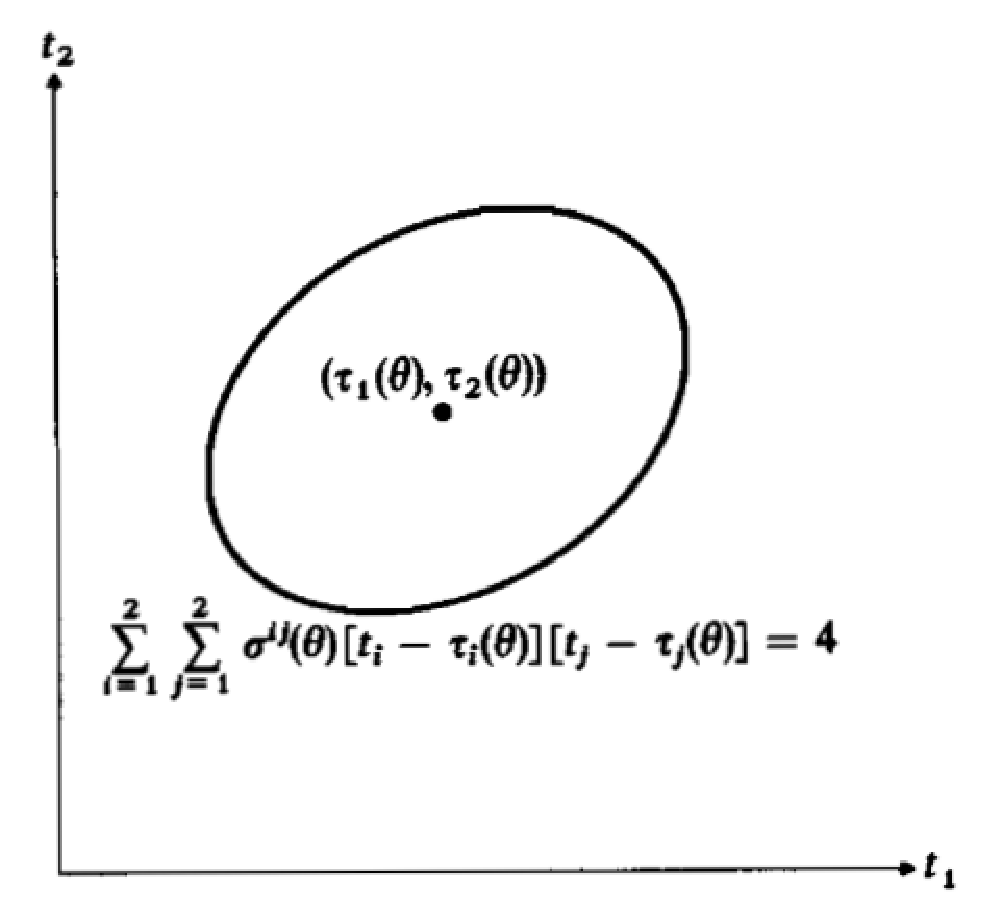
\includegraphics[scale = 0.5]{pictures/ellipsoid_of_concentration.eps}
\caption{Elipsoid koncentrace pro $r = 2$}
\label{ellipsoid-of-concentration}
\end{figure}

Elipsoid koncentrace tedy měří, jak je $(T_1, ..., T_r)$ ``koncentrováno'' okolo $(\tau_1(\theta), ..., \theta_r(\theta))$. Funkce odhadu $(T_1, ..., T_r)$, jejíž elipsoid koncentrace je obsažen v elipsoidu koncentrace jiné funkce odhadu $(T_1', ..., T_r')$, je více ``koncentrován'' okolo $\tau_1(\theta), ..., \tau_r(\theta)$ než $(T_1', ..., T_r')$.

Determinant kovarianční matice funkce odhadu je proporcionální čtverci plochy odpovídajícímu elipsoidu koncentrace. Tímto se dostáváme k Wilksově zobecnění rozptylu.

\begin{definition}[Wilksovo zobecnění rozptylu]
Uvažujme nezkreslenou funkci odhadu $(T_1, ..., T_r)$ pro $(\tau_1(\theta), ..., \tau_r(\theta))$. Wilkosův zobecněný rozptyl funkce odhadu $(T_1, ..., T_r)$ je definován jako determinant její kovarianční matice.
\end{definition}

Následující věta představuje zobecnění věty (7.9) pro $r$ dimenzí. Tuto větu uvádíme bez důkazu.
\begin{theorem}
Uvažujme náhodný výběr $X_1, ..., X_n$ z populace $f(x; \theta_1, ..., \theta_k)$. Nechť $S_1 = \mathfrak{s}_1(X_1, ..., X_n), ..., S_m = \mathfrak{s}_m(X_1, ..., X_n)$ jsou sdruženě dostatečné statistiky a nechť $(T_1, ..., T_r)$ představuje nezkreslenou funkci odhadu pro $(\tau_1(\theta), ..., \tau_r(\theta))$. Definujme $T_j' = E[T_j|S_1, ..., S_m]$ pro $j = 1, ..., r$. Pak
\begin{enumerate}
\item $(T_1', ..., T_r')$ je statistika a nezkreslená funkce odhadu pro $(\tau_1(\theta), ..., \tau_r(\theta))$ a $T_j' = \mathfrak{t}_j'(S_1, ..., S_m)$, tj. $T_j'$ je funkcí sdruženě dostatečných statistik $S_1, ..., S_m$.
\item $D_{\theta}[T_j'] \le D_{\theta}[T_j]$ pro každé $\theta \in \overline{\underline{\Theta}}$.
\item Elipsoid koncentrace pro $(T_1', ..., T_r')$ je obsažen v elipsoidu koncentrace pro $(T_1, ..., T_r)$ pro každé $\theta \in \overline{\underline{\Theta}}$.
\end{enumerate}
\end{theorem}

Bod (2) implikuje
\begin{equation*}
\sum_{j = 1}^r a_j D_{\theta}[T_j'] \le \sum_{j = 1}^r a_j D_{\theta}[T_j] ~~~\textit{pro}~ a_j \le 0
\end{equation*}
a bod (3) implikuje, že Wilksův zobecněný rozptyl pro $(T_1', ..., T_r')$ je menší než Wilksův zobecněný rozptyl pro $(T_1, ..., T_r)$.

Větu (7.11) lze taktéž zobecnit pro $r$ dimenzí. Nejprve je však třeba zobecnit koncept úplnosti.

\begin{definition}[Sdružená kompletnost]
Uvažujme náhodný výběr $X_1, ..., X_n$ z populace $f(x; \theta_1, ..., \theta_k)$. Nechť $(T_1, ..., T_m)$ představuje soubor statistik. Statistiky $T_1, ..., T_m$ nazýváme sdruženě kompletní, jestliže $E_{\theta}[\mathit{z}(T_1, ..., T_m)] \equiv 0$ pro všechna $\theta \in \overline{\underline{\Theta}}$ implikuje $P_{\theta}[\mathit{z}(T_1, ..., T_m) = 0] \equiv 1$ pro všechna $\theta \in \overline{\underline{\Theta}}$, kde $\mathit{z}(T_1, ..., T_m)$ je statistikou.
\end{definition}

\begin{example}
Uvažujme náhodný výběr z poulace $f(x; \theta_1, \theta_2) = \frac{1}{\theta_2 - \theta_1}I_{(\theta_1, \theta_2)}(x)$, kde $\theta_1 < \theta_2$. Definujme $\theta = (\theta_1, \theta_2)$, $Y_1 = \min(X_1, ..., X_n)$ a $Y_n = \max(X_1, ..., X_n)$. Pokusme se dokázat, že $X_1$ a $X_n$ jsou sdruženě kompletní\footnote{Z předchozího textu již víme, že jsou sdruženě dostatečné.}.

Uvažujme nezkreslenou funkci odhadu $\mathit{z}(Y_1, Y_n)$ pro 0, tj.
\begin{equation*}
E_{\theta}[\mathit{z}(Y_1, ..., Y_n)] \equiv 0 ~~~ \textit{pro všechna}~\theta \in \Theta
\end{equation*}
Dále
\begin{gather*}
E_{\theta}[\mathit{z}(Y_1, Y_n)] = \int \int \mathit{z}(y_1, y_n)f_{Y_1, Y_n}(y_1, y_n)d y_1 d y_n\\
= \int_{\theta_1}^{\theta_2}\left(\int_{\theta_1}^{y_n}\mathit{z}(y_1, y_n) n(n - 1)\left(\frac{y_n - \theta_1}{\theta_2 - \theta_1} - \frac{y_1 - \theta_1}{\theta_2 - \theta_1}\right)^{n - 2} \frac{1}{\theta_2 - \theta_1}\frac{1}{\theta_2 - \theta_1}dy_1\right)dy_n
\end{gather*}
což je shodou okolností rovno nule jen tehdy, jestliže
\begin{equation*}
\int_{\theta_1}^{\theta_2} \int_{\theta_1}^{y_n} \mathit{z}(y_1, y_n)(y_n - y_1)^{n - 2}dy_1 dy_n \equiv 0 ~~~ \textit{pro}~\theta_1 < \theta_2
\end{equation*}
Derivací obou stran vzhledem k $\theta_2$ získáme
\begin{equation*}
\int_{\theta_1}^{\theta_2} \mathit{z}(y_1, \theta_2)(\theta_2 - y_1)^{n - 2}dy_1 \equiv 0 ~~~ \textit{pro všechna}~\theta_1 < \theta_2
\end{equation*}
Následnou derivací dle $\theta_1$ získáme
\begin{equation*}
-\mathit{z}(\theta_1, \theta_2)(\theta_2 - \theta_1)^{n-2} \equiv 0 ~~~\textit{pro všechna}~\theta_1 < \theta_2
\end{equation*}
a proto $\mathit{z}(\theta_1, \theta_2) = 0$ pro $\theta_1 < \theta_2$, tj. $\mathit{z}(\theta_1, \theta_2) = 0$ pro $y_1 < y_n$. $Y_1$ a $Y_n$ jsou tak sdruženě kompletní.
\end{example}

Jestliže je $f(x; \theta_1, ..., \theta_k)$ je členem $k$-parametrické rodiny exponenciálních rozdělení, pak lze soubor sdruženě kompletních a dostatečných statistik nalézt s pomocí následující věty. Tato věta, kterou uvádíme bez důkazu, je zobecněním věty (7.10). Navíc jsou opomenuty některé podmínky regularity, a proto není zcela přesně formulována.

\begin{theorem}
Uvažujme náhodný výběr z populace $f(x; \theta_1, ..., \theta_k)$. Jestliže je  $f(x; \theta_1, ..., \theta_k)$ členem $k$-parametrické rodiny exponenciálních rozdělení, tj.
\begin{equation*}
f(x; \theta_1, ..., \theta_k) = a(\theta_1, ..., \theta_k)b(x)e^{\sum_{j = 1}^k c_j(\theta_1, ..., \theta_k)d_j(x)}
\end{equation*}
pak $\left(\sum d_1(X_i), ..., \sum d_k(X_i)\right)$ představuje soubor minimálních sdruženě kompletních a dostatečných statistik.
\end{theorem}

\begin{example}
Uvažujme náhodný výběr $X_1, ..., X_n$ z populace
\begin{equation*}
f(x; \theta_1, \theta_2) = \phi_{\theta_1, \theta_2^2}(x) = \frac{1}{\sqrt{2 \pi}\theta_2}e^{-\frac{1}{2}\left(\frac{x - \theta_1}{\theta_2}\right)^2}
\end{equation*}
Výše uvedenou pravděpodobnostní funkci lze také vyjádřit jako
\begin{equation*}
f(x; \theta_1, \theta_2) = \frac{1}{\sqrt{2 \pi} \theta_2}e^{-\frac{1}{2}\left(\frac{\theta_1}{\theta_2}\right)^2}e^{-\frac{x^2}{2 \theta_2^2} + \frac{\theta_1 x}{\theta_2^2}}
\end{equation*}
a proto jsou, dle výše uvedené věty, $\sum X_i$ a $\sum X_i^2$ sdruženě kompletní a dostatečné statistiky.
\end{example}

Následující věta je vektorovou analogií věty (7.11). Jestliže definujeme UMVUE jako optimum, pak lze s pomocí následující věty identifikovat optimální funkci odhadu pro vektor funkcí parametrů.

\begin{theorem}
Uvažujme náhodný výběr $X_1, ..., X_n$ z populace $f(x; \theta_1, ..., \theta_k)$. Definujme $\theta = (\theta_1, ..., \theta_k)$. Jestliže $S_1 = \mathfrak{s}_1(X_1, ..., X_n), ..., S_m = \mathfrak{s}_m(X_1, ..., X_n)$ jsou sdruženě kompletní a dostatečné statistiky a jestliže existuje nezkreslená funkce odhadu pro $(\tau_1(\theta), ..., \tau_r(\theta))$, pak existuje jedinečná nezkreslená funkce odhadu $T_1^* = \mathfrak{t}_1^*(S_1, ..., S_m), ..., T_r^* = \mathfrak{t}_r^*(S_1, ..., S_m)$ pro $(\tau_1(\theta), ..., \tau_r(\theta))$, která splňuje
\begin{itemize}
\item $D_{\theta}[T_j^*] \le D_{\theta}[T_j]$ pro každé $\theta \in \overline{\underline{\Theta}}$, $j = 1, ..., r$ a libovolnou alternativní funkci odhadu $(T_1, ..., T_r)$ pro $(\tau_1(\theta), ..., \tau_r(\theta))$,
\item Elipsoid koncentrace pro $(T_1^*, ..., T_r^*)$ je obsažen v elipsoidu koncentrace pro $(T_1, ..., T_r)$, kde $(T_1, ..., T_r)$ je libovolná alternativní nezkreslená funkce odhadu pro $(\tau_1(\theta), ..., \tau_r(\theta))$.
\end{itemize}
\end{theorem}

Funkci odhadu $(T_1^*, ..., T_r^*)$ lze nalézt dvěma způsoby. Prvním je kvalifikovaný odhad $\mathfrak{t}_1^*, ..., \mathfrak{t}_r^*$, které představují funkce sdruženě kompletních a dostatečných statistik $S_1, ..., S_m$ a které budou nezkreslenými funkcemi odhadu pro $(\tau_1(\theta), ..., \tau_r(\theta))$. Druhým způsobem je nalezení libovolného souboru nezkreslených funkcí odhadu pro $(\tau_1(\theta), ..., \tau_r(\theta))$ a následný výpočet jejich podmíněné střední hodnoty pro daný soubor sdruženě kompletních a dostatečných statistik $S_1, ..., S_m$.

\begin{example}
Uvažujme náhodný výběr z populace $f(x; \theta_1, \theta_2) = \frac{1}{\theta_2 - \theta_1}I_{(\theta_1, \theta_2)}(x)$. Pokusme se ``sdruženě'' odhadnout $\tau_1(\theta) = \theta_2 - \theta_1$ a $\tau_2(\theta) = \frac{\theta_1 + \theta_2}{2}$.

Z předchozího textu víme, že $Y_1 = \min(X_1, ..., X_n)$ a $Y_n = \max(X_1, ..., X_n)$ jsou sdruženě kompletní a dostatečné statistiky. Abychom tak našli nezkreslenou funkci odhadu $(T_1^*, T_2^*)$ s uniformě nejmenším rozptylem, stačí nalézt nezkreslenou funkci odhadu, která je funkcí těchto statistik. Protože $E[Y_1] = \theta_1 + \frac{\theta_2 - \theta_1}{n + 1}$ a $E[Y_n] = \theta_2 - \frac{\theta_2 - \theta_1}{n + 1}$, představuje $\left(\frac{n + 1}{n - 1}(Y_n - Y_1), \frac{Y_1 + Y_n}{2}\right)$ námi hledanou nezkreslenou funkci odhadu pro $\left(\theta_2 - \theta_1, \frac{\theta_1 + \theta_2}{2}\right)$.
\end{example}

\begin{example}
Uvažujme náhodný výběr $X_1, ..., X_n$ z normálního rozdělení $f(x; \theta_1, \theta_2) = \phi_{\mu, \sigma^2}(x)$. Z předchozího textu víme, že $\sum X_i$ a $\sum X_i^2$ jsou sdruženě kompletní a dostatečné statistiky. Proto na základě věty (7.20) je $\left(\sum \frac{X_i}{n}, \sum \frac{(X_i - \overline{X})^2}{n - 1}\right)$ nezkreslenou funkcí odhadu pro $(\mu, \sigma^2)$ jejíž elipsoid koncentrace je obsažen v elipsoidu koncentrace libovolné alternativní funkce odhadu\footnote{Protože $\sum(X_i - \overline{X})^2 = \sum X_i^2 - n \overline{X}^2$, je funkce odhadu $\frac{\sum (X_i - \overline{X})^2}{n - 1}$ funkcí sdruženě kompletních a dostatečných statistik $\sum X_i$ a $\sum X_i^2$.}.

Nyní předpokládejme, že chceme získat funkci odhadu pro $\theta = (\mu, \sigma^2)$ při splnění podmínky
\begin{equation*}
\int_{\tau(\theta)}^{\infty}\phi_{\mu, \sigma^2}(x)dx = \alpha
\end{equation*}
pro známé a fixní $\alpha$. $\tau(\theta)$ je $(1 - \alpha)$-tý kvantil, tj. splňuje podmínku $P[X_i > \tau(\theta)] = \alpha$. To implikuje $1 - \alpha = \Phi\left(\frac{\tau(\theta) - \mu}{\sigma}\right)$ neboli $\tau(\theta) = \mu + z_{1 - \alpha}\sigma$, kde $z_{1 - \alpha}$ je definováno vztahem $\Phi(z_{1 - \alpha}) = 1 - \alpha$. Abychom našli UMVUE pro $\tau(\theta)$, stačí nalézt nezkreslenou funkci odhadu pro $\mu + z_{1 - \alpha}\sigma$, která je sama funkcí $\sum X_i$ a $\sum X_i^2$. Protože $\overline{X}$ je UMVUE pro $\mu$ a protože lze dokázat, že
\begin{equation*}
\frac{\Gamma\left(\frac{n - 1}{2}\right)}{\Gamma \left(\frac{n}{2}\right) \sqrt{2}}\sqrt{\sum_{i = 1}^n(X_i - \overline{X})^2} = T^*
\end{equation*}
je UMVUE pro $\sigma$, je $\overline{X} + z_{1 - \alpha}T^*$ UMVUE pro $\tau(\theta)$. Při odvození jsme aplikovali větu (7.20) pro $r = 1$.
\end{example}

\section{Odhad maximální věrohodnosti}

Uvažujme náhodný výběr $X_1, ..., X_n$ z populace $f(\cdot, \theta)$, kde $\theta$ je reálné číslo. Pro pozorované hodnoty $x_1, ..., x_n$ je odhad $\hat{\theta}$ parametru $\theta$ dán maximem funkce věrohodnosti
\begin{equation*}
L(\theta; x_1, ..., x_n) = \prod_{i = 1}^n f(x_i, \theta)
\end{equation*}
Označme funkci odhadu založenou na principu maximální věrohodnosti jako $\hat{\Theta}_n = \hat{\zeta}_n(X_1, ..., X_n)$. Z předchozího textu víme, že je žádoucí, aby funkce odhadu splňovala některé podmínky.
\begin{theorem}
Uvažujme náhodný výběr $X_1, ..., X_n$ z populace $f(x, \theta)$, kde $f(x, \theta)$ splňuje určité podmínky regularity. Je-li $\hat{\Theta} = \hat{\zeta}_n(X_1, ..., X_n)$ funkcí odhadu dle maximální věrohodnosti pro $\theta$, pak
\begin{enumerate}
\item $\hat{\Theta}_n$ je asymptoticky normálně rozdělené se střední hodnotou $\theta$ a rozptylem $\frac{1}{n}E\left[\left(\frac{\partial}{\partial \theta} \ln(f(X, \theta))\right)^2\right]$,
\item posloupnost funkcí odhadu $\hat{\Theta}_1, ..., \hat{\Theta}_n$ je BAN.
\end{enumerate}
\end{theorem}

Výše uvedená věta, kterou nebudeme dokazovat, říká, že pro náhodné výběry velkého rozsahu je funkce odhadu pro $\theta$ založená na metodě maximální věrohodnosti nejlepší možnou funkcí odhadu\footnote{Mohou existovat jiné funkce odhadu, které budou stejně dobré ale ne lepší.}. Dále platí, že rozptyl asymptotického normálního rozdělení v bodě (1) je Cramér-Raovou dolní mezí rozptylu.

\begin{example}
Uvažujme náhodný výběr $X_1, ..., X_2$ z negativního exponenciálního rozdělení $f(x, \theta) = \theta e^{-\theta x}I_{[0, \infty)}(x)$. Lze odvodit, že funkce odhadu dle maximální věrohodnosti pro $\theta$ je $\frac{\sum X_i}{n} = \frac{1}{\overline{X}}$. Dle výše uvedené věty má tato funkce odhadu asymptoticky normální rozdělení se střední hodnotou $\theta$ a rozptylem\footnote{Viz. příklad (7.31)}
\begin{equation*}
\frac{1}{n E_{\theta}\left[\left(\frac{\partial}{\partial \theta}\ln(f(X, \theta))\right)\right]} = \frac{\theta^2}{n}
\end{equation*}
\end{example}

Dle věty (7.2) je funkce odhadu pro $\tau(\theta)$ daná metodou maximální věrohodnosti $\tau(\hat{\Theta})$. Jestliže má $\tau(\cdot)$ derivaci prvního stupně, lze dokázat, že $\tau(\hat{\Theta})$ má asymptoticky normální rozdělení se střední hodnotou $\tau(\theta)$ a rozptylem
\begin{equation*}
\frac{[\tau'(\theta)]^2}{n E_{\theta}\left[\left(\frac{\partial}{\partial \theta}\ln(f(X, \theta))\right)^2\right]}
\end{equation*}
který představuje Cramér-Raovu dolní mez rozptylu.

Funkce odhadu dle metody maximální věrohodnosti si zachovává výše uvedené vlastnosti také v případě, kdy je $\theta$ $k$-rozměrným vektorem. Lze totiž opět dokázat, že při splnění určitých podmínek regularity, lze funkce odhadu popsat pomocí asymptotického vícerozměrného normálního rozdělení. Je-li např. $k = 2$, tj. $\theta = (\theta_1, \theta_2)$, sledují $\hat{\Theta}_1$ a $\hat{\Theta}_2$ asymptoticky dvourozměrné normální rozdělení s parametry
\begin{gather*}
\mu_1 = \theta_1\\
\sigma_1^2 = - \frac{E_{\theta}\left[\frac{\partial^2}{\partial \theta_2^2}\ln(f(X, \theta))\right]}{n \Delta}\\
\mu_2 = \theta_2\\
\sigma_2^2 = - \frac{E_{\theta}\left[\frac{\partial^2}{\partial \theta_1^2}\ln(f(X, \theta))\right]}{n \Delta}\\
\rho_{\sigma_1, \sigma_2} = \frac{E_{\theta}\left[\frac{\partial^2}{\partial \theta_2 \theta_1}\ln(f(X, \theta))\right]}{n \Delta}
\end{gather*}
kde
\begin{equation*}
\Delta = E_{\theta}\left[\frac{\partial^2}{\partial \theta_1^2}\ln(f(X, \theta))\right]E_{\theta}\left[\frac{\partial^2}{\partial \theta_2^2}\ln(f(X, \theta))\right] - \left(E_{\theta}\left[\frac{\partial^2}{\partial \theta_1 \theta_2}\ln(f(X, \theta))\right]\right)^2
\end{equation*}

\begin{example}
Uvažujme náhodný výběr z populace
\begin{equation*}
f(x, \theta) = f(x; \theta_1, \theta_2) = \phi_{\theta_1, \theta_2}(x) = \frac{1}{\sqrt{2 \pi \theta_2}}e^{-\frac{1}{2 \theta_2}(x - \theta_1)^2}
\end{equation*}
V předchozích příkladech jsme odvodily funkce odhadu dle metody maximální věrohodnosti pro $\theta_1$ a $\theta_2$.
\begin{gather*}
\hat{\Theta}_1 = \frac{1}{n}\sum_{i = 1}^n X_i\\
\hat{\Theta}_2 = \frac{1}{n}\sum_{i = 1}^n (X_i - \hat{\Theta}_1)^2
\end{gather*}
Asymptotické dvourozměrné normální rozdělení $\hat{\Theta}_1$ a $\hat{\Theta}_2$ má střední hodnoty $\theta_1$ a $\theta_2$. Protože $\ln(f(X, \theta)) = -\frac{1}{2}\ln(\theta_2) - \frac{1}{2 \theta_2}(X - \theta_1)^2$, jsou hledané derivace
\begin{gather*}
\frac{\partial^2}{\partial \theta_1^2} \ln(f(X, \theta)) = -\frac{1}{\theta_2}\\
\frac{\partial^2}{\partial \theta_2 \theta_1} \ln(f(X, \theta)) = -\frac{X - \theta_1}{\theta_2^2}\\
\frac{\partial^2}{\partial \theta_2^2} \ln(f(X, \theta)) = \frac{1}{2 \theta_2^2} -\frac{(X - \theta_1)^2}{\theta_2^3}\\
\end{gather*}
Platí
\begin{gather*}
E[X] = \theta_1\\
E[(X - \theta_1)^2] = \theta_2\\
-E_{\theta}\left[\frac{\partial^2}{\partial \theta_1^2} \ln(f(X, \theta))\right] = \frac{1}{\theta_2}\\
-E_{\theta}\left[\frac{\partial^2}{\partial \theta_2 \partial \theta_1}\ln(f(X, \theta))\right] = 0\\
-E_{\theta}\left[\frac{\partial^2}{\partial \theta_2^2} \ln(f(X, \theta))\right] = \frac{1}{2\theta_2^2}\\
\end{gather*}
což implikuje $\Delta = \frac{1}{2 \theta_2^2}$. Zbývající parametry dvourozměrného normálního rozdělení tak jsou $\sigma_1^2 = \frac{\theta_2}{n}, \sigma_2^2 = \frac{2 \theta_2^2}{n}$ a $\rho = 0$.
\end{example}


